\ifx\allfiles\undefined

% 如果有这一部分另外的package,在这里加上
% 没有的话不需要

\begin{document}
	\else
	\fi
	
%\setchapterpreamble[u]{\margintoc}
\chapter{李群(Lie Group)与李代数(Lie Algebra)}
\labch{intro}


\section*{章节导论:对称性与对称性破缺}
仍在画饼,可以参考这篇知乎文章,写的很不错:\href{https://zhuanlan.zhihu.com/p/338221764}{知乎专栏}




\section{李群(Lie Group)初步}
\subsection{群与李群(Lie Group)}
我们或许听说过一个说法:``物理学的关键是对称和守恒",而诺特定理给出了对称性与守恒性的联系,例如,时间平移不变性意味着能量守恒;空间平移不变性意味着动量守恒;转动不变性意味着角动量守恒;电势和向量势的规范不变性得出电荷的守恒等.而描述对称性的语言就是群论.


我们可以认为群是一类拥有特殊结构的集合,即满足如下关系的集合\sidenote[][]{当然,这里会忽略对于主线无用的那些群论内容,所以如果和数学系的抽象代数对比,你甚至可能会感觉到学的不是同一个东西}:
\marginnote[]{这一章虽然名字比较吓人,但并没有太过深入讲解李群与李代数,主要为了帮助物理系学生来快速对这一门学科建立印象.当然,我们不能保证在后续的不断更新中是否会改变这一点,在最初的版本中,这一章被置于第三章,也就是初量的后续部分,以及这一章的进度只会跟进后续章节的需要,也就是说这一章的全部已完成内容足以支撑起后续章节的学习.}
\begin{definition}[群的定义]
    设$G$是一个集合,若满足下面4个条件,则称$G$为一个群(Group)
    \begin{enumerate}
        \item $G$中存在一种运算规则,对$G$中的任意两个元素$g,h\in G$,存在对应$G$中的一个元素,记为
        \begin{equation}
            k=g\circ h(k=gh)
        \end{equation}
        \item 运算规则满足交换律,对$G$中的任意三个元素$g,h,k\in G$,存在
        \begin{equation}
            (gh)k=g(hk)
        \end{equation}
        \item $G$中存在一个幺元$e$(有时也称单位元),使得对于$G$中任意元素$g$,均有
        \begin{equation}
            ge=eg=g
        \end{equation}
        \item $G$中每一个元素$g$,均存在一逆元$g^{-1}$,使得
        \begin{equation}
            gg^{-1}=g^{-1}g=e
        \end{equation}
    \end{enumerate}
\end{definition}
我们可以发现,群的运算规则通常不满足交换律,特殊的,我们把满足交换律的群称为阿贝尔群(Abel Group)\sidenote[][]{关于这个有一个经典笑话:一位美国数学教授来到法国,见路边有一小孩,遂上前问到:“小朋友,你知道1+2等于几吗?”小孩摇摇头说:“不知道.”教授正想感叹法国数学教育如此之落后,却听到小孩接着说:“虽然我不知道1+2等于几,但是我知道1+2等于2+1,因为整数加法群是阿贝尔群!”}.
\begin{definition}[子群的定义]
    设$G$是一个群,$H$为$G$的一个子集($H\subseteq G$),若$H$按照$G$的运算规则仍是一个群,则称$H$是$G$的子群.
\end{definition}
下面我们将给出一系列典型的群的实例,请根据定义思考它们是怎么构成的,并且尝试找到一些共性.
\begin{example}
    全体实数$\mathbb{R}$(或复数$\mathbb{C}$),对加法构成一个阿贝尔群.\\
    我们知道有理数全体是$\mathbb{R}$的子群,而全体偶数是有理数的子群,自然也是$\mathbb{R}$的子群,那么存在一个问题:无理数全体,或奇数全体是否是$\mathbb{R}$的子群?
    \sidenote[][]{都不是,首先对于无理数我们注意到$\pi+(-\pi)=0$,而0不是无理数,故无理数不构成加法群.同样的,我们注意到$1+(-1)=0$,0同样也不是奇数,故奇数也不构成加法群.}
\end{example}
\begin{example}
    全体实数除去零$\mathbb{R}/0$或全体复数除去零$\mathbb{C}/0$对乘法构成阿贝尔群.\\
    同样的,我们有个问题:为什么要除去0?\sidenote{答案是显然的,群中幺元为1,但$0/0$无意义.}
\end{example}
\begin{example}
    $G =\{1,-1,i,-i\}$对复数乘法运算构成一有限阿贝尔群.这里1是$G$的幺元,而-1的逆元就是-1,$i$与$-i$互为逆元.
\end{example}
\begin{example}
    行列式不为零的n阶实矩阵全体对矩阵乘法构成一个群,$n$阶全线性群,其记为$GL(n,R)$,它的元素由$n^2$个独立实参数所确定.其是一个$n^2$维(不可交换)李群,在后面我们会再次讨论它.
\end{example}
\begin{example}
    行列式为 1 的 2 阶实矩阵全体对矩阵乘法构成一个群:二阶(实)特殊线性群$SL(2,R)$.因为二阶实矩阵$\begin{bmatrix}a&b\\c&d\end{bmatrix}$由四个实数$a,b,c,d$ 构成,由于行列式为1的要求,使他们必须满足条件:$ad-bc=1$.所以$SL(2,R)$ 中的元素由3个独立的实参数所确定.按照下面将要给出的定义可见$SL(2,R)$ 是一个三维(不可交换)李群,而且它是$GL(2,R)$的子群.
\end{example}
\begin{example}
    行列式为 1 的 n 阶实矩阵全体对矩阵乘法构成一个群:n阶特殊线性群$SL(n,R)$,这是一个$n^2-1$维(不可交换)李群,而且它是$GL(n,R)$的子群.
\end{example}
\begin{example}
    行列式不为0的 n 阶复矩阵全体对矩阵乘法构成一个群:n阶(复)全线性群$GL(n,C)$,行列式为 1 的 n 阶复矩阵全体对矩阵乘法构成一个群:n阶(复)特殊线性群$SL(n,C)$.\\
    $GL(n,C)$是一个$2n^2$维(不可交换)李群,$SL(n,C)$是一个$2n^2-12$维(不可交换)李群.
\end{example}

我们发现,所举的例子(除第一个外)都存在共同点:元素都是矩阵(实数和复数可看作一阶矩阵),群的运算法则都是矩阵乘法.我们把这类群统称为\textbf{线性群},线性群也是最具代表性的一类李群,今后所使用的李群基本上都是线性群.
\marginnote[]{事实上,从现在开始,我们就已经走上物理的道路上了,实际上,哪怕你掌握了这一章的全部内容,可能对于数学上的抽象代数那一套仍非常陌生,但早已足够应付物理上的内容了.在上一段,我们给出了一个断言:``今后所使用的李群基本上都是线性群",实际上,我们完全可以这么说,如果不去碰高能和那些fancy的理论(例如弦论,Ads/CFT等),哪怕仅掌握$U(1),SU(2),SU(4)$,$SO(2),SO(3)$这几个群和其表示论对于凝聚态学习就远远足够了.}

下面我们正式进入李群这一部分的内容.
\begin{definition}[Lie群的定义]
    设$G$是一个$r$维流形,同时$G$又是一个群,并将其幺元记为$e$,因$e$又是流形$G$中的一点,所以可取定一个包含$e$的局部坐标邻域$U$;在$U$中取定坐标系$\{U,\varphi\}$.设取$e$为坐标原点,有
    \begin{equation}
        \varphi(e)=(0,0,\cdots,0)
    \end{equation}
    任取$U$中的三个元素$g,h,k$,并设其坐标为
    \begin{equation}
        \begin{aligned}
            \varphi(g)&=(x_1,x_2,\cdots,x_r)\\
            \varphi(h)&=(y_1,y_2,\cdots,y_r)\\
            \varphi(k)&=(z_1,z_2,\cdots,z_r)
        \end{aligned}
    \end{equation}
    而群乘法$k=gh$则可以被定义为以下形式:
    \begin{equation}
        \begin{aligned}
            &z_{1}=f_{1}(x_{1},\cdots,x_{r};y_{1},\cdots,y_{r})\\
            &z_{2}=f_{2}(x_{1},\cdots,x_{r};y_{1},\cdots,y_{r})\\
            &z_{r} =f_r(x_1,\cdots,x_r;y_1,\cdots,y_r) 
        \end{aligned}
    \end{equation}
    我们要求这$r$个函数$f_1,f_2,\cdots,f_r$是无限次可导的(光滑的).我们把这$r$个函数$f_1,f_2,\cdots,f_r$称为$G$的\textbf{乘法函数}.其完全确定了群$G$的结构.我们把这样的群$G$叫做一个$r$维李群.
\end{definition}
我们现在根据群的定义来给出几个自然性质
\begin{enumerate}
    \item 第一个定义是显然的,因为李群的定义建立在这种运算规则上,我们只需要对另外3个条件进行讨论.
    \item 我们现在给出交换律所导出的性质,为方便表述,我们简记群乘法关系为$z=f(x,y)$:
    \begin{equation}
        f(f(x,y),z)=f(x,f(y,z))
    \end{equation}
    \item 对于幺元$e$,其坐标为$(0,0,\cdots,0)$,所以有$ex=xe=x$.
    \begin{equation}
        f(x,0)=f(0,x)=x
    \end{equation}
    \item 对于逆元$g^{-1}$,我们设其坐标为$(\tilde{x}_1,\cdots\tilde{x}_r)$,于是有
    \begin{equation}
        f(x,\tilde{x})=f(\tilde{x},x)=0
    \end{equation}
\end{enumerate}
我们很容易看出,乘法函数是很抽象的,只有乘法函数来研究李群往往是无处下手的(更何况我们是学物理的),于是有了李代数的理论.不过在展开李代数之前,我们使用几个实际的李群的例子来帮助建立对于李群的理解.
\begin{example}
    $T_2=\Big\{\begin{bmatrix}e^{x_1}&x_2\\0&1\end{bmatrix}\Big|x_1,x_2\in\mathbb{R}\Big\}$.这个群的元素由两个独立实参数$x_1,x_2$决定.所以,$T_2$是一个二维流形\sidenote[][]{流形:一句话来表述是将一个空间的局部近似为一个欧氏空间,我们把这个欧氏空间称为流形(manifold),你可以把它当做一种空间.}.我们现在来逐个验证其满足群的要求.
\end{example}
\begin{proof}
    \begin{enumerate}
        \item 首先我们验证其封闭性
        \begin{equation}
            \begin{gathered}\begin{bmatrix}e^{x_1}&x_2\\0&1\end{bmatrix}\begin{bmatrix}e^{y_1}&y_2\\0&1\end{bmatrix}=\begin{bmatrix}e^{x_1}e^{y_1}&e^{x_1}y_2+x_2\\0&1\end{bmatrix}\\=\begin{bmatrix}e^{x_1+y_1}&e^{x_1}y_2+x_2\\0&1\end{bmatrix}=\begin{bmatrix}e^{z_1}&z_2\\0&1\end{bmatrix}\in T_2\end{gathered}
        \end{equation}
        并同时写出其乘法函数,不难发现其乘法函数是无限次可微的.
        \begin{equation}
            \begin{aligned}&z_{1}=f_{1}(x_{1},x_{2};y_{1},y_{2})=x_{1}+y_{1},\\&z_{2}=f_{2}(x_{1},x_{2};y_{1},y_{2})=e^{x_{1}}y_{2}+x_{2}.\end{aligned}
        \end{equation}
        \item $T_2$的乘法运算为矩阵乘法,自然满足结合律.
        \item 对于幺元,我们注意到
        \begin{equation}
            \begin{bmatrix}e^0&0\\0&1\end{bmatrix}=\begin{bmatrix}1&0\\0&1\end{bmatrix}
        \end{equation}
        \item 我们注意到有
        \begin{equation}
            \begin{aligned}\begin{bmatrix}e^{-x_1}&-x_2e^{-x_1}\\0&1\end{bmatrix}\begin{bmatrix}e^{x_1}&x_2\\0&1\end{bmatrix}&=\begin{bmatrix}e^{x_1}&x_2\\0&1\end{bmatrix}\begin{bmatrix}e^{-x_1}&-x_2e^{-x_1}\\0&1\end{bmatrix}\\&=\begin{bmatrix}1&0\\0&1\end{bmatrix}\end{aligned}
        \end{equation}
        所以逆元为$\begin{bmatrix}e^{-x_1}&-x_2e^{-x_1}\\0&1\end{bmatrix}$并容易验证其不满足交换律.
    \end{enumerate}
\end{proof}
\begin{example}
    我们的下一个实例是绕定轴转动的旋转群SO(2),显然,我们只需要一个变量(转动角$\theta$)就可以表述一个转动变换,所以我们表示群元为$g(\theta)$,其中$\theta$的取值范围是$[0,2\pi)$.而群的运算法则可以被规定为相继的两个转动,即转动角相加,但需要保持转动角始终在取值范围内.我们可以使用公式表达:
    \begin{equation}
        g(\theta_1)g(\theta_2)=g(\theta_{12}),\qquad\theta_{12}=(\theta_1+\theta_2)\mod 2\pi
    \end{equation}
    我们容易验证其满足对应的4条性质.不过我们在关于线性代数的学习中,我们知道:我们也可以使用旋转矩阵来表述定轴转动.
    \begin{equation}
        \begin{bmatrix}x\\y\end{bmatrix}\xrightarrow{g(\theta)}\begin{bmatrix}x'\\y'\end{bmatrix}=\begin{bmatrix}\cos\theta&-\sin\theta\\\sin\theta&\cos\theta\end{bmatrix}\begin{bmatrix}x\\y\end{bmatrix}=\begin{bmatrix}x\cos\theta-y\sin\theta\\x\sin\theta+y\cos\theta\end{bmatrix}
    \end{equation}
    我们发现,旋转矩阵是SO(2)群的群元.我们在下一个例子会更加深入讨论这部分内容.
\end{example}
\begin{example}
    现在我们需要讨论三维旋转群SO(3),其群元表示三维空间中绕某个固定点的一个转动$g\in SO(3)$,为了方便表述SO(3),我们使用如图所示的欧拉(Euler)角$(\alpha,\beta,\gamma)$来表示一个转动.
    \begin{marginfigure}
        \centering
        \includegraphics[width=0.4\linewidth]{"images/Euler angle"}
        \caption{欧拉角}
        \label{fig:euler-angle}
    \end{marginfigure}
    \marginnote[*6]{我们依次写出绕$z$轴旋转$\alpha$角;绕$x$轴旋转$\beta$角;绕$z$轴旋转$\gamma$角的三个群元的矩阵表示:
    $$g_z^\alpha={\begin{bmatrix}\cos \alpha &-\sin \alpha &0\\\sin \alpha &\cos \alpha &0\\0&0&1\end{bmatrix}}$$
    $$g_x^\beta={\begin{bmatrix}1&0&0\\0&\cos \beta &-\sin \beta \\0&\sin \beta &\cos \beta \end{bmatrix}}$$
    $$g_z^\gamma={\begin{bmatrix}\cos \gamma &-\sin \gamma &0\\\sin \gamma &\cos \gamma &0\\0&0&1\end{bmatrix}}$$
    }

    我们给出最终群元的表示:
    \begin{equation}
        g=g_z^\alpha g_x^\beta g_z^\gamma
    \end{equation}
    因此,SO(3)的元素可以通过三个独立参量$\alpha,\beta,\gamma$来确定,因此不难验证SO(3)是一个三维李群.
    
    现在我们给出另一种表述SO(3)的方法.\\
    我们对于两个矢量$x=(x_1,x_2,x_3),y=(y_1,y_2,y_3)$给出三维欧式空间$\mathbb{R}_3$的内积:
    \begin{equation}
        \langle x,y\rangle=\sum_{j=1}^{3}x_j y_j=x_1y_1+x_2y_2+x_3y_3
    \end{equation}
    我们定义一个线性变换算符$g=(g_{ij})$,存在关系
    \begin{equation}
        \begin{aligned}
            x\xrightarrow{g}x'=gx=\begin{bmatrix}g_{11}&g_{12}&g_{13}\\g_{21}&g_{22}&g_{23}\\g_{31}&g_{32}&g_{33}\end{bmatrix}\begin{bmatrix}x_1\\x_2\\x_3\end{bmatrix}\\ g\in SO(3)\Leftrightarrow\langle gs,gy\rangle=\langle x,y\rangle\quad\forall x,y\in\mathbb{R}_3\quad\text{且}\det g>0
        \end{aligned}
    \end{equation}
    而且我们发现$\langle gs,gy\rangle=\langle x,g^Tgy\rangle$,其中$g^T$表示$g$的转置,即$g_{ij}^T=g_{ij}$,我们根据刚才所给出的关系发现$\langle x,g^Tgy\rangle=\langle x,y\rangle$,即$g^Tg=\textbf{1}$,我们把满足关系$g^Tg=gg^T$的线性变换构成的群称为正交群.
    
    对于3阶矩阵$g$,存在9个元素,但为了满足特殊正交群的特殊性($\det g=1$)和正交性($g^Tg=gg^T$),共有6个方程需要满足.所以,我们可以拿出3个作为独立参数,这再次证明了$g$可以表述SO(3)这个三维李群.
\end{example}
\subsection{指数映射与对数映射}
\marginnote[]{在前面的部分,我们强调了群的乘法一般不可交换,这直接导致了刻画李群的乘法函数变得非常复杂,这意味着想通过研究乘法函数来研究李群是不现实的.而为了研究李群的各种结构,我们可以对李群在幺元处的无穷小变换进行研究,而Lie证明了李群的主要特征可以通过无穷小变换来得到,这就是为什么现在称这类群为李群的原因.}对于无穷小变换,它是一个拥有特殊结构的线性空间,我们称它构成的代数结构为\textbf{李代数}.

这里,我们再次强调,后面默认所有的群都是\textbf{线性群},群的运算规则都是\textbf{矩阵乘法}!

我们回到这一节前面所提到的,由于矩阵乘法不可交换,导致运算变得复杂,那么有没有一种办法,可以让复杂的运算变为较简单的运算呢(最好还是物理中最喜欢的线性运算)?

答案是肯定的,我们高中就学过一种特殊的运算:指数运算,它可以把较为复杂的乘法变为较为简单的加法,即对于给出的$y_1=e^{x_1},y_2=e^{x_2}$,我们有
\begin{equation}
    y_1y_2=e^{x_1}e^{x_2}=e^{x_1+x_2}
\end{equation}
这样,我们就实现了运算的``降级",并且还是线性运算.现在,问题变为,我们能否同样应用这种方式,将矩阵乘法转变为某种加法呢?

答案同样是肯定的,但由于矩阵乘法比代数乘法更为复杂,相应的``加法"自然也更加复杂.而为了得到这种简单的``加法"运算,我们首先对$n$阶矩阵$A$定义幂指数:
\begin{equation}
    e^A=\exp(x)=\textbf{1}+A+\frac{A^2}{2!}+\frac{A^3}{3!}+\cdots 
\end{equation}
易证此级数对于任意的矩阵$A$都是收敛的.并且对于零矩阵$O$,显然有
\begin{equation}
    e^O=\textbf{1}
\end{equation}
并且,前面我们多次提到矩阵乘法相比代数乘法是不可交换的,那么,反应到对应的``加法"运算上,自然也有区分加法的性质,即当且仅当$A,B$对易的时候,才有$e^Ae^B=e^{A+B}$,这是主要的困难点,那么我们的主要问题就集中在$e^Ae^B=e^{?}$上,这也就是我们将要学习的李代数的内容.不过,在正式开始李代数的内容之前,我们先讨论一下其他同样有价值的内容.

我们仅了解了和指数函数对应的运算,而我们高中还知道,指数函数的逆运算是对数函数,接下来我们效仿之前的内容,对对数函数应用同样的定义方法:

同样对于$n$阶矩阵$A$,我们定义\sidenote[][]{在物理的语境中,$\log$通常仅指$\ln$,同样的,本文中采取该写法.}
\begin{equation}
    \log A=(A-\textbf{1})-\frac{(A-\textbf{1})^2}2+\frac{(A-\textbf{1})^3}3-\frac{(A-\textbf{1})^4}4+\cdots 
\end{equation}
不同于指数函数,为了保证级数收敛,我们要求$A-\textbf{1}$的每一个元素的绝对值均小于$\dfrac{1}{n}$,即要求$A$是与幺元邻近的元素.并且指数函数与对数函数互为逆运算的关系对于这个定义同样适用(仅需泰勒展开即可证明,留给读者自行尝试).
\subsection{单参数子群}
在前面,我们通过代数方法初步建立了一些对应关系,这一小节,我们通过几何的角度再次考虑这个对应关系.

\begin{definition}[单参数子群]
    设$G$为一个李群,并且$\gamma(t)(-\infty<t<\infty)$为$g$中过幺元$e$的一条曲线,则对每一取定的$t_0\in \mathbb{R},\gamma(t_0)$是$G$中的一个元素.并设参数$t$满足:
    \begin{equation}
        \gamma(t_1+t_2)=\gamma(t_1)\gamma(t_2)
    \end{equation}
    则称$\gamma(t)$是$G$中的一个单参数李群.
\end{definition}

现在我们通过几何的角度思考问题.

我们将李群$G$的一个单参数子群看成流形$G$ (对二维Lie 群,可将$G$ 看成为一张曲面)中过$e$处的一条曲线.从微积分知道这只要对$\gamma\left(t\right)$在$t=0$处求导即得$\gamma\left(t\right)$在$t=0$处的切向量,$\gamma^\prime(0)=\frac{\d\gamma(t)}{\d t}$.(因为我们只讨论线性群,所以$\gamma\left(t\right)$是矩阵,其元素是$t$ 的函数,$\gamma^{\prime}(t)$ 表示对$\gamma(t)$的每一元素求导所得的矩阵).由于:
\begin{equation}
    \gamma (t+s)=\gamma (t)\gamma (s)
\end{equation}
两边对$s$求导,同时令$s=0$,得到一个微分方程
\begin{equation}
    \gamma' (t)=\gamma(t)\gamma' (0)
\end{equation}
对于这类微分方程,我们知道其解为
\begin{equation}
    \gamma(t)=\exp(t\gamma'(0))
\end{equation}
由此,我们知道,单参数子群必能表达为指数映射的形式.\\
\begin{marginfigure}
    \centering
    \caption{二维李群与其单参数子群}
    
    
    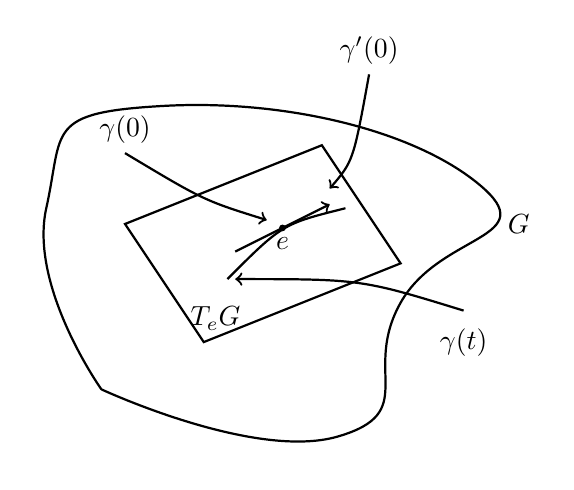
\begin{tikzpicture}
        
        % Draw the manifold G
        \draw[thick] plot [smooth,tension=1] 
        coordinates {(0.2,1.4) (3.2,0.8) (4,2.5) (5,4) (1,5) (-0.5,3.7) (0.2,1.4)};
        %\draw[thick] (0,0) to[out=30, in=180] (4,2.5) to[out=0, in=270] (5,4) to[out=90, in=30] (1,5) to[out=210, in=150] cycle;
        
        % Label G
        \node at (5.5,3.5) {$G$};
        
        % Draw the tangent space T_eG
        \draw[thick] (1.5, 2) -- (4, 3) -- (3, 4.5) -- (0.5, 3.5) -- cycle;
        
        % Label TeG
        \node at (1.65, 2.3) {$T_e G$};
        
        % Draw the curve \gamma(t)
        \draw[thick] (1.8, 2.8) .. controls (2.5, 3.5) .. (3.3, 3.7);
        
        % Label points and vectors
        \node at (0.5,4.7) {$\gamma(0)$};
        \draw[thick, ->] (0.5,4.4) .. controls (1.5,3.8) .. (2.3,3.55);
        \node at (4.8, 2) {$\gamma(t)$};
        \draw[thick, ->] (4.8,2.4) .. controls (3.5,2.8) .. (1.9,2.8);
        \filldraw[black] (2.5,3.45) circle (1pt) node[anchor=north] {$e$};
        \draw[thick, ->] (1.9, 3.15) -- (3.1, 3.75);
        \node at (3.6, 5.7) {$\gamma'(0)$};
        \draw[thick, ->] (3.6, 5.4) .. controls (3.4,4.3) .. (3.1,3.95);
        
    \end{tikzpicture}
\end{marginfigure}
由解的形式可见,对于$G$在幺元处的切空间$T_eG$的任意一个向量$A=\gamma'(0)$,就有$G$中的一元素$\gamma(1)=\exp(\gamma'(0))$与之对应.现在我们稍微总结一下:对于李群$G$这个流形,我们可以找到其单参数子群$T_eG$作为其切空间,并且我们可以找到一个指数映射从切空间到原空间,很快,当我们学会李代数的时候,我们会再次使用李代数的语言来总结:``李代数就是李群的切空间所导出的代数".

我们再次回到群$G$和它的单参数子群,我们发现,如果给定$G$中与幺元邻近的一个元素\sidenote[][]{当然,由于我们研究线性群,幺元为单位矩阵.}$g$,并定义向量$A=\log g$,则由$e^A=g$ 知,$A$ 为$G$ 在$e$ 处之切向量,$e^tA$为以 $A$ 为单位切向量的单参数子群.因此,对$G$ 中与幺元$e$ 邻近的一个元素就有$T_{e}(G)$($G$ 在幺元处的切空间)中一向量$A$ 与之对应,也就是说,设$U\subset G$ 中包含$e$ 的一个适当邻域,我们建立了一种对应关系
\begin{equation}
    \begin{aligned}
        G\supset U&\overunderset{\log}{\exp}{\longleftrightarrow}T_{e}(G)\\g&\to A=\log g\\e^{A}&\leftarrow A
    \end{aligned}
\end{equation}
这种对应关系可以使我们对李群的研究转化到与其对应的在幺元$e$处的切空间$T_e(G)$.而我们知道,$T_e(G)$是由向量组成的线性空间,其线性结构具有先天优势,拥有远比李群简单的结构和运算.但由于我们前面所提到的,由于矩阵乘法相比于数乘的不可交互性,自然由此导出的切空间的运算自然也不能简单用普通加减法来表述,即右侧关系图
\marginnote[]{$$\begin{aligned}&T_{e}(G)\qquad G\\&A\quad\longrightarrow\quad e^{A}\\&B\quad\longrightarrow\quad e^{B}\\&A+B\to e^{A+B}\ne e^{A}e^{B}\end{aligned}$$}

为此,我们迫切需要引入一种新的代数结构来反映$G$中的不可交换性,而具有这种新结构的线性空间$T_e(G)$
,就是我们下一节所要讲的\textbf{李代数}.
\section{李群与李代数}
\subsection{李代数}
由上面的讨论,我们现在知道$e^Ae^B\ne e^{A+B}$,那么,问题自然变为:$e^Ae^B=e^{?}$,或者表述为,$G$的单参数子群的代数结构是什么样的?

为了解决这个问题,我们设$A,B\in T_e(G)$,取一个参数$t$,并要求$|t|$适当小,从而能够保证$e^{tA}$与$e^{tB}$均为李群$G$中与幺元$e$邻近的元素\sidenote[][]{这个要求是必要的,我们需要满足后续使用级数的收敛性.}.现在我们构造一个函数:
\begin{equation}
    g(t)=e^{tA}e^{tB}e^{-tA}e^{-tB}
\end{equation}
显然,对于特例,即如果$e^{tA}$与$e^{tB}$可交换,$g(t)=e=\textbf{1}$,对于不可交换的情况,$g(t)$与幺元$e$的偏离程度反映了$e^{tA}$与$e^{tB}$的乘法与可交换的乘法之间的差异大小.现在我们具体分析$g(t)$.
\marginnote[*-2]{展开的计算过程
$$\begin{aligned}
    g(t)& =e^{tA}e^{tB}e^{-tA}e^{-tB} \\
    &=(\textbf{1}+tA+\frac{t^{2}}{2!}A^{2}+\frac{t^{3}}{3!}A^{3}+\cdots)(\textbf{1}+tB+\frac{t^{2}}{2!}B^{2}+\frac{t^{3}}{3!}B^{3}+\cdots) \\
    &(\textbf{1}-tA+\frac{t^2}{2!}A^2-\frac{t^3}{3!}A^3+\cdots)(\textbf{1}-tB+\frac{t^2}{2!}B^2-\frac{t^3}{3!}B^3+\cdots) \\
    &=\{\textbf{1}+t(A+B)+t^{2}(\frac{A^{2}}{2}+AB+\frac{B^{2}}{2})\\&+t^{3}(\frac{A^{3}}{6}+\frac{A^{2}B}{2}+\frac{AB^{2}}{2}+\frac{B^{3}}{6})+O(t^{4})\} \\
    &\{\textbf{1}-t(A+B)+t^2(\frac{A^2}{2}+AB+\frac{B^2}{2})\\&-t^3(\frac{A^3}{6}+\frac{A^2B}{2}+\frac{AB^2}{2}+\frac{B^3}{6})+O(t^4)\} \\
    &=\textbf{1}+t(A+B-A-B)+t^{2}(AB-BA)+t^{3}(\frac{A^{2}B}{2}-\frac{AB^{2}}{2} \\
    &-\frac{B^2A}{2}+\frac{BA^2}{2}-ABA+BAB)+O(t^4) \\
    &=\textbf{1}+t^{2}[A,B]+\frac{t^{3}}{2}([A,[A,B]]-[B,[B,A]])+O(t^{4})
\end{aligned}$$
}
\begin{equation}
    \begin{aligned}
        g(t)& =e^{tA}e^{tB}e^{-tA}e^{-tB} \\
        &=\textbf{1}+t^{2}[A,B]+\frac{t^{3}}{2}([A,[A,B]]-[B,[B,A]])+O(t^{4})
    \end{aligned}
\end{equation}
这里我们使用了对易子记号$[,]$,不过对于李代数,它也称为李括号,李乘法\sidenote[][*5]{事实上,对于线性群它等同于对易子,后面会加以区分的使用对易子和李括号.}.对于函数$g(t)$,我们有
\begin{equation}
    \frac{g(t)-\textbf{1}}{t^2}=[A,B]+O(t)
\end{equation}
因此,考虑极限$t\to0$时,
\begin{equation}
    \lim_{t\to0}\frac{g(t)-\textbf{1}}{t^{2}}=[A,B]
\end{equation}
由此,我们发现李群$G$的元素$e^{tA}$与$e^{tB}$的乘法的不可交换程度在$|t|$很小时主要取决于$[A,B]$

现在我们做变量代换$t=\sqrt{s}$,则
\begin{equation}
    \frac{g(\sqrt{s})-g(0)}{s}=[A,B]+O(\sqrt{s})
\end{equation}
并因此
\begin{equation}
    \lim_{s\to0}\frac{g(\sqrt{s})-g(0)}{s}=[A,B]
\end{equation}
这也说明$[A,B]$是李群$G$中过幺元的曲线$g(\sqrt{s})$在幺元处的\textbf{切向量},即$[A,B]\in T_e(G)$,这也意味着我们证明了如下关系
\begin{equation}
    \forall A,B\in T_{e}(G) , [A,B]\in T_{e}(G)
\end{equation}
即对易子(李括号)对向量空间$T_e(G)$的封闭性.


此时,我们可以回答开头所提到的问题了,不妨设$e^{tA}e^{tB}=e^{tC}$,则
\marginnote[]{展开的计算过程
$$\begin{aligned}
    tC&=\log e^{tC}=\log e^{tA}e^{tB}\\
    &=\log\{(\textbf{1}+t(A+B)+\frac{t^{2}}{2}(A^{2}+2AB+B^{2})+ \\
    &\quad+\frac{t^{3}}{6}(A^{3}+3A^{2}B+3AB^{2}+B^{3})+O(t^{4})\} \\
    &=t(A+B)+\frac{t^{2}}{2}(A^{2}+2AB+B^{2})+\frac{t^{3}}{6}(A^{3}+3A^{2}B+3AB^{2}+B^{3}) \\
    &\quad+O(t^{4})-\{t(A+B)+\frac{t^2}{2}(A^2+2AB+B^2)+O(t^3)\}^2/2+ \\
    &\quad+\{t(A+B)+\frac{t^{2}}{2}(A^{2}+2AB+B^{2})+O(t^{3})\}^{3}/3+O(t^{4}) \\
    &=t(A+B)+\frac{t^{2}}{2}(AB-BA)+\frac{t^{3}}{12}(A^{2}B-ABA-ABA+BA^{2} \\
    &\quad-B^2A+BAB+BAB-AB^2)+O(t^4) \\
    &=(tA+tB)+\frac{1}{2}[tA,tB]+\frac{1}{12}[tA,[tA,tB]-tB,[tB,tA]]+O(t^{4}) 
\end{aligned}$$}
\begin{equation}
\begin{aligned}
    tC&=\log e^{tC}=\log e^{tA}e^{tB}\\
    &=(tA+tB)+\frac{1}{2}[tA,tB]+\frac{1}{12}[tA,[tA,tB]-tB,[tB,tA]]+O(t^{4}) 
\end{aligned}
\end{equation}
由此可见,只要给出李括号,$T_e(G)$中知道了与$e^{tA},e^{tB}$相对应的元素$tA,tB$即可求得$T_e(G)$中与$e^{tA}e^{tB}$相对应的元素.因此,我们认为李括号可以表述李群切空间的代数结构,并对于李括号有如右侧所示的性质.
\marginnote[]{李括号的性质$$\begin{gathered}
        \left\lbrack {A, A}\right\rbrack = 0\\
        \left\lbrack {A, B}\right\rbrack = - \left\lbrack {B, A}\right\rbrack\\
        \left\lbrack {A, c}\right\rbrack = 0\;\left( {c\text{ 只是一个数 }}\right)\\
        \left\lbrack {A + B, C}\right\rbrack = \left\lbrack {A, C}\right\rbrack + \left\lbrack {B, C}\right\rbrack\\
        \left\lbrack {A,{BC}}\right\rbrack = \left\lbrack {A, B}\right\rbrack C + B\left\lbrack {A, C}\right\rbrack\\
        \left\lbrack {A,\left\lbrack {B, C}\right\rbrack }\right\rbrack + \left\lbrack {B,\left\lbrack {C, A}\right\rbrack }\right\rbrack + \left\lbrack {C,\left\lbrack {A, B}\right\rbrack }\right\rbrack = 0
    \end{gathered}$$}

我们称有了李括号的向量空间$T_e(G)$构成一个李代数,更准确的来讲是李群$G$的李代数,并记为$\mathfrak{g}$.\\
李群的李代数完全刻画了李群在幺元附近的结构,而要研究李群在幺元附近的性质只需要研究李代数即可,但是需要注意的是,李代数\textbf{仅}刻画了李群在幺元附近的\textbf{局部}性质,\textbf{不能}反映其整体性质,一个李群对应一个李代数,而一个李代数可以对应多个李群.
\begin{definition}[结构常数]
    设$G$是一个$r$维李群,取定幺元$e$的一个邻域$U$,在$U$中取定坐标系$\{U,\varphi\}$并取$e$为坐标原点:
    \begin{equation}
        \varphi(e)=(0,0,\cdots,0)
    \end{equation}
    对于其的单参数子群,我们有
    \begin{equation}
        \begin{cases}\gamma_j(t),&j=1,2,\cdots,r\\\varphi(\gamma_j(t))=(\underbrace{0,\cdots,0}_{(j-1)\text{个零}},t,0,\cdots,0)\end{cases}
    \end{equation}
    为其$r$条坐标曲线.
    
    以$X_{j}= \gamma _{j}^{\prime }(0),j= 1, 2, \cdots , r$记为其在幺元处的切向量.即$X_j\in T_e(G) = \mathfrak{g}, j= 1, 2, \cdots , r$.显然,$\{X_1,X_2,\cdots,X_r\}$可取作为向量空间$T_{_e}(G)$的基——$T_{e}(G)$中任一向量可用它们的线性组合表出.由于$[X_i,X_j]\in \mathfrak{g}$,所以
    \begin{equation}
        [X_{i},X_{j}]=\sum_{j,k=1}^{n}C_{ij}^{k}X_{k}\quad i,j=1,2,\cdots,r
    \end{equation}
    这$r^3$个数$\{C_{ij}^k\}k,i,j=1,2,\cdots,r$称为李群以$\{X_1,X_2,\cdots,X_r\}$,为基的\underline{结构常数}.
\end{definition}
对于李代数$\mathfrak{g}$中任意向量$X,Y$,有
\begin{equation}
    \begin{aligned}
        X&=\sum_{j=1}^{r}\xi^{j}X_{j}&Y=\sum_{j=1}^{r}\eta^{j}X_{j}\\
        X&\sim(\xi^{1},\xi^{2},\cdots,\xi^{r})&Y=(\eta^{1},\eta^{2},\cdots\eta^{r})\\
        Z&=[X,Y]=\left[\sum_{j=1}^{r}\xi^{j}X_{j},\sum_{k=1}^{r}\eta^{k}X_{k}\right]&=\sum_{i=1}^{r}\sum_{j,k=1}^{r}C_{jk}^{i_{k}}\xi^{j}\eta^{k}X_{i}
    \end{aligned}
\end{equation}
将$Z$也用坐标表示
\begin{equation}
    Z=\sum_{i=1}^{r}\zeta^{ i}X_{i},\quad Z\sim(\zeta^{ 1},\zeta^{ 2},\cdots\zeta^{ r})
\end{equation}
此时易求出结构常数
\begin{equation}
    \zeta^{i}=\sum_{j,k=1}^{r}C_{jk}^{i}\xi^{j}\eta^{k},\quad i=1,2,\cdots,r
\end{equation}
由此可见,结构常数可以完全确定一个李代数.

需要强调的是,结构常数与基的选取有关,而李代数的一个重要的问题就是如何选取适当的基使结构常数最简单.\\
或许到此,你可能还对结构常数一头雾水,在再次讲解结构常数之前,我们还是先给出一些基本性质,并实际算一下结构常数.
\begin{equation}
    \begin{aligned}
        &C_{ij}^{ k}=-C_{ji}^{ k}&i,j,k=1,2,\cdots,r\\
        &\sum_{l=1}^{r}\left(C_{ij}^{l}C_{lk}^{m}+C_{jk}^{l}C_{li}^{m}+C_{ki}^{l}C_{lj}^{m}\right)=0&i,j,k,m=1,2,\cdots,r.\end{aligned}
\end{equation}
\begin{example}
    我们再次考虑由例题3.8给出的群$T_2=\Big\{\begin{bmatrix}e^{x_1}&x_2\\0&1\end{bmatrix}\Big|x_1,x_2\in\mathbb{R}\Big\}$,我们知道$\gamma_1(t)=\begin{bmatrix}e^t&0\\0&1\end{bmatrix} -\infty<t<\infty $与$\gamma_2(t)=\begin{bmatrix}1&t\\0&1\end{bmatrix} -\infty<t<\infty $是$T_2$的两个单参数子群,同时也是过幺元的两条曲线,我们给出在幺元处的切向量$X_1=\gamma_1'(0)=\begin{bmatrix}1&0\\0&0\end{bmatrix},X_2=\gamma_2'(0)=\begin{bmatrix}0&1\\0&0\end{bmatrix}$,因此李群$T_2$的李代数$\mathfrak{t}_2$的基由$X_1,X_2$组成,现在来求结构常数.
    \begin{equation}
        \begin{aligned}&[X_1,X_1]=\begin{bmatrix}0&0\\0&0\end{bmatrix}\quad[X_2,X_2]=\begin{bmatrix}0&0\\0&0\end{bmatrix}\\&[X_1,X_2]=\begin{bmatrix}1&0\\0&0\end{bmatrix}\begin{bmatrix}0&1\\0&0\end{bmatrix}-\begin{bmatrix}0&1\\0&0\end{bmatrix}\begin{bmatrix}1&0\\0&0\end{bmatrix}=\begin{bmatrix}0&1\\0&0\end{bmatrix}=X_2.\end{aligned}
    \end{equation}
    所以,$C_{11}^1=C_{11}^2=C_{22}^1=C_{22}^2=0,\quad C_{12}^1=-C_{21}^1=0,\quad C_{12}^2=1,\quad C_{21}^2=-1.$
\end{example}
\begin{example}
    我们再次回到$SO(3)$群,现在我们来求其李代数$\mathfrak{so}(3)$及其结构常数.\\
    我们列出其群元(绕$x,y,z$的转动),即旋转矩阵,如右侧所示
        \marginnote[*-3]{三个群元的矩阵表示:
        $$g_{x}(t)=\begin{bmatrix}1&0&0\\0&\cos t&-\sin t\\0&\sin t&\cos t\end{bmatrix}$$
        $$g_y(t)=\begin{bmatrix}\cos t&0&\sin t\\0&1&0\\-\sin t&0&\cos t\end{bmatrix}$$
        $$g_{z}(t)=\begin{bmatrix}\cos t&-\sin t&0\\\sin t&\cos t&0\\0&0&1\end{bmatrix}$$
    }

    此时,我们发现,这是其的三个单参数子群,而它们在幺元处的切向量一并给出
    \begin{equation}
        I_{1}=g_{x}'(0),\quad I_{2}=g_{y}'(0),\quad I_{3}=g_{z}'(0).
    \end{equation}
    于是$\{I_1,I_2,I_3\}$构成$SO(3)$的李代数$\mathfrak{so}(3)$的一组基,其李括号为:
    \begin{equation}
        [I_1,I_2]=I_1I_2-I_2I_1=I_3,[I_2,I_3]=I_1,[I_3,I_1]=I_2
    \end{equation}
    同时得出结构常数$C_{12}^{ 1}=0,C_{12}^{ 2}=0,C_{12}^{ 3}=1,\cdots.$
    
    我们可以发现,对于这个李括号,其还等价于三维欧式空间的向量乘法,我们就得到了简单情况下的李括号的退化情况.
\end{example}

%\begin{example}
%	我们这次要讨论的是在物理上极为重要的一类李群:$SU(2)$
%\end{example}
\subsection{李氏三定理和无穷小变换}
1
\subsection{李群的无穷小生成元}
1
\subsection{典型李群和李代数}
1
\section{李代数进阶}
\subsection{张量,不可约张量}
1
\subsection{卡西米尔算符(Casimir operator)}
1
\subsection{典型李代数的二阶卡西米尔算符}
1



%\ifx\allfiles\undefined

% 如果有这一部分另外的package,在这里加上
% 没有的话不需要

\begin{document}
	\else
	\fi
\chapter{量子动力学}
\begin{introduction}
	\item 时间演化算符
	\item 薛定谔方程
	\item 两种绘景
	\item 波动方程
\end{introduction}
到此为止, 我们还没有讨论物理系统如何随时间改变. 本章专门阐述态右矢和/或可观测量的动力学演化. 换言之, 在这一章我们所关心的是牛顿, 或拉格朗日 (Lagrange) 和哈密顿运动方程的量子力学类似方程.

\section{时间演化和薛定谔方程}
我们应当记住的首要之点是: 时间在量子力学中只是一个参量而不是一个算符. 特别地, 时间不是前一章所说的可观测量. 像谈论位置算符一样谈论时间算符是无意义的. 具有讽刺意味的是, 在波动力学发展的历史过程中, 德布罗意也好, 薛定谔也罢都受到过能量与时间为一方及动量与位置 (空间坐标) 为另一方的二者之间协变类比的启发. 然而, 我们现在来看量子力学的最终形式时, 已见不到在时间与空间之间对称处理的踪迹. 场的相对论量子理论确实平等地处理了时间与空间坐标, 但它只是在做出了牺牲, 把位置从可观测量的地位降低到只是一个参量的情况下做到这一点的.

当然,简单来说,时间与空间并不对偶或平权,我们对于时间更多是客观的演化,而不是主观的操纵.
\subsection{时间演化算符}
在这一节我们关注的基本点是: 一个态右矢如何随时间改变? 假定我们有一个物理系统,它的态右矢在 ${t}_{0}$ 时刻由 $|\alpha \rangle$ 表示. 在稍后的时刻,一般而言,该系统不会保持在同样的状态 $|\alpha \rangle$ . 让我们把某稍后时刻与该状态相对应的右矢表示为
\begin{equation}
	\left| {\alpha ,{t}_{0};t}\right\rangle ,\;\left( {t > {t}_{0}}\right)
\end{equation}
其中标出 $\alpha ,{t}_{0}$ 是为了强调该系统在某个较早的参考时刻 ${t}_{0}$ 曾经处于态 $|\alpha \rangle$ . 由于时间被认为是一个连续参量, 我们预期存在
\begin{equation}
	\mathop{\lim }\limits_{{t \rightarrow {t}_{0}}}\left| {\alpha ,{t}_{0};t}\right\rangle = |\alpha \rangle
\end{equation}
但是, 我们也可以用一种简化符号(正如同之前常做的那样)
\begin{equation}
	\left| {\alpha ,{t}_{0};{t}_{0}}\right\rangle = \left| {\alpha ,{t}_{0}}\right\rangle
\end{equation}
来代替它. 我们现在这一节的基本任务是研究一个态右矢的时间演化过程:
\begin{equation}
	\left| {\alpha ,{t}_{0}}\right\rangle = |\alpha \rangle \xrightarrow[]{\text{ 时间演化 }}\left| {\alpha ,{t}_{0};t}\right\rangle
\end{equation}
或者说,我们感兴趣的是,探寻在时间平移变换 ${t}_{0} \rightarrow t$ 下,态右矢如何变化.

就像平移的情况一样,这两个右矢由一个被称之为时间演化算符的 $\mathcal{U}\left( {t,{t}_{0}}\right)$ 联系起来:
\begin{equation}\label{2.5}
	\left| {\alpha ,{t}_{0};t}\right\rangle = \mathcal{U}\left( {t,{t}_{0}}\right) \left| {\alpha ,{t}_{0}}\right\rangle
\end{equation}
我们希望描述时间演化算符的哪些性质呢? 第一个重要的性质源于概率守恒对 $\mathcal{U}\left( {t,{t}_{0}}\right)$ 的幺正性的要求. 假定在 ${t}_{0}$ 时刻态右矢用某个可观测量 $A$ 的本征右矢展开:
\begin{equation}
	\left| {\alpha ,{t}_{0}}\right\rangle = \mathop{\sum }\limits_{{a}^{\prime }}{c}_{{a}^{\prime }}\left( {t}_{0}\right) \left| {a}^{\prime }\right\rangle
\end{equation}
同样地, 在稍后某个时刻, 我们有
\begin{equation}
	\left| {\alpha ,{t}_{0};t}\right\rangle = \mathop{\sum }\limits_{{a}^{\prime }}{c}_{{a}^{\prime }}\left( t\right) \left| {a}^{\prime }\right\rangle
\end{equation}
一般来说, 我们无法指望各个展开系数的模保持相同\footnote{然而,稍后我们将证明,如果哈密顿量与 $A$ 对易,则 $\left| {{c}_{{a}^{\prime }}\left( t\right) }\right|$ 的确等于 $\left| {{c}_{{a}^{\prime }}\left( {t}_{0}\right) }\right|$ .}:
\begin{equation}
	\left| {{c}_{{a}^{\prime }}\left( t\right) }\right| \neq \left| {{c}_{{a}^{\prime }}\left( {t}_{0}\right) }\right|
\end{equation}
例如,考虑一个自旋 $\frac{1}{2}$ 系统,其自旋磁矩受到一个沿 $z$ 方向的均匀磁场的作用. 为确定起见,假定 ${t}_{0}$ 时刻该自旋沿正 $x$ 方向,即发现该系统处在 ${S}_{x}$ 的一个本征态上,其本征值为 $\hbar /2$ . 正如稍后将在本节中定量证明的,随着时间的推移,该自旋在 ${xy}$ 平面上进动. 这意味着,在 $t > {t}_{0}$ 时刻观测到 ${S}_{x}$ +的概率不再是 1,还有有限的概率观测到 ${S}_{x}$ -. 而在所有的时刻,观测到 ${S}_{x} +$ 和 ${S}_{x}-$的概率之和都保持为 1 . 尽管对于各个展开系数有上式, 现在我们采用本征右矢展开的符号, 一般我们一定有
\begin{equation}
	\mathop{\sum }\limits_{{a}^{\prime }}{\left| {c}_{{a}^{\prime }}\left( {t}_{0}\right) \right| }^{2} = \mathop{\sum }\limits_{{a}^{\prime }}{\left| {c}_{{a}^{\prime }}\left( t\right) \right| }^{2}
\end{equation}
另一种表述方式是, 如果态右矢初始时归一到了 1 , 则在所有以后的时刻它一定保持归一到 1 :
\begin{equation}
	\left\langle {\alpha ,{t}_{0} | \alpha ,{t}_{0}}\right\rangle = 1 \Rightarrow \left\langle {\alpha ,{t}_{0};t | \alpha ,{t}_{0};t}\right\rangle = 1
\end{equation}
就像在平移的情况一样, 如果时间演化算符取为幺正算符, 我们就能确保这一性质成立. 为此, 我们将幺正性,
\begin{equation}
	\mathcal{U}^{\dagger}\left( {t,{t}_{0}}\right)\mathcal{U}\left( {t,{t}_{0}}\right) = 1
\end{equation}
取为 $\mathcal{U}$ 算符基本性质中的一个. 这个性质使得许多作者把幺正性视为概率守恒的同义词.

我们要求 $\mathcal{U}$ 算符具有的另外一个特征是它的结合性:
\begin{equation}\label{2.12}
	\mathcal{U}\left( {{t}_{2},{t}_{0}}\right) = \mathcal{U}\left( {{t}_{2},{t}_{1}}\right) \mathcal{U}\left( {{t}_{1},{t}_{0}}\right) ,\;\left( {{t}_{2} > {t}_{1} > {t}_{0}}\right)
\end{equation}
这个方程是说,如果对获得从 ${t}_{0}$ 到 ${t}_{2}$ 的时间演化感兴趣,我们则可以通过考虑先从 ${t}_{0}$ 到 ${t}_{1}$ ,再从 ${t}_{1}$ 到 ${t}_{2}$ 的时间演化得到相同的结果(当然,如果你已经对群论有所了解,很容易发现其构成了一个群). 

类比在平移算符时我们的做法,现在考虑一个无穷小时间演化算符 $\mathcal{U}\left( {{t}_{0} + {\d t},{t}_{0}}\right)$:
\begin{equation}
	\left| {\alpha ,{t}_{0};{t}_{0} + {\d t}}\right\rangle = \mathcal{U}\left( {{t}_{0} + {\d t},{t}_{0}}\right) \left| {\alpha ,{t}_{0}}\right\rangle
\end{equation}
由于连续性,当 ${\d t}$ 趋于零时,该无穷小时间演化算符一定约化为单位算符,
\begin{equation}
	\mathop{\lim }\limits_{{{\d t} \rightarrow 0}}\mathcal{U}\left( {{t}_{0} + {\d t},{t}_{0}}\right) = \textbf{1}
\end{equation}
而且,就像在平移情况中那样,我们预期 $\mathcal{U}\left( {{t}_{0} + {\d t},{t}_{0}}\right)$ 与 \textbf{1} 之差为 ${\d t}$ 的量级.

我们断言, 下式满足所有这些要求
\begin{equation}
	\mathcal{U}\left( {{t}_{0} + {\d t},{t}_{0}}\right) = 1 - {i\Omega \d t}
\end{equation}
其中 $\Omega$ 是一个厄米算符,则显然有
\begin{equation}
	{\Omega }^{ \dagger } = \Omega
\end{equation}
该无穷小时间平移算符同样满足结合性
\begin{equation}
	\mathcal{U}\left( {{t}_{0} + \\d{t}_{1} + \\d{t}_{2},{t}_{0}}\right) = \mathcal{U}\left( {{t}_{0} + \\d{t}_{1} + \\d{t}_{2},{t}_{0} + \\d{t}_{1}}\right) \mathcal{U}\left( {{t}_{0} + \\d{t}_{1},{t}_{0}}\right) 
\end{equation}
它与单位算符只相差一个 ${\d t}$ 量级的项. 幺正性还可以在 ${\left( \\d t\right) }^{2}$ 或更高阶的项可以忽略的
\begin{equation}
	{\mathcal{U}}^{ \dagger }\left( {{t}_{0} + {\d t},{t}_{0}}\right) \mathcal{U}\left( {{t}_{0} + {\d t},{t}_{0}}\right) = \left( {\textbf{1} + i{\Omega }^{ \dagger }{\d t}}\right) \left( {\textbf{1} - {i\Omega \d t}}\right) \simeq \textbf{1}
\end{equation}
算符 $\Omega$ 具有频率或者反比于时间的量纲. 那么存在我们熟悉的具有频率量纲的可观测量吗? 回忆一下,在旧量子论中,假定角频率 $\omega$ 通过普朗克关系
\begin{equation}
	E = \hbar \omega
\end{equation}
与能量联系起来. 现在让我们借用经典力学中哈密顿量是时间演化生成元的概念. 那时自然可以把 $\Omega$ 与哈密顿量算符 $H$ 联系起来:
\begin{equation}
	\Omega = \frac{H}{\hbar }
\end{equation}
综上所述, 无穷小时间演化算符可写为:
\begin{equation}
	\mathcal{U}\left( {{t}_{0} + {\d t},{t}_{0}}\right) = \textbf{1} - \frac{iH\d t}{\hbar }
\end{equation}
其中假定了哈密顿量算符 $H$ 是厄米的. 读者可能要问,这里引入的 $\hbar$ 是否与出现在平移算符表达式中的 $\hbar$ 相同.我们可通过稍后导出的量子力学运动方程与经典运动方程做比较回答这个问题. 结果表明,除非这两个 $\hbar$ 是一样的,否则就不能够得到作为相应量子力学关系式的经典极限关系式
\begin{equation}
	\frac{\d\mathbf{x}}{\d t} = \frac{\mathbf{p}}{m}
\end{equation}
\subsection{薛定谔方程}

我们现在能够推导时间演化算符 $\mathcal{U}\left( {t,{t}_{0}}\right)$ 满足的基本微分方程. 在\ref{2.12}中令 ${t}_{1} \rightarrow t,{t}_{2} \rightarrow t + {\d t}$ ,利用时间演化算符的结合性:
\begin{equation}
	\mathcal{U}\left( {t + {\d t},{t}_{0}}\right) = \mathcal{U}\left( {t + {\d t}, t}\right) \mathcal{U}\left( {t,{t}_{0}}\right) = \left( {\textbf{1} - \frac{iH\d t}{\hbar }}\right) \mathcal{U}\left( {t,{t}_{0}}\right)
\end{equation}
其中的时间差 $t - {t}_{0}$ 不必为无穷小. 我们有
\begin{equation}
	\mathcal{U}\left( {t + {\d t},{t}_{0}}\right) - \mathcal{U}\left( {t,{t}_{0}}\right) = - i\left( \frac{H}{\hbar }\right) {\d t}\mathcal{U}\left( {t,{t}_{0}}\right)
\end{equation}
它可以写成微分方程形式:
\begin{equation}\label{2.25}
	i\hbar \frac{\partial }{\partial t}\mathcal{U}\left( {t,{t}_{0}}\right) = {H\mathcal{U}}\left( {t,{t}_{0}}\right)
\end{equation}
这就是时间演化算符的薛定谔方程. 随时间推移发生的每件事都一定遵从这个基本方程.

方程\ref{2.25}立刻导致了一个态右矢满足的薛定谔方程. 用 $\left| {\alpha ,{t}_{0}}\right\rangle$ 右乘\ref{2.25}的两边得到
\begin{equation}
	i\hbar \frac{\partial }{\partial t}\mathcal{U}\left( {t,{t}_{0}}\right) \left| {\alpha ,{t}_{0}}\right\rangle = {H\mathcal{U}}\left( {t,{t}_{0}}\right) \left| {\alpha ,{t}_{0}}\right\rangle
\end{equation}
但是 $\left| {\alpha ,{t}_{0}}\right\rangle$ 不依赖于 $t$ ,所以该式与
\begin{equation}\label{2.27}
	i\hbar \frac{\partial }{\partial t}\left| {\alpha ,{t}_{0};t}\right\rangle = H\left| {\alpha ,{t}_{0};t}\right\rangle
\end{equation}
是相同的, 其中用到了\ref{2.25}.

如果 $\mathcal{U}\left( {t,{t}_{0}}\right)$ 已经给出,并进一步知道了 $\mathcal{U}\left( {t,{t}_{0}}\right)$ 如何作用于初始态右矢 $\left| {\alpha ,{t}_{0}}\right\rangle$ ,就没有必要为求解态右矢的薛定谔方程操心. 我们所须做的就是把 $\mathcal{U}\left( {t,{t}_{0}}\right)$ 作用在 $\left| {\alpha ,{t}_{0}}\right\rangle$ 上,用这种方法我们可以求得任意时刻 $t$ 的态右矢. 因此,我们的第一个任务就是推导出时间演化算符的薛定谔方程的形式解. 存在三种需要分别处理的情况:

情况 1. 哈密顿量算符不依赖时间. 这时我们指的是,甚至当参量 $t$ 改变时,哈密顿量算符也保持不变. 比如,一个自旋磁矩与一个时间无关的磁场相互作用的哈密顿量就是这种情况. 在这种情况下的解由下式给出:
\begin{equation}
	\mathcal{U}\left( {t,{t}_{0}}\right) = \exp \left\lbrack \frac{-{iH}\left( {t - {t}_{0}}\right) }{\hbar }\right\rbrack
\end{equation}
为了证明这一点, 让我们将该指数展开如下(幂级数展开):
\begin{equation}
	\exp \left\lbrack \frac{-{iH}\left( {t - {t}_{0}}\right) }{\hbar }\right\rbrack = 1 + \frac{-{iH}\left( {t - {t}_{0}}\right) }{\hbar } + \left\lbrack \frac{{\left( -i\right) }^{2}}{2}\right\rbrack {\left\lbrack \frac{H\left( {t - {t}_{0}}\right) }{\hbar }\right\rbrack }^{2} + \cdots
\end{equation}
由于这个展开式对时间微商为
\begin{equation}
	\frac{\partial }{\partial t}\exp \left\lbrack \frac{-{iH}\left( {t - {t}_{0}}\right) }{\hbar }\right\rbrack = \frac{-{iH}}{\hbar } + \left\lbrack \frac{{\left( -i\right) }^{2}}{2}\right\rbrack 2{\left( \frac{H}{\hbar }\right) }^{2}\left( {t - {t}_{0}}\right) + \cdots
\end{equation}
我们所得出的解显然满足微分方程\ref{2.25}. 因为 $t \rightarrow {t}_{0}$ 时,求出的解约化为单位算符, 边界条件也被同时满足.求解的另一种方法是相继地组合无穷小时间演化算符:
\begin{equation}
	\mathop{\lim }\limits_{{N \rightarrow \infty }}{\left\lbrack \textbf{1} - \frac{\left( {{iH}/\hbar }\right) \left( {t - {t}_{0}}\right) }{N}\right\rbrack }^{N} = \exp \left\lbrack \frac{-{iH}\left( {t - {t}_{0}}\right) }{\hbar }\right\rbrack
\end{equation}

情况 2. 哈密顿量算符与时间相关,但不同时间的 $H$ 对易. 作为一个例子,让我们考虑一个自旋磁矩受到一个强度随时间改变但方向保持不变的磁场的作用. 此时\ref{2.25}式的形式解为
\begin{equation}
	\mathcal{U}\left( {t,{t}_{0}}\right) = \exp \left\lbrack {-\left( \frac{i}{\hbar }\right) \int_{{t}_{0}}^{t}\d{t}^{\prime }H\left( {t}^{\prime }\right) }\right\rbrack
\end{equation}
它可以用类似的方法证明. 我们只要把情况一中的 $H\left( {t - {t}_{0}}\right)$ 换成 $\int_{{t}_{0}}^{t}\d{t}^{\prime }H\left( {t}^{\prime }\right)$ 即可.

情况 3. 不同时刻的 $H$ 不对易. 继续用与自旋磁矩相关的例子,这一次我们假定磁场的方向也随着时间改变: $t = {t}_{1}$ 时沿 $x$ 方向, $t = {t}_{2}$ 时沿 $y$ 方向等. 因为 ${S}_{x}$ 与 ${S}_{y}$ 不对易, 所以 $H\left( {t}_{1}\right)$ 和 $H\left( {t}_{2}\right)$ 的行为像 $\mathbf{S} \cdot \mathbf{B}$ ,也不对易. 在这种情况下,形式解由下式给出:
\begin{equation}
	\mathcal{U}\left( {t,{t}_{0}}\right) = 1 + \mathop{\sum }\limits_{{n = 1}}^{\infty }{\left( \frac{-i}{\hbar }\right) }^{n}\int_{{t}_{0}}^{t}\d{t}_{1}\int_{{t}_{0}}^{{t}_{1}}\d{t}_{2}\cdots \int_{{t}_{0}}^{{t}_{n - 1}}\d{t}_{n}H\left( {t}_{1}\right) H\left( {t}_{2}\right) \cdots H\left( {t}_{n}\right)
\end{equation}
该式有时称为戴森 (Dyson) 级数, 它以 F. J. 戴森的名字命名, 因为他在量子场论中发展了这种形式的微扰展开. 我们现在不证明这个式子, 因为其证明非常类似于在后续所提到的相互作用绘景中时间演化算符的证明.

在初等应用中,只有情况 1 是实际感兴趣的. 在本章余下的部分,我们假定 $H$ 算符是时间无关的.

\subsection{能量本征右矢}
为了能够计算时间演化算符作用于一个一般初始右矢 $|\alpha \rangle$ 的效应,我们必须首先知道它如何作用于展开 $|\alpha \rangle$ 时使用的基右矢. 如果所用的基右矢是满足
\begin{equation}
	\left\lbrack {A, H}\right\rbrack = 0
\end{equation}
的 $A$ 的本征右矢,那就简单了. 那时, $A$ 的本征右矢也是 $H$ 的本征右矢,称之为\textbf{能量本征右矢},它的本征值用 ${E}_{{a}^{\prime }}$ 表示:
\begin{equation}
	H\left| {a}^{\prime }\right\rangle = {E}_{{a}^{\prime }}\left| {a}^{\prime }\right\rangle
\end{equation}
我们现在可以用 $\left| {a}^{\prime }\right\rangle \left\langle {a}^{\prime }\right|$ 展开时间演化算符. 为简单起见,取 ${t}_{0} = 0$ ,我们得到
\begin{equation}
	\begin{aligned}
		\exp ( \frac{-{iHt}}{\hbar }) &= \mathop{\sum }\limits_{{a}^{\prime }}\mathop{\sum }\limits_{{a}^{\prime \prime }}| {a}^{\prime \prime }\rangle \langle {{a}^{\prime \prime }| {\exp ( \frac{-{iHt}}{\hbar }) }| {a}^{\prime }}\rangle \langle {a}^{\prime }|\\
		&=\mathop{\sum }\limits_{{a}^{\prime }}\left| {a}^{\prime }\right\rangle \exp \left( \frac{-i{E}_{{a}^{\prime }}t}{\hbar }\right) \left\langle {a}^{\prime }\right|
	\end{aligned}
\end{equation}
一旦初始右矢利用 $\left\{ \left| {\alpha }^{\prime }\right\rangle \right\}$ 的展开知道了,则写成这种形式的时间演化算符就使我们能够求解任何初值问题. 作为例子, 假定初始右矢的展开为
\begin{equation}
	\left| {\alpha ,{t}_{0} = 0}\right\rangle = \mathop{\sum }\limits_{{a}^{\prime }}\left| {a}^{\prime }\right\rangle \left\langle {{a}^{\prime } | \alpha }\right\rangle = \mathop{\sum }\limits_{{a}^{\prime }}{c}_{{a}^{\prime }}\left| {a}^{\prime }\right\rangle
\end{equation}
则我们就有
\begin{equation}
	\left| {\alpha ,{t}_{0} = 0;t}\right\rangle = \exp \left( \frac{-{iHt}}{\hbar }\right) \left| {\alpha ,{t}_{0} = 0}\right\rangle = \mathop{\sum }\limits_{{\alpha }^{\prime }}\left| {\alpha }^{\prime }\right\rangle \left\langle {{\alpha }^{\prime } | \alpha }\right\rangle \exp \left( \frac{-i{E}_{{\alpha }^{\prime }}t}{\hbar }\right)
\end{equation}
换句话说, 展开系数随时间变化如下
\begin{equation}
	{c}_{{a}^{\prime }}\left( {t = 0}\right) \rightarrow {c}_{{a}^{\prime }}\left( t\right) = {c}_{{a}^{\prime }}\left( {t = 0}\right) \exp \left( \frac{-i{E}_{{a}^{\prime }}t}{\hbar }\right)
\end{equation}
其模保持不变. 注意, 各分量之间的相对位相的确是随时间改变, 因为振荡的频率各不相同.

一种有意思的特殊情况是,初态碰巧是 $\left\{ \left| {a}^{\prime }\right\rangle \right\}$ 自身中的一个. 初始时,我们有
\begin{equation}
	\left| {\alpha ,{t}_{0} = 0}\right\rangle = \left| {a}^{\prime }\right\rangle
\end{equation}
而在一个稍后的时刻
\begin{equation}
	\left| {a,{t}_{0} = 0;t}\right\rangle = \left| {a}^{\prime }\right\rangle \exp \left( \frac{-i{E}_{{a}^{\prime }}t}{\hbar }\right)
\end{equation}

因此,如果初始时系统是 $A$ 和 $H$ 的一个共同本征态,它在所有的时刻都将保持如此. 最多可能发生的是相位的调制,即 $\exp \left( {-i{E}_{{a}^{\prime }}t/\hbar }\right)$ . 在这个意义上说,一个与 $H$ 相容的可观测量是一个\textit{运动常数}. 当讨论海森堡运动方程时, 我们将再次遇到这种联系的不同形式.

在前面的讨论中,\textit{量子力学的基本任务被简化为寻找一个与 $H$ 对易的可观测量并计算它的本征值.} 一旦完成了这一步, 我们就可以用那个可观测量的本征右矢展开初始右矢, 然后只要用时间演化算符去作用即可. 最后的这一步只不过意味着改变每个展开系数的相位.

尽管我们解决了只有一个与 $H$ 对易的可观测量 $A$ 的情况,当存在几个相互相容且均与 $H$ 对易的可观测量时:
\begin{equation}
	\left\lbrack {A, B}\right\rbrack = \left\lbrack {B, C}\right\rbrack = \left\lbrack {A, C}\right\rbrack = \cdots = 0
\end{equation}
\begin{equation}
	\left\lbrack {A, H}\right\rbrack = \left\lbrack {B, H}\right\rbrack = \left\lbrack {C, H}\right\rbrack = \cdots = 0
\end{equation}
我们的考虑能够很容易地被推广.我们有
\begin{equation}
	\exp \left( \frac{-{iHt}}{\hbar }\right) = \mathop{\sum }\limits_{{K}^{\prime }}\left| {K}^{\prime }\right\rangle \exp \left( \frac{-i{E}_{{K}^{\prime }}t}{\hbar }\right) \left\langle {K}^{\prime }\right|
\end{equation}
其中只要 ${a}^{\prime },{b}^{\prime },{c}^{\prime },\cdots$ 被确定了, ${E}_{{K}^{\prime }}$ 也就唯一地被确定了. 因此,找到一个\textit{相互相容而且还与 $H$ 对易的可观测量的完备集}是关键. 只要找到这样的一个集合,我们就可以把这个初始右矢表示为 $A, B, C,\cdots$ 与 $H$ 的共同本征右矢的叠加. 最后一步只是使用了写成上面形式的时间演化算符. 用这样一种方法,我们可以求解具有时间无关 $H$ 的最普遍的初值问题.
\subsection{期望的时间依赖}
接下来我们要开始研究一个可观测量的期望作为关于时间函数如何变化. 假定 $t = 0$ 时初态是一个与 $H$ 对易的可观测量 $A$ 的一个本征态. 我们现在看一下某个不必与 $A$ 或 $H$ 对易的可观测量 $B$ 的期望. 因为在稍后的时刻这个态右矢为
\begin{equation}
	\left| {{a}^{\prime },{t}_{0} = 0;t}\right\rangle = \mathcal{U}\left( {t,0}\right) \left| {a}^{\prime }\right\rangle
\end{equation}
故 $\langle B\rangle$ 由下式给出
\begin{equation}
	\begin{aligned}
		\langle B\rangle &= \left( {\left\langle {{a}^{\prime } | {\mathcal{U}}^{\dagger}\left( {t,0}\right) }\right\rangle \cdot B \cdot \left\langle {\mathcal{U}\left( {t,0}\right) | {a}^{\prime }}\right\rangle }\right)\\
		&= \left\langle {{a}^{\prime }\left| {\;\exp \left( \frac{i{E}_{{a}^{\prime }}t}{\hbar }\right) B\exp \left( \frac{-i{E}_{{a}^{\prime }}t}{\hbar }\right) }\right. {a}^{\prime }}\right\rangle\\
		&= \left\langle {{a}^{\prime }\left| B\right| {a}^{\prime }}\right\rangle
	\end{aligned}
\end{equation}
它是\textit{不依赖于 $t$} 的. 所以一个可观测量对于能量本征态的期望不随时间变化. 由于这个原因, 能量的本征态经常被称为\textbf{定态}.

对能量本征态的一个\textit{叠加}或一个\textbf{非定态}取期望的时候, 情况更为有趣. 假定初始时有
\begin{equation}
	\left| {\alpha ,{t}_{0} = 0}\right\rangle = \mathop{\sum }\limits_{{a}^{\prime }}{c}_{{a}^{\prime }}\left| {a}^{\prime }\right\rangle
\end{equation}
很容易算出 $B$ 的期望为
\begin{equation}
	\begin{aligned}
		\langle B\rangle &= \left\lbrack {\mathop{\sum }\limits_{{a}^{\prime }}{c}_{{a}^{\prime }}\left\langle {{a}^{\prime }\left| {\exp \left( \frac{i{E}_{{a}^{\prime }}t}{\hbar }\right) }\right| \cdot B \cdot \left\lbrack {\mathop{\sum }\limits_{{a}^{\prime }}{c}_{{a}^{\prime }}\exp \left( \frac{-i{E}_{{a}^{\prime }}t}{\hbar }\right) }\right\rbrack {a}^{\prime \prime }}\right\rangle }\right\rbrack\\
		&= \mathop{\sum }\limits_{{a}^{\prime }}\mathop{\sum }\limits_{{a}^{\prime \prime }}{c}_{{a}^{\prime }}^{ * }{c}_{{a}^{\prime \prime }}\left\langle {{a}^{\prime }\left| B\right| {a}^{\prime \prime }}\right\rangle \exp \left\lbrack \frac{-i\left( {{E}_{{a}^{\prime \prime }} - {E}_{{a}^{\prime }}}\right) t}{\hbar }\right\rbrack
	\end{aligned}
\end{equation}
于是, 这时期望是由一些振荡项组成, 它们的角频率由波尔频率条件
\begin{equation}
	{\omega }_{{a}^{\prime }{a}^{\prime }} = \frac{\left( {E}_{{a}^{\prime }} - {E}_{{a}^{\prime }}\right) }{h}
\end{equation}
确定.
\subsection{自旋进动}
在这里最恰当的是给出一个例子. 我们考虑一个极为简单、然而却能阐明我们所发展的基本形式框架的系统.

我们从一个自旋为 $\frac{1}{2}$ 的系统的哈密顿量
\begin{equation}
	H = - \left( \frac{e}{{m}_{e}c}\right) \mathbf{S} \cdot \mathbf{B}
\end{equation}
(对于电子 $e < 0$ ) 出发,该系统具有 $e\hbar /2{m}_{e}c$ 的磁矩,受到一个外磁场 $\mathbf{B}$ 作用. 此外,我们取 $\mathbf{B}$ 为一个沿 $z$ 方向的均匀静磁场. 这时我们可把 $H$ 记为
\begin{equation}
	H = - \left( \frac{eB}{{m}_{r}c}\right) {S}_{z}
\end{equation}
因为 ${S}_{z}$ 与 $H$ 只差一个常数因子,所以它们显然对易. ${S}_{z}$ 的本征态也是能量本征态,其相应的本征值为
\begin{equation}
	{E}_{ \pm } = \mp \frac{e\hbar B}{2{m}_{e}c},\;\text{ 对于 }{S}_{z} \pm
\end{equation}
最方便的做法是以下述方式定义一个 $\omega$
\begin{equation}
	\omega \equiv \frac{\left| e\right| B}{{m}_{e}c}
\end{equation}
它使两个能量本征值之差为 $\hbar \omega$ . 然后我们就可以把算符 $H$ 简单地改写为
\begin{equation}
	H = \omega {S}_{z}
\end{equation}
此时所有随时间演化的信息全都包含在时间演化算符中
\begin{equation}
	\mathcal{U}\left( {t,0}\right) = \exp \left( \frac{-{i\omega }{S}_{z}t}{\hbar }\right)
\end{equation}
我们将其作用于初态. 展开初始右矢所必须使用的基右矢显然是 ${S}_{z}$ 的本征右矢 $| + \rangle$ 和 $| - \rangle$ ,它们也是能量本征右矢. 假定 $t = 0$ 时刻该系统由下式描写
\begin{equation}
	\left| {\alpha \rangle = {c}_{ + }}\right| + \rangle + {c}_{ - }| - \rangle
\end{equation}
将时间演化算符作用在上面, 我们看到, 态右矢在稍后某时刻为
\begin{equation}
	\left| {\alpha ,{t}_{0} = 0;t}\right\rangle = {c}_{ + }\exp \left( \frac{-{i\omega t}}{2}\right) | {+\rangle + {c}_{ - }\exp \left( \frac{+{i\omega t}}{2}\right) }| - \rangle
\end{equation}
其中我们用到了
\begin{equation}
	H| {\pm \rangle = \left( \frac{\pm \hbar \omega }{2}\right) }| \pm \rangle
\end{equation}
具体地说,让我们假定该初始右矢 $|\alpha \rangle$ 表示自旋向上 (或更精确地说, ${S}_{z} +$ ) 的态$|+\rangle$),它意味着
\begin{equation}
	{c}_{ + } = 1,\;{c}_{ - } = 0
\end{equation}
这告诉我们, 在一个稍后的时刻, 它仍处于自旋向上的态, 这并不奇怪, 因为该态是一个定态.

接下来,让我们假定初始时该系统处在 ${S}_{x} +$ 态. 我们知道
\begin{equation}
	{c}_{ + } = {c}_{ - } = \frac{1}{\sqrt{2}}
\end{equation}
可直截了当地求出在稍后某个时刻 $t$ 系统处于 ${S}_{x} \pm$ 态的概率:
\begin{equation}
	\begin{aligned}
		|\langle S_{s}\pm|\alpha,t_{0}=0;t\rangle|^{2}& = \left|\left[\left(\frac{1}{\sqrt{2}}\right)\langle+|\pm\left(\frac{1}{\sqrt{2}}\right)\langle-|\right.\right]\cdot\left[\left(\frac{1}{\sqrt{2}}\right)\mathrm{exp}\left(\frac{- i \omega t}{2}\right)|+\right] +\left(\frac1{\sqrt{2}}\right)\mathrm{exp}\biggl(\frac{+i\omega t}2\biggr)|-\rangle\biggr]\biggr|^2 \\
		&= \left| \frac{1}{2}\mathrm{exp} \left(\frac{- i \omega t}{2}\right)\pm\frac{1}{2}\mathrm{exp} \left(\frac{+ i \omega t}{2}\right) \right|^{2} \\
		&=\cos^{2}\frac{\omega t}{2}\quad\text{对于}\quad S_{x}+\\
		&=\sin^{2}\frac{\omega t}{2}\quad\text{对于}\quad S_{x}-
	\end{aligned}
\end{equation}
尽管初始时自旋沿正 $x$ 方向,但沿 $z$ 方向的磁场导致它旋转,结果我们得到了在稍后某时刻找到 ${S}_{t}$ 一的有限的概率. 可以看到,这两个概率之和在所有的时刻都是 1,它与时间演化算符的幺正性相符.

我们可以把 ${S}_{x}$ 的期望写成
\begin{equation}
	\begin{aligned}
		\left\langle {S}_{x}\right\rangle &= \left( \frac{\hbar }{2}\right) {\cos }^{2}\left( \frac{\omega t}{2}\right) + \left( \frac{-\hbar }{2}\right) {\sin }^{2}\left( \frac{\omega t}{2}\right)\\
		&= \left( \frac{\hbar }{2}\right) \cos {\omega t}
	\end{aligned}
\end{equation}
故此量随时间振荡,其角频率为相应的两个能量本征值之差除以 $\hbar$ ,它与我们的普遍公式 是一致的. 对 ${S}_{y}$ 和 ${S}_{z}$ 做类似的操作表明
\begin{equation}
	\left\langle {S}_{y}\right\rangle = \left( \frac{\hbar }{2}\right) \sin {\omega t}
\end{equation}
和
\begin{equation}
	\left\langle {S}_{z}\right\rangle = 0
\end{equation}
物理上这意味着自旋在 ${xy}$ 平面上进动. 在后续中讨论转动算符时,我们将进一步评述自旋进动.

自旋进动已被实验严格确证. 事实上, 它被用作研究其他基本量子力学现象的工具. 
\subsection{关联振幅和能量时间不确定度关系}
我们以探讨不同时刻的态右矢如何彼此关联来结束这一节. 假定一个物理系统在 $t = 0$ 时刻的初态右矢由 $|\alpha \rangle$ 定. 它随时间变成 $\left| {\alpha ,{t}_{0} = 0;t}\right\rangle$ ,我们可使用时间演化算符的作用得到它. 我们关心在稍后时刻 $t$ 该态右矢与 $t = 0$时刻的态右矢的相似程度,因此,我们构造一个在不同时刻的两个态右矢之间的内积:
\begin{equation}
	\begin{aligned}
		C\left( t\right) &\equiv \left\langle {\alpha | \alpha ,{t}_{0} = 0;t}\right\rangle\\
		&= \langle \alpha \left| {\mathcal{U}\left( {t,0}\right) }\right| \alpha \rangle
	\end{aligned}
\end{equation}
它被称为\textbf{关联振幅}. $C\left( t\right)$ 的模给出了不同时刻态右矢间 “相似程度” 的一种定量的测量.

作为一个极端的例子,考虑一个非常特殊的情况,在那里初始右矢 $|\alpha \rangle$ 是 $H$ 的本征右矢; 因此我们有:
\begin{equation}
	C\left( t\right) = \left\langle {{a}^{\prime } | {a}^{\prime },{t}_{0} = 0;t}\right\rangle = \exp \left( \frac{-i{E}_{{a}^{\prime }}t}{\hbar }\right)
\end{equation}
所以这个关联振幅的模在所有的时刻都是 1,对于一个定态, 这并不奇怪. 在更普遍的情况下,初始右矢被表示为 $\left\{ \left| {a}^{\prime }\right\rangle \right\}$ 的叠加,我们有
\begin{equation}
	\begin{aligned}
		C\left( t\right) &= \left( {\mathop{\sum }\limits_{{a}^{\prime }}{c}_{{a}^{\prime }}^{ * }\left\langle {a}^{\prime }\right| }\right) \left\lbrack {\mathop{\sum }\limits_{{a}^{\prime \prime }}{c}_{{a}^{\prime \prime }}\exp \left( \frac{-i{E}_{{a}^{\prime \prime }}t}{\hbar }\right) \left| {a}^{\prime \prime }\right\rangle }\right\rbrack\\
		&= \mathop{\sum }\limits_{{a}^{\prime }}{\left| {c}_{{a}^{\prime }}\right| }^{2}\exp \left( \frac{-i{E}_{{a}^{\prime }}t}{\hbar }\right)
	\end{aligned}
\end{equation}
由于我们要对许多具有不同频率的振荡时间相关项求和,对于适当的大的 $t$值,就可能会有强烈地相消. 我们预期关联振幅从 $t = 0$ 时的 1 开始随着时间减小.
为了更具体地估算上式, 让我们假定这个态右矢可以看作是如此多的有类似能量的能量本征右矢的叠加, 以至我们可以把它们视为实质上显示的一个准连续谱. 于是可以合理地用积分代替求和
\begin{equation}
	\mathop{\sum }\limits_{{a}^{\prime }} \rightarrow \int {\d E\rho }\left( E\right) ,{\left. \;{c}_{{a}^{\prime }} \rightarrow g\left( E\right) \right| }_{E \simeq {E}_{{a}^{\prime }}}
\end{equation}
其中 $\rho \left( E\right)$ 表示能量本征态的密度. 现在表示式变成
\begin{equation}
	C\left( t\right) = \int {\d E}{\left| g\left( E\right) \right| }^{2}\rho \left( E\right) \exp \left( \frac{-{iEt}}{\hbar }\right)
\end{equation}
并服从归一化条件
\begin{equation}
	\int {\d E}{\left| g\left( E\right) \right| }^{2}\rho \left( E\right) = 1
\end{equation}
在真实的物理情况下, ${\left| g\left( E\right) \right| }^{2}\rho \left( E\right)$ 可能会有一个以 $E = {E}_{0}$ 为中心、宽度为 ${\Delta E}$ 的峰. 把式子写成
\begin{equation}
	C\left( t\right) = \exp \left( \frac{-i{E}_{0}t}{\hbar }\right) \int {\d E}{\left| g\left( E\right) \right| }^{2}\rho \left( E\right) \exp \left\lbrack \frac{-i\left( {E - {E}_{0}}\right) t}{\hbar }\right\rbrack
\end{equation}
我们看到,随着 $t$ 变大,除非 $\left| {E - {E}_{0}}\right|$ 小到与 $\hbar /t$ 可比,否则被积函数振荡得非常剧烈. 如果使 $\left| {E - {E}_{0}}\right| \simeq \hbar /t$ 成立的间隔比 ${\left| g\left( E\right) \right| }^{2}\rho \left( E\right)$ 的宽度 ${\Delta E}$ 窄得多,则由于强烈的相消,基本上得不到对 $C\left( t\right)$ 的贡献. 关联振幅的模开始明显异于 1 的特征时间由下式给定:
\begin{equation}
	t \simeq \frac{\hbar }{\Delta E}
\end{equation}
尽管这个方程是针对具有准连续能谱的叠加态求得的, 但对于两能级系统也是有意义的. 在前面考虑过的自旋进动问题中,初始处于 $\left| {{S}_{x} + }\right\rangle$ 的态右矢在大约 $1/\omega = \hbar /\left( {{E}_{ + } - {E}_{ - }}\right)$ 之后开始失去它的身份.

总之,作为时间演化的结果,一个物理系统的态右矢在量级为 $\hbar /{\Delta E}$ 的一段时间间隔之后, 不再保持它的原始形式. 在文献中, 这一点经常被说成阐明了时间一能量不确定度关系
\begin{equation}
	{\Delta t\Delta E} \simeq \hbar
\end{equation}
然而, 这个时间-能量不确定度关系与之前讨论的两个不相容的可观测量间的不确定度关系有着非常不同的本质.在后面, 我们将回顾这部分内容以便与时间相关微扰论相关联.
\section{薛定谔绘景和海森堡绘景}
\subsection{幺正算符}
在上一节通过考虑影响态右矢的时间演化算符, 我们引入了时间演化的概念, 这种量子动力学的方法称为\textbf{薛定谔绘景}. 另外还有一种量子动力学的公式框架, 在那里可观测量而不是态右矢随时间改变, 这第二种方法称为\textbf{海森堡绘景}. 在讨论这两种方法间区别的细节之前, 我们离开本题对幺正算符做一些一般性的论述.

在量子力学中, 幺正算符被用于许多不同的目的. 在本书中, 我们引入了一个满足幺正性性质的算符. 在那一节中我们关心的是, 一个表象中的基右矢如何与一些其他表象中的基右矢联系. 我们假定: 当我们转换到一个不同的基右矢集合时, 态右矢自身不会改变,尽管在不同的表象中, $|\alpha \rangle$ 展开系数的数值是显然不同的. 随后,我们引入实际上改变了态右矢的两个幺正算符,平移算符和的时间演化算符. 我们有
\begin{equation}
	\left| {\alpha \rangle \rightarrow U}\right| \alpha \rangle
\end{equation}
其中 $U$ 可以是 $\mathscr{G}\left( {\d\mathbf{x}}\right)$ 或者 $\mathcal{U}\left( {t,{t}_{0}}\right)$ . 这里 $U | \alpha \rangle$ 是一个实际经受了平移或时间演化的物理系统的态右矢.
重要的是要记住, 在改变态右矢的幺正变换下, 一个态左矢和一个态右矢的内积保持不变:
\begin{equation}
	\langle \beta | \alpha \rangle \rightarrow \left\langle {\beta \left| {{U}^{ \dagger }U}\right| \alpha }\right\rangle = \langle \beta | \alpha \rangle
\end{equation}
利用这些变换只影响态右矢而不影响算符这一事实,我们可以推知 $\left\langle {\beta \left| X\right| \alpha }\right\rangle$ 会如何变化:
\begin{equation}
	\langle \beta \left| X\right| \alpha \rangle \rightarrow \left( {\left\langle {\beta | {U}^{ \dagger }}\right\rangle \cdot X \cdot \left( {U | \alpha }\right) }\right) = \left\langle {\beta \left| {{U}^{ \dagger }{XU}}\right| \alpha }\right\rangle
\end{equation}
我们现在做一个由乘法的结合公理推出的非常简单的数学推断:
\begin{equation}
	\left( {\left\langle {\beta | {U}^{ \dagger }}\right\rangle \cdot X \cdot \left( {U | \alpha }\right) }\right) = \left\langle {\beta \left| {\cdot \left( {{U}^{ \dagger }{XU}}\right) \cdot }\right| \alpha }\right\rangle
\end{equation}
在这个推断中有什么物理内涵吗? 这个数学等式暗示着幺正变换的两种方法:

方法 1:
\begin{equation}
	\left| {\alpha \rangle \rightarrow U}\right| \alpha \rangle \text{,而算符不变.}
\end{equation}

方法 2
\begin{equation}
	X \rightarrow {U}^{ \dagger }{XU}\text{,而态右矢不变.}
\end{equation}
在经典物理中我们没有引入态右矢, 然而谈到了平移、时间演化等等. 这是可能的, 因为这些操作实际上改变的是诸如 $\mathbf{x}$ 和 $\mathbf{L}$ 等量,它们都是经典力学的可观测量. 因此,我们猜测, 如果我们按照方法 2 去做, 与经典物理更紧密的联系就可能建立起来.

这里举一个简单的例子可能会有帮助. 我们回顾无穷小平移算符 $\mathscr{G}\left( {\d{\mathbf{x}}^{\prime }}\right) $ 中阐述的形式是基于方法 1 的, $\mathscr{G} \left( {\d{\mathbf{x}}^{\prime }}\right)$ 只影响态右矢而不影响位置算符:
\begin{equation}
	| {\alpha \rangle \rightarrow \left( {1 - \frac{i\mathbf{p} \cdot d{\mathbf{x}}^{\prime }}{\hbar }}\right) }| \alpha \rangle
\end{equation}
\begin{equation}
	\mathbf{x} \rightarrow \mathbf{x}
\end{equation}
相比之下, 如果按照方法 2 , 我们得到
\begin{equation}
	\begin{aligned}
		\left| \alpha \rangle &\rightarrow \right| \alpha \rangle\\
		\mathbf{x} &\rightarrow \left( {1 + \frac{i\mathbf{p} \cdot \d{\mathbf{x}}^{\prime }}{\hbar }}\right) \mathbf{x}\left( {1 - \frac{i\mathbf{p} \cdot d{\mathbf{x}}^{\prime }}{\hbar }}\right)\\
		&=\mathbf{x} + \left( \frac{i}{h}\right) \left\lbrack {\mathbf{p} \cdot \d{\mathbf{x}}^{\prime },\mathbf{x}}\right\rbrack\\
		&= \mathbf{x} + d{\mathbf{x}}^{\prime }
	\end{aligned}
\end{equation}
\subsection{薛定谔绘景和海森堡绘景中的态右矢和可观测量}
现在我们回到时间演化算符 $\mathcal{U}\left( {t,{t}_{0}}\right)$ . 前一节我们考查了态右矢如何随时间演化. 这意味着我们遵照方法 1 , 当它应用于时间演化时称为\textbf{薛定谔绘景}. 此外, 我们也可以遵照方法 2 , 当它应用于时间演化时称为\textbf{海森堡绘景}.

在薛定谔绘景中,正如前一节指出的,对应于诸如 $x,{p}_{y}$ 和 ${S}_{z}$ 等可观测量的算符不随时间变化, 而态右矢则随着时间变化. 相比之下, 在海森堡绘景中,对应于可观测量的算符随着时间改变; 态右矢则固定,可以说是冻结,在 ${t}_{0}$ 时刻所处的态. 为简单起见,方便的做法是令 $\mathcal{U}\left( {t,{t}_{0}}\right)$ 中的 ${t}_{0}$ 为零,而改用 $\mathcal{U}\left( t\right)$ ,其定义为
\begin{equation}
	\mathcal{U}\left( {t,{t}_{0} = 0}\right) \equiv \mathcal{U}\left( t\right) = \exp \left( \frac{-{iHt}}{\hbar }\right)
\end{equation}
受到方法 2 的启发, 我们定义海森堡绘景的可观测量为
\begin{equation}\label{2.84}
	{A}^{\left( H\right) }\left( t\right) \equiv {\mathcal{U}}^{ \dagger }\left( t\right) {A}^{\left( S\right) }\mathcal{U}\left( t\right)
\end{equation}
其中上标 $H$ 和 $S$ 分别表示海森堡和薛定谔. 在 $t = 0$ 时,海森堡绘景的可观测量与薛定谔绘景对应的可观测量相重合:
\begin{equation}
	{A}^{\left( H\right) }\left( 0\right) = {A}^{\left( S\right) }
\end{equation}
在 $t = 0$ 时,两个绘景的态右矢也相重合; 在稍后的 $t$ 时刻,海森堡绘景态右矢被冻结在 $t$ $= 0$ 时所处的状态
\begin{equation}
	{\left| \alpha ,{t}_{0} = 0;t\right\rangle }_{H} = \left| {\alpha ,{t}_{0} = 0}\right\rangle
\end{equation}
与时间无关. 这与薛定谔绘景的态右矢形成巨大的反差,
\begin{equation}
	\left| {\alpha ,{t}_{0} = 0;t}\right\rangle_S = \mathcal{U}\left( t\right) \left| {\alpha ,{t}_{0} = 0}\right\rangle 
\end{equation}
在两个绘景中期望 $\langle A\rangle$ 显然是相同的
\begin{equation}
	\begin{aligned}
		{}_S\langle \alpha ,{t}_{0} &= 0;t| {A}^{\left( S\right) }| \alpha ,{t}_{0} = 0;t\rangle {}_S = \langle {\alpha ,{t}_{0} = 0 | {\mathcal{U}}^{ \dagger }{A}^{\left( S\right) }\mathcal{U} | \alpha,{t}_{0} = 0}\rangle\\
		&= {}_{H}\langle {\alpha ,{t}_{0} = 0;t| {{A}^{\left( H\right) }\left( t\right) }| \alpha ,{t}_{0} = 0;t}\rangle {}_{H}
	\end{aligned}
\end{equation}
\subsection{海森堡运动方程}
我们现在推导海森堡绘景中的基本运动方程. 假定 ${A}^{\left( S\right) }$ 不显含时间,许多感兴趣的物理情况正是这样的, 我们得到
\begin{equation}
	\begin{aligned}
		\frac{\d{A}^{\left( H\right) }}{\d t} &= \frac{\partial \mathcal{U}^{ \dagger }}{\partial t}{A}^{\left( S\right) }\mathcal{U} + \mathcal{U}^{ \dagger }{A}^{\left( S\right) }\frac{\partial\mathcal{U}}{\partial t}\\
		&= - \frac{1}{i\hbar }\mathcal{U}^{ \dagger }H\mathcal{U}\mathcal{U}^{ \dagger }{A}^{\left( S\right) }\mathcal{U} + \frac{1}{i\hbar }\mathcal{U}^{ \dagger }{A}^{\left( S\right) }\mathcal{U}\mathcal{U}^{ \dagger }{H\mathcal{U}}\\
		&= \frac{1}{i\hbar }\left\lbrack {{A}^{\left( H\right) },\mathcal{U}^{ \dagger }{H\mathcal{U}}}\right\rbrack
	\end{aligned}
\end{equation}
其中我们用到了
\begin{equation}
	\frac{\partial \mathcal{U}}{\partial t} = \frac{1}{i\hbar }{H\mathcal{U}}
\end{equation}
\begin{equation}
	\frac{\partial\mathcal{U}^\dagger}{\partial t} = - \frac{1}{ih}{\mathcal{U}}^\dagger H
\end{equation}
由于最初的 $H$ 是在薛定谔绘景中引入的,我们可能会想到依照之前的定义
\begin{equation}
	{H}^{\left( H\right) } = \mathcal{U}^\dagger{H\mathcal{U}}
\end{equation}
不过,在之前给出的 $\mathcal{U}$ 的一些初等应用中, $\mathcal{U}$ 与 $H$ 明显对易; 作为结果
\begin{equation}
	\mathcal{U}^\dagger{H\mathcal{U}} = H
\end{equation}
于是把上式写成
\begin{equation}\label{2.94}
	\frac{\d{A}^{\left( H\right) }}{\d t} = \frac{1}{i\hbar }\left\lbrack {{A}^{\left( H\right) }, H}\right\rbrack
\end{equation}
是合理的. 这个方程称为\textbf{海森堡运动方程}. 注意, 推导该式时我们用到了时间演化算符的性质和 ${A}^{\left( H\right) }$ 的定义式.

将上式与泊松括号形式的经典运动方程相比较是有益的. 在经典物理中, 对于一个不显含时间的 $q$ 和 $p$ 的函数 $A$ ,我们有
\begin{equation}
	\frac{\d A}{\d t} = {\left\lbrack A, H\right\rbrack }_{\text{经典 }}
\end{equation}
我们再一次看到狄拉克的量子化规则导致了量子力学中的正确方程. 然而,值得注意的是不管 ${A}^{\left( H\right) }$ 是否有经典类比,这个式子都是有意义的. 例如, 在海森堡绘景中, 自旋算符满足
\begin{equation}
	\frac{\d{S}_{i}^{\left( H\right) }}{\d t} = \frac{1}{i\hbar }\left\lbrack {{S}_{i}^{\left( H\right) }, H}\right\rbrack
\end{equation}
它可以用来讨论自旋进动,但是这个方程没有任何经典的对应物,因为 ${S}_{z}$ 不可能被写成为 $q$ 和 $p$ 的函数. 与其说是坚持狄拉克规则,倒不如说我们可以论证,对于具有经典对照物的那些量, 正确的经典方程可以借助拟设\footnote{ansatz, 一种先猜测再试图证明的方法.}
\begin{equation}
	\frac{\left\lbrack ,\right\rbrack }{i\hbar } \rightarrow {\left\lbrack ,\right\rbrack }_{\text{经典 }}
\end{equation}
从相应的量子力学方程得到. 经典力学可以从量子力学推导出来, 反过来却不行.
\subsection{自由粒子及埃伦费斯特 (Ehrenfest) 定理}
不管我们是在薛定谔绘景还是在海森堡绘景中工作, 为了能够使用运动方程, 我们必须先要知道, 如何构造合适的哈密顿量算符. 对于一个有经典类比的物理系统, 我们假设哈密顿量是和经典物理中的哈密顿量有同样的形式,我们只要把经典的 ${x}_{i}$ 和 ${p}_{i}$ 代之以相应的量子力学算符即可. 采用这一假设, 我们可以在经典极限下重新产生正确的经典方程. 每当由于非对易可观测量的存在而出现歧义时,我们可试着要求 $H$ 是厄米的来解决它; 例如,我们把经典乘积 ${xp}$ 的量子力学类比写成 $\frac{1}{2}\left( {{xp} + {px}}\right)$ . 当所讨论的物理系统没有任何经典类比时, 我们只能猜测哈密顿量算符的结构. 我们可尝试各种形式, 直至得到一个能使结果与实验观测一致的哈密顿量为止.

实际应用中,经常必须要做的是计算 ${x}_{i}$ (或 ${p}_{i}$ ) 与 ${x}_{j}$ 及 ${p}_{j}$ 的函数的对易关系. 为此, 下列的一些公式很有用:
\begin{equation}
	\left\lbrack {{x}_{i}, F\left( \mathbf{p}\right) }\right\rbrack = i\hbar \frac{\partial F}{\partial {p}_{i}} 
\end{equation}
和
\begin{equation}
	\left\lbrack {{p}_{i}, G\left( \mathbf{x}\right) }\right\rbrack = - i\hbar \frac{\partial G}{\partial {x}_{i}}
\end{equation}
其中, $F$ 和 $G$ 分别为可用 ${x}_{j}$ 和 ${p}_{j}$ 的幂展开的函数. 

现在我们能把海森堡运动方程用于一个质量为 $m$ 的自由粒子. 哈密顿量取经典力学中的形式:
\begin{equation}
	H = \frac{{\mathbf{p}}^{2}}{2m} = \frac{\left( {p}_{x}^{2} + {p}_{y}^{2} + {p}_{z}^{2}\right) }{2m}
\end{equation}
我们来看一下可观测量 ${p}_{i}$ 和 ${x}_{i}$ ,它们可被理解为海森堡绘景中的动量与位置算符,尽管我们省略了上标 $\left( H\right)$. 因为 ${p}_{i}$ 与任何 ${p}_{j}$ 的函数都对易,所以我们有
\begin{equation}
	\frac{\d{p}_{i}}{\d t} = \frac{1}{i\hbar }\left\lbrack {{p}_{i}, H}\right\rbrack = 0
\end{equation}
于是对于一个自由粒子,动量算符是一个运动常数,它意味着,在任何时刻 ${p}_{i}\left( t\right)$ 都与 ${p}_{i}\left( 0\right)$ 相同. 通常从海森堡运动方程可明显看到: 只要 ${A}^{\left( H\right) }$ 与哈密顿量对易, ${A}^{\left( H\right) }$ 就是一个运动常数. 其次,
\begin{equation}
	\begin{aligned}
		\frac{\d{x}_{i}}{\d t} &= \frac{1}{i\hbar }\left\lbrack {{x}_{i}, H}\right\rbrack = \frac{1}{i\hbar }\frac{1}{2m}i\hbar \frac{\partial }{\partial {p}_{i}}\left( {\mathop{\sum }\limits_{{j = 1}}^{3}{p}_{j}^{2}}\right)\\
		&= \frac{{p}_{i}}{m} = \frac{{p}_{i}\left( 0\right) }{m}
	\end{aligned}
\end{equation}
于是我们求得解
\begin{equation}
	{x}_{i}\left( t\right) = {x}_{i}\left( 0\right) + \left( \frac{{p}_{i}\left( 0\right) }{m}\right) t
\end{equation}
它与匀速直线运动的经典轨道方程相似. 重要的是要注意, 尽管在相等时刻我们有
\begin{equation}
	\left\lbrack {{x}_{i}\left( 0\right) ,{x}_{j}\left( 0\right) }\right\rbrack = 0
\end{equation}
处于不同时刻的 ${x}_{i}$ 间的对易关系不为零. 特别是,
\begin{equation}
	\left\lbrack {{x}_{i}\left( t\right) ,{x}_{i}\left( 0\right) }\right\rbrack = \left\lbrack {\frac{{p}_{i}\left( 0\right) t}{m},{x}_{i}\left( 0\right) }\right\rbrack = \frac{-{iht}}{m}
\end{equation}
把不确定度关系应用于这个对易子, 可得
\begin{equation}
	{\left\langle {\left( \Delta {x}_{i}\right) }^{2}\right\rangle }_{t}{\left\langle {\left( \Delta {x}_{i}\right) }^{2}\right\rangle }_{t = 0} \geq \frac{{\hbar }^{2}{t}^{2}}{4{m}^{2}}
\end{equation}
此外,这个关系意味着即使粒子的位置在 $t = 0$时是严格确定的,它的位置随着时间变得越来越不确定,这个结论还可以通过研究波动力学中自由粒子波包随时间演化行为求得.

我们现在把一个位势 $V\left( \mathbf{x}\right)$ 添加到我们前述的自由粒子哈密顿量中:
\begin{equation}
	H = \frac{{\mathbf{p}}^{2}}{2m} + V\left( \mathbf{x}\right)
\end{equation}
这里的 $V\left( \mathbf{x}\right)$ 被理解为 $x, y$ 和 $z$ 算符的函数. 这时我们得到
\begin{equation}
	\frac{\d{p}_{i}}{\d t} = \frac{1}{i\hbar }\left\lbrack {{p}_{i}, V\left( \mathbf{x}\right) }\right\rbrack = - \frac{\partial }{\partial {x}_{i}}V\left( \mathbf{x}\right)
\end{equation}
另一方面,我们看到因为 ${x}_{i}$ 与新添加的 $V\left( \mathbf{x}\right)$ 项对易,
\begin{equation}
	\frac{\d{x}_{i}}{\d t} = \frac{{p}_{i}}{m}
\end{equation}
仍然成立. 我们可以再一次利用海森堡运动方程推导出:
\begin{equation}
	\begin{aligned}
		\frac{{\d}^{2}{x}_{i}}{\d{t}^{2}} &= \frac{1}{i\hbar }\left\lbrack {\frac{\d{x}_{i}}{\d t}, H}\right\rbrack = \frac{1}{i\hbar }\left\lbrack {\frac{{p}_{i}}{m}, H}\right\rbrack\\
		&= \frac{1}{m}\frac{\d{p}_{i}}{\d t}
	\end{aligned}
\end{equation}
我们最后得到矢量形式的
\begin{equation}
	m\frac{{\d}^{2}\mathbf{x}}{\d{t}^{2}} = - \nabla V\left( \mathbf{x}\right)
\end{equation}
这是类似于牛顿第二定律的量子力学公式. 在不随时间变动的海森堡态右矢上对该式的两边取期望, 我们得到
\begin{equation}
	m\frac{{\d}^{2}}{\d{t}^{2}}\langle \mathbf{x}\rangle = \frac{\d\langle \mathbf{p}\rangle }{\d t} = - \langle \nabla V\left( \mathbf{x}\right) \rangle
\end{equation}
该式称为埃伦费斯特定理, 以 P. 埃伦费斯特的名字命名, 他在 1927 年利用波动力学形式推导出这个公式. 当把这个定理写成这种期望形式时, 它的适用性与是否用海森堡绘景还是薛定谔绘景无关, 毕竟在这两个绘景中期望是相同的.
我们注意到在式中, $\hbar$ 完全消失了. 因此,一个波包中心像一个受到 $V\left(\mathbf{x}\right)$ 支配的经典粒子那样运动就不奇怪了.
\subsection{基右矢和跃迁振幅}
至此, 我们一直回避回答基右矢如何随时间演化. 一个通常的错误概念是随着时间的推移, 所有的右矢在薛定谔绘景中都是运动的, 而在海森堡绘景中都是固定的. 正如我们不久就将阐明的, 情况并非如此. 重要之处在于区分态右矢的行为与基右矢的行为.

在最开始, 通过阐述可观测量的本征右矢将被用作基右矢, 我们开始着手关于右矢空间的讨论. 对于所定义的本征方程
\begin{equation}
	A\left| {a}^{\prime }\right\rangle = {a}^{\prime }\left| {a}^{\prime }\right\rangle
\end{equation}
而言, 随着时间会有什么事情发生呢? 在薛定谔绘景中, $A$ 不改变,所以,例如,作为该本征方程在 $t = 0$ 时刻的解而得到的基右矢,必须保持不变. 与态右矢不一样,在薛定谔绘景中基右矢不变.

在海森堡绘景中, 整个情况就完全不同了, 在那里我们必须研究的本征值方程是针对时间相关的算符
\begin{equation}
	{A}^{\left( H\right) }\left( t\right) =\mathcal{U}^{ \dagger }A\left( 0\right)\mathcal{U}
\end{equation}
通过由两个绘景一致时的 $t = 0$ 时刻得到的式子,我们推导出
\begin{equation}
	\mathcal{U}^{ \dagger }A\left( 0\right) \mathcal{U}\mathcal{U}^{ \dagger }\left| {a}^{\prime }\right\rangle = {a}^{\prime }\mathcal{U}^{ \dagger }\left| {a}^{\prime }\right\rangle
\end{equation}
它意味着对于 ${A}^{\left( H\right) }$ 的一个本征值方程:
\begin{equation}
	{A}^{\left( H\right) }\left( {\mathcal{U}^{ \dagger }\left| {a}^{\prime }\right\rangle }\right) = {a}^{\prime }\left( {\mathcal{U}^{ \dagger }\left| {a}^{\prime }\right\rangle }\right)
\end{equation}
如果我们继续坚持使用可观测量的本征右矢构建基右矢的观点,那么在海森堡绘景中 $\left\{ \mathcal{U}^\dagger\right.$ $\left. \left| {a}^{\prime }\right\rangle \right\}$ 必然用作基右矢. 随着时间的推移,用 ${\left| {a}^{\prime }, t\right\rangle }_{H}$ 表示的海森堡绘景的基右矢将按照下式运动:
\begin{equation}\label{2.117}
	{\left| {a}^{\prime }, t\right\rangle }_{H} = \mathcal{U}^{ \dagger }\left| {a}^{\prime }\right\rangle
\end{equation}
由于是 $\mathcal{U}^\dagger$ 而不是 $\mathcal{U}$ 出现在上式中,所以与薛定谔绘景的态右矢相比,所看到的海森堡绘景的基右矢沿相反方向转动. 特别是, ${\left| {a}^{\prime }, t\right\rangle }_{H}$ 满足 “错误符号的薛定谔方程”
\begin{equation}\label{2.118}
	i\hbar \frac{\partial }{\partial t}{\left| {a}^{\prime }, t\right\rangle }_{H} = - H{\left| {a}^{\prime }, t\right\rangle }_{H}
\end{equation}
至于本征值本身, 我们可以看到, 它们不随时间改变. 这与之前讨论的幺正等价可观测量的定理是一致的. 还要注意, 基于海森堡绘景的基右矢与基左矢, ${A}^{\left( H\right) }\left( t\right)$ 的展开
\begin{equation}
	\begin{aligned}
		{A}^{\left( H\right) }\left( t\right) &= \mathop{\sum }\limits_{{a}^{\prime }}{\left| {a}^{\prime }, t\right\rangle }_{H}{a}^{\prime }{}_{H}\left\langle {{a}^{\prime }, t}\right|\\
		&= \mathop{\sum }\limits_{{a}^{\prime }}\mathcal{U}^{ \dagger }\left| {a}^{\prime }\right\rangle {a}^{\prime }\left\langle {a}^{\prime }\right|\mathcal{U}\\
		&= \mathcal{U}^{ \dagger }{A}^{\left( S\right) }\mathcal{U}
	\end{aligned}
\end{equation}
表明一切都是完全自洽的.

我们看到, 一个态右矢借助基右矢的展开系数在两个绘景中是一样的:
\begin{equation}
	c_{a^\prime}(t)=\underset{\text{基左矢}}{\underbrace{\langle a^\prime |}}\cdot\underset{\text{态右矢}}{\underbrace{ (\mathcal{U} | \alpha ,{t}_{0} = 0) \rangle }} ( \text{ 薛定谔绘景 })
\end{equation}
\begin{equation}
	{c}_{{a}^{\prime }}\left( t\right) = \underset{\text{基左矢 }}{\underbrace{\left\langle {a}^{\prime } | \mathcal{U}\right\rangle }} \cdot \underset{\text{态右矢 }}{\underbrace{\left| \alpha ,{t}_{0} = 0\right\rangle }}\left( \text{ 海森堡绘景 }\right)
\end{equation}
我们可以形象化地说, 不管我们是把态右矢反时针方向转动还是把基右矢顺时针转动, 态右矢与基右矢之间夹角的余弦总是相同的. 这些考虑同样也适用于显示连续谱的基右矢, 特别是,波函数 $\left\langle {{\mathbf{x}}^{\prime } | \alpha }\right\rangle$ 可以看作是 (1) 固定的位置本征左矢与运动的态右矢 (薛定谔绘景) 的内积, 或者是 (2) 运动的位置本征左矢与固定的态右矢 (海森堡绘景) 的内积. 在后面, 我们将讨论波函数的时间相关性, 在那里, 我们将导出著名的薛定谔波动方程.

为了进一步证明两个绘景之间的等价性, 我们研究跃迁振幅, 它将在后续起着重要的作用. 假定在 $t = 0$ 时制备的一个物理系统处在可观测量 $A$ 的一个本征态上,其本征值为 ${a}^{\prime }$ . 在稍后的某个时刻 $t$ 我们可以问: 在本征值为 ${b}^{\prime }$ 的可观测量 $B$ 的本征态上找到该系统的概率振幅,即所谓的\textbf{跃迁振幅},是什么? 这里的 $A$ 与 $B$ 可以是相同的也可以是不同的. 在薛定谔绘景中, $t$ 时刻的态右矢由 $u | {a}^{\prime }\rangle$给出,而基右矢 $\left| {a}^{\prime }\right\rangle$ 和 ${b}^{\prime }\rangle$不随时间变化, 因此, 该跃迁振幅为
\begin{equation}
	\underset{\text{基左矢}}{\underbrace{\langle b^\prime |}} \cdot \underset{\text{态右矢}}{\underbrace{\left(\mathcal{U}| {a}^{\prime }\right\rangle )}}
\end{equation}
与之相比, 在海森堡绘景中态右矢是固定不变的. 这就是说, 在所有时刻它都保持为$|{a}^{\prime }\rangle$ ,但是,基左矢反方向演化. 因此跃迁振幅是:
\begin{equation}
	\underset{\text{基左矢 }}{\underbrace{\left( \left\langle {b}^{\prime } | \mathcal{U}\right. \right. }} \cdot \underset{\text{态右矢}}{\underbrace{\left| {a}^{\prime }\right\rangle}}
\end{equation}
显然, 这两个式子是相同的. 它们都可以写成
\begin{equation}
	\left\langle {{b}^{\prime }\left| {\mathcal{U}\left( {t,0}\right) }\right| {a}^{\prime }}\right\rangle
\end{equation}
从某种意义上讲,这就是从态 $\left| {a}^{\prime }\right\rangle$ 到态 $\left| {b}^{\prime }\right\rangle$ 的跃迁振幅.
\begin{table}[htbq]
	\caption{薛定谔绘景与海森堡绘景的对比}
	\centering
	\begin{tabular}{l|l|l}
		\hline
		& \textit{薛定谔绘景} & \textit{海森堡绘景} \\ \hline
		\textit{态右矢} & \textit{运动的\ref{2.5},\ref{2.27}} & \textit{固定的} \\
		\textit{可观测量} & \textit{固定的} & \textit{运动的\ref{2.84},\ref{2.94}} \\
		\textit{基右矢} & \textit{固定的} & \textit{反向运动的\ref{2.117},\ref{2.118}} \\ \hline
	\end{tabular}
\end{table}
\section{简谐振子}
简谐振子是量子力学中最重要的问题之一. 它不仅诠释了量子力学的许多基本概念和方法, 而且还具有许多实用价值. 本质上, 任何势阱都可以用一个简谐振子来近似, 因此它能描写从分子振动到核结构的各种现象. 而且, 因为哈密顿量基本上是两个正则共轭变量的平方和, 所以也是量子场论中许多问题的重要出发点.
\subsection{能量本征右矢和能量本征值}
利用狄拉克的简洁算符方法开始讨论,并求出简谐振子的能量本征右矢和能量本征值. 基本的哈密顿量为
\begin{equation}
	H = \frac{{p}^{2}}{2m} + \frac{m{\omega }^{2}{x}^{2}}{2}
\end{equation}
其中 $\omega$ 是经典谐振子的角频率,按照胡克 (Hooke) 定律它与弦常数 $k$ 的关系为 $\omega =$ $\sqrt{k/m}$ . 算符 $x$ 和 $p$ 当然是厄米的. 方便的做法是定义两个非厄米算符
\begin{equation}
	a = \sqrt{\frac{m\omega }{2\hbar }}\left( {x + \frac{ip}{m\omega }}\right) ,\;{a}^{ \dagger } = \sqrt{\frac{m\omega }{2\hbar }}\left( {x - \frac{ip}{m\omega }}\right)
\end{equation}
它们分别称为湮灭算符和产生算符, 其理由不久就会证明. 利用正则对易关系, 我们很容易得到
\begin{equation}
	\left\lbrack {a,{a}^{ \dagger }}\right\rbrack = \left( \frac{1}{2\hbar }\right) \left( {-i\left\lbrack {x, p}\right\rbrack + i\left\lbrack {p, x}\right\rbrack }\right) = 1
\end{equation}
我们还定义了粒子数算符
\begin{equation}
	N = {a}^{ \dagger }a
\end{equation}
它显然是厄米的. 可直接证明
\begin{equation}
	\begin{aligned}
		{a}^{ \dagger }a &= \left( \frac{m\omega }{2\hbar }\right) \left( {{x}^{2} + \frac{{p}^{2}}{{m}^{2}{\omega }^{2}}}\right) + \left( \frac{i}{2\hbar }\right) \left\lbrack {x, p}\right\rbrack\\
		&= \frac{H}{\hbar \omega } - \frac{1}{2}
	\end{aligned}
\end{equation}
于是, 我们得到粒子数算符与哈密顿算符之间的一个重要关系:
\begin{equation}
	H = \hbar \omega \left( {N + \frac{1}{2}}\right)
\end{equation}
因为 $H$ 只不过是 $N$ 的一个线性函数,所以 $N$ 与 $H$ 可以同时对角化. 我们用 $N$ 的本征值 $n$ 标记它的能量本征态,于是有
\begin{equation}
	N\left| {n\rangle = n}\right| n\rangle
\end{equation}
稍后我们将证明 $n$ 一定是一个非负整数. 我们还有
\begin{equation}
	H| {n}\rangle = \left( {n + \frac{1}{2}}\right) \hbar \omega }| n\rangle
	\end{equation}
	它意味着能量本征值为
	\begin{equation}
{E}_{n} = \left( {n + \frac{1}{2}}\right) \hbar \omega
\end{equation}
为了理解 $a,{a}^{ \dagger }$ 和 $N$ 的物理意义,我们首先注意到
\begin{equation}
\left\lbrack {N, a}\right\rbrack = \left\lbrack {{a}^{ \dagger }a, a}\right\rbrack = {a}^{ \dagger }\left\lbrack {a, a}\right\rbrack + \left\lbrack {{a}^{ \dagger }, a}\right\rbrack a = - a
\end{equation}
同样地, 我们可以导出
\begin{equation}
\left\lbrack {N,{a}^{ \dagger }}\right\rbrack = {a}^{ \dagger }
\end{equation}
作为结果, 我们有
\begin{equation}
N{a}^{ \dagger }| {n\rangle = \left( {\left\lbrack {N,{a}^{ \dagger }}\right\rbrack + {a}^{ \dagger }N}\right) }| n\rangle = \left( {n + 1}\right) {a}^{ \dagger }|n\rangle
\end{equation}
和
\begin{equation}
{Na}\left| {n\rangle = \left( {\left\lbrack {N, a}\right\rbrack + {aN}}\right) }\right| n\rangle = \left( {n - 1}\right) a|n\rangle
\end{equation}
这些关系式意味着 ${a}^\dagger\left| {n\rangle \left( a | n\rangle\right) }$ 也是 $N$ 的本征值加 (减) 1 的本征右矢. 因为 $n$ 增加 (减少) 1 相当于产生 (湮灭) 一个量子单位的能量 ${h\omega }$ ,所以, ${a}^{ + }\left( a\right)$ 的术语为产生算符 (湮灭算符) 是十分恰当的.

上面的方程意味着 $a | n\rangle$ 与 $| n - 1\rangle$ 相同,至多差一个常数因子. 我们记为
\begin{equation}
a\left| {n\rangle = c}\right| n - 1\rangle 
\end{equation}
其中 $c$ 是通过要求 $|n\rangle$ 和 $|n - 1\rangle$ 均为归一的时候所确定的一个数值常数. 首先,注意到
\begin{equation}
\left\langle {n\left| {{a}^{ \dagger }a}\right| n}\right\rangle = {\left| c\right| }^{2}
\end{equation}
通过注意到 ${a}^\dagger a$ 只是个粒子数算符,我们能够计算其左边,故有
\begin{equation}
n = {\left| c\right| }^{2}
\end{equation}
按照约定,取 $c$ 为的正实数,我们最后得到
\begin{equation}
a\left| {n\rangle = \sqrt{n}}\right| n - 1\rangle
\end{equation}
很容易类似地证明
\begin{equation}
{a}^{ \dagger }\left| {n\rangle = \sqrt{n + 1}}\right| n + 1\rangle
\end{equation}
假定我们持续地把湮灭算符 $a$ 作用于式子的两边
\begin{equation}
\begin{aligned}
	{a}^{2}\left| {n\rangle &= \sqrt{n\left( {n - 1}\right) }}\right| n - 2\rangle\\
	{a}^{3}\left| {n\rangle &= \sqrt{n\left( {n - 1}\right) \left( {n - 2}\right) }}\right| n - 3\rangle\\
	&\vdots
\end{aligned}
\end{equation}
我们可以得到粒子数算符的本征右矢,其本征值 $n$ 越来越小,直到这个序列中断,这是每当从一个正整数 $n$ 开始后将出现的边界. 人们可能争辩,如果我们从一个非整数 $n$ 出发, 这个序列将不会中断,它将导致一个负 $n$ 本征值的本征右矢. 然而,我们还有对于 $a | n\rangle$ 模的正定性要求:
\begin{equation}
n = \left\langle {n\left| N\right| n}\right\rangle = \left( {\left\langle {n | {a}^{ \dagger }}\right\rangle \cdot \left( {a | n}\right) }\right) \geq 0
\end{equation}
它意味着 $n$ \textbf{绝不可能}为负! 所以,我们得出结论: 这个序列必须中断于 $n = 0$ ,而且 $n$ 所允许的值为非负的整数.

由于 $n$ 的最小可能值为零,所以谐振子的基态有
\begin{equation}
{E}_{0} = \frac{1}{2}\hbar \omega
\end{equation}
我们现在可以相继地把产生算符 ${a}^{ \dagger }$ 作用在基态 $|0\rangle$ 上.我们求得
\begin{equation}
\begin{aligned}
	\left| 1\rangle &= {a}^{ \dagger }\right| 0\rangle\\
	\left| 2\rangle &= \left( \frac{{a}^{ \dagger }}{\sqrt{2}}\right) | 1\rangle = \left\lbrack \frac{{\left( {a}^{ \dagger }\right) }^{2}}{\sqrt{2}}\right\rbrack |0\rangle\\
	\left| 3\rangle &= \left( \frac{{a}^{ \dagger }}{\sqrt{3}}\right)| 2\rangle = \left\lbrack \frac{{\left( {a}^{ \dagger }\right) }^{3}}{\sqrt{3!}}\right\rbrack |0\rangle\\
	&\vdots\\
	\left| n\rangle &= \left\lbrack \frac{{\left( {a}^{ \dagger }\right) }^{n}}{\sqrt{n!}}\right\rbrack | 0\rangle
\end{aligned}
\end{equation}
用这种方法,我们成功地构造出 $N$ 和 $H$ 的共同本征态,其能量本征值为
\begin{equation}
{E}_{n} = \left( {n + \frac{1}{2}}\right) \hbar \omega \;\left( {n = 0,1,2,3,\cdots }\right)
\end{equation}
从上面的式子以及对 $\{ |n\rangle \}$ 的正交性要求,我们求得矩阵元
\begin{equation}
\left\langle {{n}^{\prime }\left| a\right| n}\right\rangle = \sqrt{n}{\delta }_{{n}^{\prime }, n - 1},\;\left\langle {{n}^{\prime }\left| {a}^{ \dagger }\right| n}\right\rangle = \sqrt{n + 1}{\delta }_{{n}^{\prime }, n + 1}
\end{equation}
利用这些结果以及
\begin{equation}
x = \sqrt{\frac{\hbar }{2m\omega }}\left( {a + {a}^{ \dagger }}\right) ,\;p = i\sqrt{\frac{m\hbar \omega }{2}}\left( {-a + {a}^{ \dagger }}\right) 
\end{equation}
我们推导出算符 $x$ 和 $p$ 的矩阵元:
\begin{equation}
\left\langle {{n}^{\prime }\left| x\right| n}\right\rangle = \sqrt{\frac{\hbar }{2m\omega }}\left( {\sqrt{n}{\delta }_{{n}^{\prime }, n - 1} + \sqrt{n + 1}{\delta }_{{n}^{\prime }, n + 1}}\right) 
\end{equation}
\begin{equation}
\left\langle {{n}^{\prime }\left| p\right| n}\right\rangle = i\sqrt{\frac{m\hbar \omega }{2}}\left( {-\sqrt{n}{\delta }_{{n}^{\prime }, n - 1} + \sqrt{n + 1}{\delta }_{{n}^{\prime }, n + 1}}\right)
\end{equation}
注意,在我们采用的 $N$ 表象中, $x$ 和 $p$ 都不是对角的. 这并不奇怪,因为就像 $a$ 和 ${a}^\dagger$一样, $x$ 和 $p$ 与 $N$ 不对易.

这种算符方法还可以用于求位置空间的能量波函数. 让我们由定义为
\begin{equation}
a | 0\rangle = 0
\end{equation}
的基态开始,在 $x$ 表象中它记为
\begin{equation}
\langle {{x}^{\prime }\left| a\right| 0}\rangle = \sqrt{\frac{m\omega }{2\hbar }}\langle {{x}^{\prime }| \left( {x + \frac{ip}{m\omega }}\right) | 0}\rangle = 0
\end{equation}
我们可以把上式看成基态波函数 $\left\langle {{x}^\prime|0}\right\rangle$ 满足的一个微分方程:
\begin{equation}
\left( {{x}^{\prime } + {x}_{0}^{2}\frac{\d}{\d{x}^{\prime }}}\right) \left\langle {{x}^{\prime } | 0}\right\rangle = 0
\end{equation}
其中我们引入了
\begin{equation}
{x}_{0} \equiv \sqrt{\frac{\hbar }{m\omega }}
\end{equation}
它设定了谐振子的长度标度. 我们看到其归一化的解为
\begin{equation}
\left\langle {{x}^{\prime } | 0}\right\rangle = \left( \frac{1}{{\pi }^{1/4}\sqrt{{x}_{0}}}\right) \exp \left\lbrack {-\frac{1}{2}{\left( \frac{{x}^{\prime }}{{x}_{0}}\right) }^{2}}\right\rbrack
\end{equation}
我们还可以通过下列计算求得激发态的能量本征函数
\begin{equation}
\begin{aligned}
	\left\langle {{x}^{\prime } | 1}\right\rangle &= \left\langle {{x}^{\prime }\left| {a}^{ \dagger }\right| 0}\right\rangle = \left( \frac{1}{\sqrt{2}{x}_{0}}\right) \left( {{x}^{\prime } - {x}_{0}^{2}\frac{\d}{\d{x}^{\prime }}}\right) \left\langle {{x}^{\prime } | 0}\right\rangle\\
	\left\langle {{x}^{\prime } | 2}\right\rangle &= \left( \frac{1}{\sqrt{2}}\right) \langle {{x}^{\prime }| {( {a}^{ \dagger }) }^{2}| 0}\rangle = \left( \frac{1}{\sqrt{2!}}\right) {\left( \frac{1}{\sqrt{2}{x}_{0}}\right) }^{2}{\left( {x}^{\prime } - {x}_{0}^{2}\frac{\d}{\d{x}^{\prime }}\right) }^{2}\left\langle {{x}^{\prime } | 0}\right\rangle ,\cdots
\end{aligned}
\end{equation}
其通式为
\begin{equation}
\left\langle {{x}^{\prime } | n}\right\rangle = \left( \frac{1}{{\pi }^{1/4}\sqrt{{2}^{n}n!}}\right) \left( \frac{1}{{x}_{0}^{n + 1/2}}\right) {\left( {x}^{\prime } - {x}_{0}^{2}\frac{\d}{\d{x}^{\prime }}\right) }^{n}\exp \left\lbrack {-\frac{1}{2}{\left( \frac{{x}^{\prime }}{{x}_{0}}\right) }^{2}}\right\rbrack
\end{equation}
查看 ${x}^{2}$ 和 ${p}^{2}$ 在基态上的期望是有帮助的. 首先,注意到
\begin{equation}
{x}^{2} = \left( \frac{\hbar }{2m\omega }\right) \left( {{a}^{2} + {a}^{\dagger 2} + {a}^{ \dagger }a + a{a}^{ \dagger }}\right)
\end{equation}
当我们取 ${x}^{2}$ 的期望时,上式中只有最后一项有非零的贡献
\begin{equation}
\left\langle {x}^{2}\right\rangle = \frac{\hbar }{2m\omega } = \frac{{x}_{0}^{2}}{2}
\end{equation}
同样地,
\begin{equation}
\left\langle {p}^{2}\right\rangle = \frac{\hbar {m\omega }}{2}
\end{equation}
由此得出, 动能和势能的期望分别为
\begin{equation}
\left\langle \frac{{p}^{2}}{2m}\right\rangle = \frac{\hbar \omega }{4} = \frac{\langle H\rangle }{2}\text{ 和 }\left\langle \frac{m{\omega }^{2}{x}^{2}}{2}\right\rangle = \frac{\hbar \omega }{4} = \frac{\langle H\rangle }{2}
\end{equation}
这正像维里 (virial) 定理所预期的那样:
\begin{equation}
\langle x\rangle = \langle p\rangle = 0
\end{equation}
它们对于激发态也成立. 因此我们有
\begin{equation}
\left\langle {\left( \Delta x\right) }^{2}\right\rangle = \left\langle {x}^{2}\right\rangle = \frac{\hbar }{2m\omega }\text{ 和 }\left\langle {\left( \Delta p\right) }^{2}\right\rangle = \left\langle {p}^{2}\right\rangle = \frac{\hbar {m\omega }}{2}
\end{equation}
而且我们看到不确定度关系以最小不确定度乘积
\begin{equation}
\left\langle {\left( \Delta x\right) }^{2}\right\rangle \left\langle {\left( \Delta p\right) }^{2}\right\rangle = \frac{{\hbar }^{2}}{4}
\end{equation}
的形式被满足. 这并不奇怪, 因为基态波函数具有高斯形状. 相比之下, 激发态不确定度的乘积更大一些:
\begin{equation}
\left\langle {\left( \Delta x\right) }^{2}\right\rangle \left\langle {\left( \Delta p\right) }^{2}\right\rangle = {\left( n + \frac{1}{2}\right) }^{2}{\hbar }^{2}
\end{equation}
\subsection{谐振子的时间演化}
至此,我们还没有讨论谐振子态右矢或者诸如 $x$ 和 $p$ 等可观测量的时间演化. 我们已经做的一切都是假定在某个瞬时,比如 $t = 0$ ,成立; 而算符 $x, p, a$ 和 ${a}^{ \dagger }$ 都被看作是薛定谔绘景的算符 (在所有时刻) 或者是在 $t = 0$ 时的海森堡绘景的算符. 在本节剩下的部分,我们专门在海森堡绘景中工作,它意味着 $x, p, a$ 和 ${a}^{ \dagger }$ 都是时间相关的,虽然我们没有明显地写成 ${x}^{\left( H\right) }\left( t\right)$ ,等等.

我们知道 $p$ 和 $x$ 的海森堡运动方程为
\begin{equation}
\frac{\d p}{\d t} = - m{\omega }^{2}x
\end{equation}
和
\begin{equation}
\frac{\d x}{\d t} = \frac{p}{m}
\end{equation}
\这一对耦合微分方程等价于 $a$ 和 ${a}^{ \dagger }$ 满足的两个无耦合微分方程,即
\begin{equation}
\frac{\d a}{\d t} = \sqrt{\frac{m\omega }{2\hbar }}\left( {\frac{p}{m} - {i\omega x}}\right) = - {i\omega a}
\end{equation}
和
\begin{equation}
\frac{\d{a}^{ \dagger }}{\d t} = {i\omega }{a}^{ \dagger }
\end{equation}
它们的解是
\begin{equation}
a\left( t\right) = a\left( 0\right) \exp \left( {-{i\omega t}}\right) \text{ 和 }\;{a}^{ \dagger }\left( t\right) = {a}^{ \dagger }\left( 0\right) \exp \left( {i\omega t}\right)
\end{equation}
碰巧的是,正如所必须的那样,这些关系式清楚地表明了,即使是在海森堡绘景, $N$ 和 $H$ 也都是时间无关的算符. 借助于 $x$ 和 $p$ ,我们可以把上式改写为
\begin{equation}
x\left( t\right) + \frac{{ip}\left( t\right) }{m\omega } = x\left( 0\right) \exp \left( {-{i\omega t}}\right) + i\left\lbrack \frac{p\left( 0\right) }{m\omega }\right\rbrack \exp \left( {-{i\omega t}}\right)
\end{equation}
\begin{equation}
x\left( t\right) - \frac{{ip}\left( t\right) }{m\omega } = x\left( 0\right) \exp \left( {i\omega t}\right) - i\left\lbrack \frac{p\left( 0\right) }{m\omega }\right\rbrack \exp \left( {i\omega t}\right)
\end{equation}
令两边的厄米和反厄米部分各自相等, 我们导出
\begin{equation}
x\left( t\right) = x\left( 0\right) \cos {\omega t} + \left\lbrack \frac{p\left( 0\right) }{m\omega }\right\rbrack \sin {\omega t}
\end{equation}
和
\begin{equation}
p\left( t\right) = - {m\omega x}\left( 0\right) \sin {\omega t} + p\left( 0\right) \cos {\omega t}
\end{equation}
看上去,它们的样子与经典运动方程一样. 我们看到, $x$ 和 $p$ 算符恰如它们经典的相似量一样 “振动”.

我们现在给出另一种可选的的推导方式.代替求解海森堡运动方程, 我们尝试求解
\begin{equation}
x\left( t\right) = \exp \left( \frac{iHt}{\hbar }\right) x\left( 0\right) \exp \left( \frac{-{iHt}}{\hbar }\right)
\end{equation}
为此, 我们引入一个非常有用的公式
\begin{equation}
\exp \left( {iG\lambda }\right) A\exp \left( {-{iG\lambda }}\right) = A + {i\lambda }\left\lbrack {G, A}\right\rbrack + \left( \frac{{i}^{2}{\lambda }^{2}}{2!}\right) \left\lbrack {G,\left\lbrack {G, A}\right\rbrack }\right\rbrack+ \cdots + \left( \frac{{i}^{n}{\lambda }^{n}}{n!}\right) \left\lbrack {G\left\lbrack {G,\left\lbrack {G,\cdots \left\lbrack {G, A}\right\rbrack }\right\rbrack }\right\rbrack \cdots \rbrack + \cdots ,}\right
\end{equation}
其中, $G$ 是一个厄米算符, $\lambda$ 是一个实参数. 现在应用这个公式, 我们求得
\begin{equation}
\begin{aligned}
	&\exp \left( \frac{iHt}{\hbar }\right) x\left( 0\right) \exp \left( \frac{-{iHt}}{\hbar }\right)\\
	&= x\left( 0\right) + \left( \frac{it}{h}\right) \left\lbrack {H, x\left( 0\right) }\right\rbrack + \left( \frac{{i}^{2}{t}^{2}}{2!{\hbar }^{2}}\right) \left\lbrack {H,\left\lbrack {H, x\left( 0\right) }\right\rbrack }\right\rbrack + \cdots
\end{aligned}
\end{equation}
\begin{equation}

\end{equation}
通过重复使用
\begin{equation}
\left\lbrack {H, x\left( 0\right) }\right\rbrack = \frac{-i\hbar p\left( 0\right) }{m}
\end{equation}
和
\begin{equation}
\left\lbrack {H, p\left( 0\right) }\right\rbrack = i\hbar m{\omega }^{2}x\left( 0\right)
\end{equation}
上式右边的每一项都可以简化为 $x$ 或者简化为 $p$ . 于是,
\begin{equation}
\begin{aligned}
	\exp \left( \frac{iHt}{\hbar }\right) x\left( 0\right) \exp \left( \frac{-{iHt}}{\hbar }\right) &= x\left( 0\right) + \left\lbrack \frac{p\left( 0\right) }{m}\right\rbrack t - \left( \frac{1}{2!}\right) {t}^{2}{\omega }^{2}x\left( 0\right)- \left( \frac{1}{3!}\right) \frac{{t}^{3}{\omega }^{2}p\left( 0\right) }{m} + \cdots\\
	&= x\left( 0\right) \cos {\omega t} + \left\lbrack \frac{p\left( 0\right) }{m\omega }\right\rbrack \sin {\omega t}
\end{aligned}
\end{equation}
从刚才推出的式子,可能会诱使人们得出结论: $\langle x\rangle$ 和 $\langle p\rangle$ 总是以角频率 $\omega$ 振动. 然而,这个推断是不对的. 取任何一个由确定的 $n$ 标记的能量本征态,因为算符 $x\left( 0\right)$ 和 $p\left( 0\right)$ 使 $n$ 改变 $\pm 1$ ,且 $|n\rangle$ 和 $|n \pm 1\rangle$ 是正交的,期望 $\langle n | x\left( t\right) | n\rangle$ 为零. 这一点无疑可从我们早些时候得到的结论 (参见第 2.1 节): 即一个可观测量对一个定态所取的期望不随时间改变得到. 要观测到像经典振子一样的振动, 我们必须看一看诸如
\begin{equation}
|\alpha \rangle = {c}_{0}\left| {0\rangle + {c}_{1}}\right| 1\rangle
\end{equation}
这样的能量本征态的叠加态. $x\left( t\right)$ 对于上式的期望确实振动,这一点读者可以很容易证明.

我们已经看到,一个能量本征态的行为并不像经典振子,就 $x$ 和 $p$ 的振动的期望而言,不管 $n$ 可能有多大. 逻辑上可以问: 我们怎样才能构造一个能量本征态的叠加态,它能最好地模拟经典振子呢? 用波动力学的语言讲, 我们想要一个这样的波包, 它来回地反弹而形状不弥散. 结果表明,由一般具有复本征值 $\lambda$ 的非厄米湮灭算符 $a$ 的本征值方程
\begin{equation}
a\left| {\lambda \rangle = \lambda }\right| \lambda \rangle 
\end{equation}
定义的相干态的确满足上述的要求. 这个相干态有许多其他不寻常的性质:
\begin{property}
当把它表示为能量(或 $N$ )的本征态叠加时
\begin{equation}
	| {\lambda \rangle = \mathop{\sum }\limits_{{n = 0}}^{\infty }f\left( n\right) }| n\rangle
\end{equation}
${\left| f\left( n\right) \right| }^{2}$ 对 $n$ 的分布是关于某个平均值 $\bar{n}$ 的泊松型分布
\begin{equation}
	{\left| f\left( n\right) \right| }^{2} = \left( \frac{{\bar{n}}^{n}}{n!}\right) \exp \left( {-\bar{n}}\right)
\end{equation}
[平均值为 $\mu$ 的、整数阶 $n$ 的泊松分布为 ${P}_{n}\left( \mu \right) = {e}^{-\mu }{\mu }^{n}/n!$]
\end{property}
\begin{property}
它可以通过把振子基态平移某个有限距离得到.
\end{property}
\begin{property}
它在所有的时间都满足最小不确定度乘积关系.
\end{property}
\section{薛定谔波动方程}
\subsection{时间相关的波函数}
我们现在转向薛定谔绘景,并考查在 $x$ 表象中 $\left| {\alpha ,{t}_{0};t}\right\rangle$ 的时间演化. 换句话说,我们的任务是研究波函数
\begin{equation}
\psi \left( {{\mathbf{x}}^{\prime }, t}\right) = \left\langle {{\mathbf{x}}^{\prime } | \alpha ,{t}_{0};t}\right\rangle
\end{equation}
作为时间函数的行为,其中 $\left| {\alpha ,{t}_{0};t}\right\rangle$ 是薛定谔绘景中时刻 $t$ 的一个态右矢,而 $\left\langle {\mathbf{x}}^{\prime }\right|$ 是一个时间无关的本征值为 ${\mathbf{x}}^{\prime }$ 的位置本征左矢. 取哈密顿算符为
\begin{equation}
H = \frac{{\mathbf{p}}^{2}}{2m} + V\left( \mathbf{x}\right)
\end{equation}
位势 $V\left( \mathbf{x}\right)$ 是一个厄米算符. 在 $\mathbf{x}$ 表象我们有
\begin{equation}
\left\langle {{\mathbf{x}}^{\prime \prime }\left| {V\left( \mathbf{x}\right) }\right| {\mathbf{x}}^{\prime }}\right\rangle = V\left( {\mathbf{x}}^{\prime }\right) {\delta }^{3}\left( {{\mathbf{x}}^{\prime } - {\mathbf{x}}^{\prime \prime }}\right)
\end{equation}
在这个意义上它还是定域的,其中 $V\left( {\mathbf{x}}^{\prime }\right)$ 是 ${\mathbf{x}}^{\prime }$ 的一个实函数. 在本书稍后一些,我们将考虑更复杂的哈密顿量:一个时间相关的 $V\left( {\mathbf{x}, t}\right)$ ; 一个非定域但可分离的势,其中把上式的右边用 ${v}_{1}\left( {\mathbf{x}}^{\prime \prime }\right) {v}_{2}\left( {\mathbf{x}}^{\prime }\right)$ 代替; 一个形为 $\mathbf{p} \cdot \mathbf{A} + \mathbf{A} \cdot \mathbf{p}$ 的动量相关相互作用,其中的 $\mathbf{A}$ 是电动力学中的矢量势,等等.

现在我们推导薛定谔时间相关波动方程. 首先在 $\mathbf{x}$ 表象写出态右矢的薛定谔方程:
\begin{equation}
i\hbar \frac{\partial }{\partial t}\left\langle {{\mathbf{x}}^{\prime } | \alpha ,{t}_{0};t}\right\rangle = \left\langle {{\mathbf{x}}^{\prime }\left| H\right| \alpha ,{t}_{0};t}\right\rangle
\end{equation}
其中我们用到了在薛定谔绘景中位置本征左矢不随时间变化的事实.我们可以把动能对上式右边的贡献写成
\begin{equation}
\langle {{\mathbf{x}}^{\prime }| \frac{{\mathbf{p}}^{2}}{2m}| \alpha ,{t}_{0};t}\rangle = - \left( \frac{{\hbar }^{2}}{2m}\right) {\nabla }^{\prime 2}\left\langle {{\mathbf{x}}^{\prime } | \alpha ,{t}_{0};t}\right\rangle
\end{equation}
至于 $V\left( \mathbf{x}\right)$ ,我们只利用
\begin{equation}
\left\langle {\mathbf{x}}^{\prime }\right| V\left( \mathbf{x}\right) = \left\langle {\mathbf{x}}^{\prime }\right| V\left( {\mathbf{x}}^{\prime }\right)
\end{equation}
其中 $V\left( {\mathbf{x}}^{\prime }\right)$ 不再是一个算符. 把所有的这一切结合在一起,我们推出
\begin{equation}
i\hbar \frac{\partial }{\partial t}\left\langle {{\mathbf{x}}^{\prime } | \alpha ,{t}_{0};t}\right\rangle = - \left( \frac{{\hbar }^{2}}{2m}\right) {\nabla }^{\prime 2}\left\langle {{\mathbf{x}}^{\prime } | \alpha ,{t}_{0};t}\right\rangle + V\left( {\mathbf{x}}^{\prime }\right) \left\langle {{\mathbf{x}}^{\prime } | \alpha ,{t}_{0};t}\right\rangle
\end{equation}
我们认出它就是著名的薛定谔时间相关波动方程, 通常写作
\begin{equation}
i\hbar \frac{\partial }{\partial t}\psi \left( {{\mathbf{x}}^{\prime }, t}\right) = - \left( \frac{{\hbar }^{2}}{2m}\right) {\nabla }^{\prime 2}\psi \left( {{\mathbf{x}}^{\prime }, t}\right) + V\left( {\mathbf{x}}^{\prime }\right) \psi \left( {{\mathbf{x}}^{\prime }, t}\right)
\end{equation}
在波动方程的基础上建立的量子力学称为波动力学. 这个方程事实上是许多量子力学教科书的出发点. 然而, 在我们的形式框架中, 它只是在 $x$ 基中明显写出的态右矢的薛定谔方程.
\subsection{时间无关波动方程}
我们现在推导能量本征函数满足的偏微分方程. 在 2.1 节我们证明了定态的时间依赖关系由 $\exp \left( {-i{E}_{{a}^{\prime }}t/\hbar }\right)$ 给出. 这使我们能够把它的波函数写成
\begin{equation}
\left\langle {{\mathbf{x}}^{\prime } | {a}^{\prime },{t}_{0};t}\right\rangle = \left\langle {{\mathbf{x}}^{\prime } | {a}^{\prime }}\right\rangle \exp \left( \frac{-i{E}_{{a}^{\prime }}t}{\hbar }\right)
\end{equation}
该式可以理解为,初始时制备该系统处于 $A$ 和 $H$ 的共同本征态,其本征值分别为 ${a}^{\prime }$ 和 ${E}_{{a}^{\prime }}$ . 现在让我们把式子代入时间相关的薛定谔方程. 之后我们有
\begin{equation}
- \left( \frac{{\hbar }^{2}}{2m}\right) {\nabla }^{\prime 2}\left\langle {{\mathbf{x}}^{\prime }\left| {a}^{\prime }\right\rangle + V\left( {\mathbf{x}}^{\prime }\right) \left\langle {{\mathbf{x}}^{\prime } | {a}^{\prime }}\right\rangle = {E}_{{a}^{\prime }}\left\langle {{\mathbf{x}}^{\prime } | {a}^{\prime }}\right\rangle }\right\rangle
\end{equation}
这是一个能量本征值为 ${E}_{{a}^{\prime }}$ 的能量本征函数 $\left\langle {{\mathbf{x}}^{\prime } | {a}^{\prime }}\right\rangle$ 所满足的偏微分方程. 实际上,在波动力学中,哈密顿量算符是由 $\mathbf{x}$ 和 $\mathbf{p}$ 的函数给出的,没有必要显式地表明与 $H$ 对易的可观测量 $A$ ,因为我们总可以把 $A$ 选成是与 $H$ 本身一致的、可观测量 $\mathbf{x}$ 和 $\mathbf{p}$ 的函数. 因此,我们可以不再提到 ${a}^{\prime }$ ,而简单地把上式写成能量本征函数 ${u}_{E}\left( {\mathbf{x}}^{\prime }\right)$ 满足的偏微分方程
\begin{equation}
- \left( \frac{{\hbar }^{2}}{2m}\right) {\nabla }^{\prime 2}{u}_{E}\left( {\mathbf{x}}^{\prime }\right) + V\left( {\mathbf{x}}^{\prime }\right) {u}_{E}\left( {\mathbf{x}}^{\prime }\right) = E{u}_{E}\left( {\mathbf{x}}^{\prime }\right)
\end{equation}
为了求解这个式子, 必须强加一些边界条件. 假定我们寻求具有
\begin{equation}
E < \mathop{\lim }\limits_{{\left| {\mathbf{x}}^{\prime }\right| \rightarrow \infty }}V\left( {\mathbf{x}}^{\prime }\right)
\end{equation}
性质的解,其中该不等式对沿任何方向的 $\left| {\mathbf{x}}^{\prime }\right| \rightarrow \infty$ 都成立. 在这种情况下将被使用的适宜的边界条件为
\begin{equation}
{u}_{E}\left( {\mathbf{x}}^{\prime }\right) \rightarrow 0\text{ 当 }\left| {\mathbf{x}}^{\prime }\right| \rightarrow \infty
\end{equation}
物理上, 这意味着粒子被束缚或被禁闭在一个有限的空间区域内. 我们从偏微分方程理论知道,在边界条件约束下,式子只对 $E$ 值的分立集合有非平凡的解. 在这个意义上, 时间无关的薛定谔方程产生了能级的量子化. 一旦写出了偏微分方程, 则求解微观物理系统能级的问题就像求解振动的弦或膜的特征频率一样简单. 在这两种情况下, 我们都是求解数学物理的边值问题.

我们假定, 本书的读者具有求解时间相关和时间无关波动方程的一些经验.也就是常见量子力学书往往要花一整章来解决,这里直接略过了.
\subsection{波函数的解释}
我们现在转而讨论波函数的物理解释. 在前面,我们评述了 ${\left| \psi \right| }^{2}$ 的概率解释,这种解释源于把 $\left\langle {{\mathbf{x}}^{\prime } | \alpha ,{t}_{0};t}\right\rangle$ 看作是 $\left. {| \alpha ,{t}_{0};t}\right\rangle$ 用位置本征右矢 $\left\{ \left| {\mathbf{x}}^{\prime }\right\rangle \right\}$ 展开的系数. 因此,由
\begin{equation}
\rho \left( {{\mathbf{x}}^{\prime }, t}\right) = {\left| \psi \left( {\mathbf{x}}^{\prime }, t\right) \right| }^{2} = {\left| \left\langle {\mathbf{x}}^{\prime } | \alpha ,{t}_{0};t\right\rangle \right| }^{2}
\end{equation}
定义的量 $\rho \left( {{\mathbf{x}}^{\prime }, t}\right)$ ,在波动力学中被视为概率密度. 具体地说,当我们使用一个探测器确认在 ${\mathbf{x}}^{\prime }$ 附近一个小体积元 ${\d}^{3}{x}^{\prime }$ 内存在粒子时,在 $t$ 时刻记录到一个肯定结果的概率由 $\rho \left( {{\mathbf{x}}^{\prime }, t}\right) {\d}^{3}{x}^{\prime }$ 给出.

在本节余下的部分中,因为位置算符将不出现,我们用 $\mathbf{x}$ 取代 ${\mathbf{x}}^{\prime }$ . 利用薛定谔时间相关波动方程, 可以直接推导出连续性方程
\begin{equation}
\frac{\partial \rho }{\partial t} + \nabla \cdot \mathbf{j} = 0
\end{equation}
其中 $\rho \left( {\mathbf{x}, t}\right)$ 像前面一样代表 ${\left| \psi \right| }^{2}$ ,而 $\mathbf{j}\left( {\mathbf{x}, t}\right)$ 称作概率流,由下式给出
\begin{equation}
\begin{aligned}
	\mathbf{j}\left( {\mathbf{x}, t}\right) &= - \left( \frac{i\hbar }{2m}\right) \left\lbrack {{\psi }^{ * }\nabla \psi - \left( {\nabla {\psi }^{ * }}\right) \psi }\right\rbrack\\
	&= \left( \frac{\hbar }{m}\right) \operatorname{Im}\left( {{\psi }^{ * }\nabla \psi }\right)
\end{aligned}
\end{equation}
位势 $V$ 的实数性(或算符 $V$ 的厄米性)在我们求得上述结果时起着决定性作用. 相反, 一个复的位势可唯象地解释一个粒子的消失, 这样的位势经常用在核反应中, 在那里入射的粒子被原子核吸收了.

我们可以凭直觉预期概率流 $\mathbf{j}$ 与动量相关. 对于全空间积分的 $\mathbf{j}$ 来说,情况的确如此. 由上式我们求得
\begin{equation}
\int {\d}^{3}x\mathbf{j}\left( {\mathbf{x}, t}\right) = \frac{\langle \mathbf{p}{\rangle }_{t}}{m}
\end{equation}
其中 $\langle \mathbf{p}{\rangle }_{t}$ 是动量算符在 $t$ 时刻的期望.

上面的连续性方程让人想起流体力学中的连续性方程, 它描述流体在一个无源、无漏区域的流体动力学流动的特征. 的确,历史上薛定谔是最早的一个把 ${\left| \psi \right| }^{2}$ 解释为实际物质密度,或者把 $e{\left| \psi \right| }^{2}$ 解释为实际电荷密度的人. 如果我们采纳了这样的观点,就会把我们引导到某些奇异的结果.
为了理解波函数的物理意义, 把它写成
\begin{equation}
\psi \left( {\mathbf{x}, t}\right) = \sqrt{\rho \left( {\mathbf{x}, t}\right) }\exp \left\lbrack \frac{{iS}\left( {\mathbf{x}, t}\right) }{\hbar }\right\rbrack
\end{equation}
其中 $S$ 为实的并且 $\rho > 0$ ,对于 $\mathbf{x}$ 和 $t$ 的任何一个复函数总可以这么写. $\rho$ 的意义已经给出了. $S$ 的物理意义又是什么呢? 注意到
\begin{equation}
{\psi }^{ * }\nabla \psi = \sqrt{\rho }\nabla \left( \sqrt{\rho }\right) + \left( \frac{i}{\hbar }\right) \rho \nabla S
\end{equation}
我们可以把概率流写成
\begin{equation}
\mathbf{j} = \frac{\rho \nabla S}{m}
\end{equation}
我们现在看到这个波函数具有比把 ${\left| \psi \right| }^{2}$ 视为概率密度更多的内涵,相位 $S$ 的梯度包含一个极为重要的信息. 从上面的式子可见, 波函数相位的空间变化描绘了概率流的特征, 相位变化越剧烈,概率流越强.在某点$\mathbf{x}$ 处 $\mathbf{j}$ 的方向可以看作是通过该点的等相位面的法线. 在特别简单的平面波 (动量本征函数) 的例子中
\begin{equation}
\psi \left( {\mathbf{x}, t}\right) \propto \exp \left( {\frac{i\mathbf{p} \cdot \mathbf{x}}{\hbar } - \frac{iEt}{\hbar }}\right) 
\end{equation}
其中 $\mathbf{p}$ 代表动量算符的本征值. 所有的结果都是显然的,因为
\begin{equation}
\nabla S = \mathbf{p}
\end{equation}
更一般地讲,使人感兴趣的是把 $\nabla S/m$ 看作是某种 “速度”,
\begin{equation}
\text{``\textbf{v}"}= \frac{\nabla S}{m}
\end{equation}
而且把连续性方程写成
\begin{equation}
\frac{\partial \rho }{\partial t} + \nabla \cdot \left( {{\rho }^{\prime \prime }{\mathbf{v}}^{\prime \prime }}\right) = 0
\end{equation}
它恰与流体动力学相同. 然而,我们愿意提醒读者不要太拘泥于字面上把 $\mathbf{j}$ 解释为 $\rho$ 乘以在空间每一点定义的速度, 因为位置与速度的同时精确测量必然会破坏不确定度原理.
\section{薛定谔波动方程的基本解}
在这一节, 我们选择了一些例子, 它们诠释了当代物理学, 并且/或者将对本书以后的几章是有用的.
\subsection{三维自由粒子}
$V\left( \mathbf{x}\right) = 0$ 的情况有重要意义. 这里我们将在三维情况下利用笛卡儿坐标考虑薛定谔方程的解.方程变成
\begin{equation}
{\nabla }^{2}{u}_{E}\left( \mathbf{x}\right) = - \frac{2mE}{{\hbar }^{2}}{u}_{E}\left( \mathbf{x}\right)
\end{equation}
定义一个矢量 $\mathbf{k}$ ,使
\begin{equation}
{\mathbf{k}}^{2} = {k}_{x}^{2} + {k}_{y}^{2} + {k}_{z}^{2} \equiv \frac{2mE}{{\hbar }^{2}} = \frac{{\mathbf{p}}^{2}}{{\hbar }^{2}}
\end{equation}
这就是说, $\mathbf{p} = \hbar \mathbf{k}$ . 利用所谓的 “分离变量” 技术,微分方程可以很容易求解. 取
\begin{equation}
{u}_{E}\left( \mathbf{x}\right) = {u}_{x}\left( x\right) {u}_{y}\left( y\right) {u}_{z}\left( z\right)
\end{equation}
我们得到
\begin{equation}
\left\lbrack {\frac{1}{{u}_{x}}\frac{{\d}^{2}{u}_{x}}{\d {x}^{2}} + {k}_{x}^{2}}\right\rbrack + \left\lbrack {\frac{1}{{u}_{y}}\frac{{\d}^{2}{u}_{y}}{\d{y}^{2}} + {k}_{y}^{2}}\right\rbrack + \left\lbrack {\frac{1}{{u}_{z}}\frac{{\d}^{2}{u}_{z}}{\d{z}^{2}} + {k}_{z}^{2}}\right\rbrack = 0
\end{equation}
这导致三个单独的平面波解: ${u}_{w}\left( w\right) = {c}_{w}{e}^{i{k}_{w}w}$ ,其中 $w = x, y, z$ . 注意对于 $\pm {k}_{w}$ 值,人们得到相同的能量 $E$ .

把这些解收集起来并与归一常数组合在一起, 我们得到
\begin{equation}
{u}_{E}\left( \mathbf{x}\right) = {c}_{x}{c}_{y}{c}_{z}{e}^{i{k}_{x}x + i{k}_{y}y + i{k}_{z}z} = C{e}^{i\mathbf{k} \cdot \mathbf{x}}
\end{equation}
归一常数 $C$ 呈现出通常遇到的困难,我们一般利用 $\delta$ 函数的归一条件来进行处理. 然而, 在很多情况下, 最方便的是利用一个 “大箱子” 归一化, 在那里整个空间被包含在边长为 $L$ 的立方体中. 我们在箱子上强加周期边界条件,从而求得一个有限的归一常数 $C$ . 对任何实际的计算,我们只要在计算末尾让箱子的大小 $L \rightarrow \infty$ 即可.

强加了条件 ${u}_{x}\left( {x + L}\right) = {u}_{x}\left( x\right)$ ,我们就有 ${k}_{x}L = {2\pi }{n}_{x}$ ,其中 ${n}_{x}$ 是整数. 这就是说,
\begin{equation}
{k}_{x} = \frac{2\pi }{L}{n}_{x},\;{k}_{y} = \frac{2\pi }{L}{n}_{y},\;{k}_{z} = \frac{2\pi }{L}{n}_{z}
\end{equation}
而归一化的判据变成
\begin{equation}
1 = \int_{0}^{L}{\d x}\int_{0}^{L}{\d y}\int_{0}^{L}{\d z}{u}_{E}^{ * }\left( \mathbf{x}\right) {u}_{E}\left( \mathbf{x}\right) = {L}^{3}{\left| C\right| }^{2}
\end{equation}
在这种情况下, $C = 1/{L}^{3/2}$ 而
\begin{equation}
{u}_{E}\left( \mathbf{x}\right) = \frac{1}{{L}^{3/2}}{e}^{i\mathbf{k} \cdot \mathbf{x}}
\end{equation}
能量的本征值是
\begin{equation}
E = \frac{{\mathbf{p}}^{2}}{2m} = \frac{{\hbar }^{2}{\mathbf{k}}^{2}}{2m} = \frac{{\hbar }^{2}}{2m}{\left( \frac{2\pi }{L}\right) }^{2}\left( {{n}_{x}^{2} + {n}_{y}^{2} + {n}_{z}^{2}}\right)
\end{equation}
我们早先提到过的六重简并对应于 $\left( {\pm {n}_{x}, \pm {n}_{y}, \pm {n}_{z}}\right)$ 的六种组合,但是实际上简并度可能要大得多,因为,在某些情况下,存在着 ${n}_{x},{n}_{y}$ 和 ${n}_{z}$ 的各种组合,它们都能给出相同的 $E$ . 事实上,在 $L$ 非常大的 (实际的) 极限下,可能会有大量的 $N$ 的状态,能量都在 $E$ 到 $E + {\d E}$ 之间. 这个 “态密度” ${\d N}/{\d E}$ 对含有自由粒子过程的计算是一个重要的量.

为了计算态密度,设想 $\mathbf{k}$ 空间中的一个球壳,其半径为 $\left| \mathbf{k}\right| = {2\pi }\left| \mathbf{n}\right| /L$ ,厚度为 $d\left| \mathbf{k}\right| = {2\pi d}\left| \mathbf{n}\right| /L$ . 在这个球壳内的所有的态都具有能量 $E = {\hbar }^{2}{\mathbf{k}}^{2}/{2m}$ . 在这个球壳内态的数目 ${\d N}$ 为 ${4\pi }{\mathbf{n}}^{2}d\left| \mathbf{n}\right|$ . 因此
\begin{equation}
\begin{aligned}
	\frac{\d N}{\d E} &= \frac{{4\pi }{\mathbf{n}}^{2}d\left| \mathbf{n}\right| }{{\hbar }^{2}\left| \mathbf{k}\right| d\left| \mathbf{k}\right| /m} = \frac{4\pi }{{\hbar }^{2}}m{\left( \frac{L}{2\pi }\right) }^{2}\left| \mathbf{k}\right| \frac{L}{2\pi }\\
	&= \frac{{m}^{3/2}{E}^{1/2}{L}^{3}}{\sqrt{2}{\pi }^{2}{\hbar }^{3}}
\end{aligned}
\end{equation}
在一个典型的 “真实” 计算中,态密度将被乘以某个含有 ${u}_{E}^{ * }\left( \mathbf{x}\right) {u}_{E}\left( \mathbf{x}\right)$ 的概率. 在这种情况下,因子 ${L}^{3}$ 将被明显地消掉了,因此极限 $L \rightarrow \infty$ 就没有意义了. 这种 “大箱子” 归一化也产生了概率流的正确答案. 用这个归一化重写式子, 我们有
\begin{equation}
\psi \left( {\mathbf{x}, t}\right) = \frac{1}{{L}^{3/2}}\exp \left( {\frac{i\mathbf{p} \cdot \mathbf{x}}{\hbar } - \frac{iEt}{\hbar }}\right)
\end{equation}
在这种情况下我们发现
\begin{equation}
\mathbf{j}\left( {\mathbf{x}, t}\right) = \frac{\hbar }{m}\operatorname{Im}\left( {{\psi }^{ * }\nabla \psi }\right) = \frac{\hbar \mathbf{k}}{m}\frac{1}{{L}^{3}} = \mathbf{v}\rho
\end{equation}
其中 $\rho = 1/{L}^{3}$ 的确是概率密度.
\subsection{简谐振子}
我们看到了 $V\left( x\right) = m{\omega }^{2}{x}^{2}/2$ 情况的一个漂亮的解,它给出了能量本征值,本征态和波函数. 这里, 我们演示一种不同的方法求解这个微分方程
\begin{equation}
- \frac{{\hbar }^{2}}{2m}\frac{{\d}^{2}}{\d {x}^{2}}{u}_{E}\left( x\right) + \frac{1}{2}m{\omega }^{2}{x}^{2}{u}_{E}\left( x\right) = E{u}_{E}\left( x\right)
\end{equation}
我们的方法将引入\textbf{生成函数}的概念, 这是一个在许多微分本征值问题的处理中见到的普遍有用的技术.

首先,将式子用一个无量纲的位置变量 $y \equiv x/{x}_{0}$ 做变量变换,其中 ${x}_{0} \equiv$ $\sqrt{\hbar /{m\omega }}$ . 再引进一个无量纲的能量变量 $\varepsilon \equiv {2E}/\hbar \omega$ . 因此,我们需要求解的微分方程变成
\begin{equation}
\frac{{\d}^{2}}{\d{y}^{2}}u\left( y\right) + \left( {\varepsilon - {y}^{2}}\right) u\left( y\right) = 0
\end{equation}
对于 $y \rightarrow \pm \infty$ ,解必须趋向于零; 否则波函数不是可归一的,因而是非物理的. 微分方程 ${w}^{\prime \prime }\left( y\right) - {y}^{2}w\left( y\right) = 0$ 有解 $w\left( y\right) \propto \exp \left( {\pm {y}^{2}/2}\right)$ ,所以我们不得不选负号. 然后,通过取
\begin{equation}
u\left( y\right) = h\left( y\right) {e}^{-{y}^{2}/2}
\end{equation}
“消除” 波函数的渐近行为,其中,函数 $h\left( y\right)$ 满足微分方程
\begin{equation}
\frac{{\d}^{2}h}{\d{y}^{2}} - {2y}\frac{\d h}{\d y} + \left( {\varepsilon - 1}\right) h\left( y\right) = 0
\end{equation}
到此为止, 我们一直遵循简谐振子的传统解法\footnote{典型的做法是,人们现在会寻找 $h\left( y\right)$ 的级数解,而且发现,仅当这个级数中断,才可能是一个可归一的解.人们通过强加 $\varepsilon - 1$ 是非负偶整数 ${2n}, n = 0,1,2,\cdots$ 的条件迫使它中断. 然后, 使用得到的多项式 ${h}_{n}\left( y\right)$ 写出这个解. 当然, $\varepsilon - 1 = {2n}$ 等价于 $E = \left( {n + \frac{1}{2}}\right) \hbar \omega$ ,即量子化关系.}.

让我们采用一种不同的方法. 考虑由 “生成函数” $g\left( {x, t}\right)$ 通过
\begin{equation}
\begin{aligned}
	g\left( {x, t}\right) &\equiv {e}^{-{t}^{2} + {2tx}}\\
	&\equiv \mathop{\sum }\limits_{{n = 0}}^{\infty }{H}_{n}\left( x\right) \frac{{t}^{n}}{n!}
\end{aligned}
\end{equation}
定义的 “厄米 (Hermite) 多项式”\footnote{在数学物理方法的课上我们常称其为厄尔米特多项式} ${H}_{n}\left( x\right) .{H}_{n}\left( x\right)$ 的某些性质显而易见. 例如, ${H}_{0}\left( x\right)= 1$ . 再有,因为
\begin{equation}
g\left( {0, t}\right) = {e}^{-{t}^{2}} = \mathop{\sum }\limits_{{n = 0}}^{\infty }\frac{{\left( -1\right) }^{n}}{n!}{t}^{2n}
\end{equation}
显然,若 $n$ 为奇数,则 ${H}_{n}\left( 0\right) = 0$ ,因为这个级数仅含有 $t$ 的偶次幂. 另一方面,如果限于偶数值的 $n$ ,则有
\begin{equation}
g\left( {0, t}\right) = {e}^{-{t}^{2}} = \mathop{\sum }\limits_{{n = 0}}^{\infty }\frac{{\left( -1\right) }^{\left( n/2\right) }}{\left( {n/2}\right) !}{t}^{n} = \mathop{\sum }\limits_{{n = 0}}^{\infty }\frac{{\left( -1\right) }^{\left( n/2\right) }}{\left( {n/2}\right) !}\frac{n!}{n!}{t}^{n} 
\end{equation}
所以 ${H}_{n}\left( 0\right) = {\left( -1\right) }^{n/2}n!/\left( {n/2}\right) !$ . 并且,因为 $g\left( {-x, t}\right)$ 仅反转 $t$ 的奇次幂项的符号,故 ${H}_{n}\left( {-x}\right) = {\left( -1\right) }^{n}{H}_{n}\left( x\right) .$

我们可以取 $g\left( {x, t}\right)$ 的微商,并使用在它们与它们的微商之间的递推关系来构建厄米多项式. 这个技巧就是, 我们可以对生成函数的解析形式或级数形式求微商, 然后比较所得的结果. 例如, 如果我们对解析形式求微商, 则
\begin{equation}
\frac{\partial g}{\partial x} = {2tg}\left( {x, t}\right) = \mathop{\sum }\limits_{{n = 0}}^{\infty }2{H}_{n}\left( x\right) \frac{{t}^{n + 1}}{n!} = \mathop{\sum }\limits_{{n = 0}}^{\infty }2\left( {n + 1}\right) {H}_{n}\left( x\right) \frac{{t}^{n + 1}}{\left( {n + 1}\right) !}
\end{equation}
其中, 在取微商之后, 我们插入了生成函数的级数定义. 另一方面, 我们可以直接取级数形式的微商, 在这种情况下有
\begin{equation}
\frac{\partial g}{\partial x} = \mathop{\sum }\limits_{{n = 0}}^{\infty }{H}_{n}^{\prime }\left( x\right) \frac{{t}^{n}}{n!}
\end{equation}
比较给出
\begin{equation}
{H}_{n}^{\prime }\left( x\right) = {2n}{H}_{n - 1}\left( x\right)
\end{equation}

以下是我们构建厄米多项式所需的足够的信息
\begin{equation}
\begin{aligned}
	&&&{H}_{0}\left( x\right) = 1\\
	&\text{于是}{H}_{1}^{\prime }\left( x\right) = 2,&\text{因此}&{H}_{1}\left( x\right) = {2x}\\
	&\text{于是}{H}_{2}^{\prime }\left( x\right) = {8x},&\text{因此}&{H}_{2}\left( x\right) = 4{x}^{2} - 2\\
	&\text{于是}{H}_{3}^{\prime }\left( x\right) = {24}{x}^{2} - {12},&\text{因此}&{H}_{3}\left( x\right) = 8{x}^{3} - {12x}\\
	&&\vdots&
\end{aligned}
\end{equation}
至此为止, 这只是一个奇妙的数学练习. 要看到为什么它与简谐振子有关, 考虑生成函数对 $t$ 的微商. 如果我们从解析形式开始,则
\begin{equation}
\begin{aligned}
	\frac{\partial g}{\partial t} &= - {2tg}\left( {x, t}\right) + {2xg}\left( {x, t}\right)\\
	&= - \mathop{\sum }\limits_{{n = 0}}^{\infty }2{H}_{n}\left( x\right) \frac{{t}^{n + 1}}{n!} + \mathop{\sum }\limits_{{n = 0}}^{\infty }{2x}{H}_{n}\left( x\right) \frac{{t}^{n}}{n!}\\
	&= - \mathop{\sum }\limits_{{n = 0}}^{\infty }{2n}{H}_{n - 1}\left( x\right) \frac{{t}^{n}}{n!} + \mathop{\sum }\limits_{{n = 0}}^{\infty }{2x}{H}_{n}\left( x\right) \frac{{t}^{n}}{n!}
\end{aligned}
\end{equation}
或者, 如果我们微商级数形式, 则我们有
\begin{equation}
\frac{\partial g}{\partial t} = \mathop{\sum }\limits_{{n = 0}}^{\infty }n{H}_{n}\left( x\right) \frac{{t}^{n - 1}}{n!} = \mathop{\sum }\limits_{{n = 0}}^{\infty }{H}_{n + 1}\left( x\right) \frac{{t}^{n}}{n!}
\end{equation}
相比较, 给出递推关系
\begin{equation}
{H}_{n + 1}\left( x\right) = {2x}{H}_{n}\left( x\right) - {2n}{H}_{n - 1}\left( x\right)
\end{equation}
我们把它与厄米多项式组合在一起, 得到
\begin{equation}
\begin{aligned}
	{H}^{\prime \prime }_{n}\left( x\right) &= {2n} \cdot 2\left( {n - 1}\right) {H}_{n - 2}\left( x\right)\\
	&= {2n}\left\lbrack {{2x}{H}_{n - 1}\left( x\right) - {H}_{n}\left( x\right) }\right\rbrack\\
	&= {2x}{H}_{n}^{\prime }\left( x\right) - {2n}{H}_{n}\left( x\right)
\end{aligned}
\end{equation}
换句话说, 厄米多项式满足微分方程
\begin{equation}
{H}_{n}^{\prime \prime }\left( x\right) - {2x}{H}_{n}^{\prime }\left( x\right) + {2n}{H}_{n}\left( x\right) = 0
\end{equation}
其中, $n$ 是个非负整数.这就是说, 简谐振子的波函数由下式给出
\begin{equation}
{u}_{n}\left( x\right) = {c}_{n}{H}_{n}\left( {x\sqrt{\frac{m\omega }{\hbar }}}\right) {e}^{-{mw}{x}^{2}/{2h}}
\end{equation}
至多差一个归一化常数 ${c}_{n}$ . 这个常数可以从正交关系
\begin{equation}
\int_{-\infty }^{\infty }{\d x}{H}_{n}\left( x\right) {H}_{m}\left( x\right) {e}^{-{x}^{2}} = {\pi }^{1/2}{2}^{n}n!{\delta }_{mn}
\end{equation}
确定, 该式很容易利用生成函数证明.

生成函数具有实用性, 它远超出我们这里的有限应用范围. 尤其是, 很多源于求解不同位势的薛定谔方程的正交多项式都可以从生成函数推导出来.我们鼓励有兴趣的读者可从许多\textbf{优秀的}数学物理教科书中任选一本继续研习,或者去听一位\textbf{优秀的}老师的数学物理方法的课程.



\begin{problemset}
\item 1
\end{problemset}

2.1 考虑正文中讨论的自旋进动问题. 它还可以在海森堡绘景中求解. 利用哈密顿量

$$
H = - \left( \frac{eB}{mc}\right) {S}_{z} = \omega {S}_{z},
$$

写出时间相关算符 ${S}_{x}\left( t\right) ,{S}_{y}\left( t\right)$ 和 ${S}_{z}\left( t\right)$ 的海森堡运动方程. 求解它们以得到作为时间函数的 ${S}_{x, y, z}$ .

Thus $C$ is a union of blocks of ${A}_{\mathfrak{p}A}\mathcal{H}$ .

$$
H = {H}_{11}\left| {1\rangle \left\langle {1\left| {+{H}_{22}}\right| 2}\right\rangle \left\langle {2\left| {+{H}_{12}}\right| 1}\right\rangle \langle 2}\right| .
$$

现在什么原理被破坏了? 通过尝试利用这类不合法的哈密顿量求解最一般的问题 (为了简单, 你可以假定 ${H}_{11} = {H}_{22} = 0$ ),阐明你的观点.

2.3 一个电子受到一个时间无关的、强度为 $B$ 的沿正 $z$ 方向的均匀磁场的作用. 在 $t = 0$ 时已知电子处在 $\mathbf{S} \cdot \widehat{\mathbf{n}}$ 的本征态上,本征值为 $\hbar /2$ ,其中 $\widehat{\mathbf{n}}$ 是一个单位矢量,位于 ${xz}$ 平面上,与 $z$ 轴夹 $\beta$ 角.

(a) 求找到电子处在 ${s}_{x} = \hbar /2$ 态上作为时间函数的概率.

(b) 求作为时间函数的 ${S}_{r}$ 的期望.

(c) 为让你自己放心,在 (i) $\beta \rightarrow 0$ 和 (ii) $\beta \rightarrow \pi /2$ 的极端情况下证明你的答案是有意义的.

2.4 导出中微子振荡概率 (2.1.65) 式,并与图 2.2 中的数据一起使用它估算 $\Delta {m}^{2}{c}^{4}$ (以 ${\mathrm{{eV}}}^{2}$ 为单位) 和 $\theta$ 的值.

2.5 设 $x\left( t\right)$ 是一维自由粒子在海森堡绘景中的坐标算符. 求

$$
\left\lbrack {x\left( t\right), x\left( 0\right) }\right\rbrack \text{.}
$$

2.6 考虑一个一维粒子, 其哈密顿量由下式给出

$$
H = \frac{{p}^{2}}{2m} + V\left( x\right) .
$$

通过计算 $\left\lbrack {\left\lbrack {H, x}\right\rbrack, x}\right\rbrack$ ,证明

$$
\mathop{\sum }\limits_{{a}^{\prime }}{\left| \left\langle {a}^{\prime \prime }\left| x\right| {a}^{\prime }\right\rangle \right| }^{2}\left( {{E}_{{a}^{\prime }} - {E}_{{a}^{\prime \prime }}}\right) = \frac{{\hbar }^{2}}{2m},
$$

其中 $\left| {a}^{\prime }\right\rangle$ 是一个能量本征态,本征值为 ${E}_{{a}^{\prime }}$ .

2.7 考虑一个三维粒子, 其哈密顿量由下式给出

$$
H = \frac{{\mathbf{p}}^{2}}{2m} + V\left( \mathbf{x}\right) .
$$

通过计算 $\left\lbrack {\mathbf{x} \cdot \mathbf{p}, H}\right\rbrack$ ,求

$$
\frac{\d}{\d t}\langle \mathbf{x} \cdot \mathbf{p}\rangle = \left\langle \frac{{\mathbf{p}}^{2}}{m}\right\rangle - \langle \mathbf{x} \cdot \nabla V\rangle .
$$

为了使我们能把上面的关系式等同于维里定理的量子力学类似物, 左边等于零是必要的. 这会在什么条件下发生?

2.8 考虑一个一维自由粒子的波包. $t = 0$ 时它满足最小不确定度关系

$$
\left\langle {\left( \Delta x\right) }^{2}\right\rangle \left\langle {\left( \Delta p\right) }^{2}\right\rangle = \frac{{\hbar }^{2}}{4}\;\left( {t = 0}\right) .
$$

此外, 我们知道

$$
\langle x\rangle = \langle p\rangle = 0\;\left( {t = 0}\right) .
$$

利用海森堡绘景,当 ${\left\langle {\left( \Delta x\right) }^{2}\right\rangle }_{t = 0}$ 给定时,求作为 $t\left( {t \geq 0}\right)$ 的函数的 ${\left\langle {\left( \Delta x\right) }^{2}\right\rangle }_{t}$ . (提示: 利用你在第 1 章习题 1.18 中得到的最小不确定度波包的性质.)

2.9 设 $\left| {a}^{\prime }\right\rangle$ 和 $\left| {a}^{\prime \prime }\right\rangle$ 是厄米算符 $A$ 的本征态,本征值分别为 ${a}^{\prime }$ 和 ${a}^{\prime \prime }\left( {{a}^{\prime } \neq {a}^{\prime \prime }}\right)$ . 哈密顿量算符由下式给出

$$
H = \left| {a}^{\prime }\right\rangle \delta \left\langle {{a}^{\prime \prime }\left| +\right| {a}^{\prime \prime }}\right\rangle \delta \left\langle {a}^{\prime }\right| ,
$$

其中 $\delta$ 只是个实数.

(a) 显然, $\left| {a}^{\prime }\right\rangle$ 和 $\left| {a}^{\prime \prime }\right\rangle$ 不是这个哈密顿量的本征态. 写出该哈密顿量的本征态. 它们的能量本征值是什么?

(b) 假定已知 $t = 0$ 时系统处在 $\left| {a}^{\prime }\right\rangle$ 态上. 在薛定谔绘景中写出 $t > 0$ 时的态矢量.

(c) 如果已知 $t = 0$ 时系统处在 $\left| {a}^{\prime }\right\rangle$ 态上,在 $t > 0$ 时找到该系统在 $\left| {a}^{\prime \prime }\right\rangle$ 态的概率是多少?

(d) 你能想出与这个问题相对应的一种物理情况吗?

2.10 含有一个粒子的一个盒子用一个薄的隔板分成左右两个隔间. 如果已知该粒子确定无疑地处在右 (左) 边,则状态用 $\left| {R\rangle \left( {|L\rangle }\right) \text{表示,在那里我们忽略了在盒子的每一半中的空间变量. 然后,最}}\right|$ 一般的态矢量可以写成

$$
\left| {\alpha \rangle = }\right| R\rangle \langle R | \alpha \rangle + | L\rangle \langle L | \alpha \rangle ,
$$

其中 $\langle R | \alpha \rangle$ 和 $\langle L | \alpha \rangle$ 可以看作 “波函数”. 该粒子可以隧穿过隔板; 这种隧道效应由哈密顿量

$$
H = \Delta \left( {\left| {L\rangle \langle R}\right| + \left| {R\rangle \langle L}\right| }\right) ,
$$

表征,其中的 $\Delta$ 是个有能量量纲的实数.

(a) 求归一化的能量本征右矢. 相应的能量本征值是什么?

(b) 在薛定谔绘景中基右矢 $|R\rangle$ 和 $|L\rangle$ 是固定不变的,而态矢量随时间运动. 假定系统就由上面在 $t = 0$ 时给定的 $|\alpha \rangle$ 表示. 通过用适当的时间演化算符作用于 $|\alpha \rangle$ ,求 $t > 0$ 时的态矢量 $\left| {\alpha ,{t}_{0} = 0;t}\right\rangle$ .

(c) 假定 $t = 0$ 时粒子确定无疑地处在右边. 观测到粒子在左边的、作为时间函数的概率是多少?

(d) 写出波函数 $\left\langle {R | \alpha ,{t}_{0} = 0;t}\right\rangle$ 和 $\left\langle {L | \alpha ,{t}_{0} = 0;t}\right\rangle$ 的耦合薛定谔方程. 证明该耦合薛定谔方程的解正是你在 (b) 中所预期的.

(e) 假定打印机出了个错,把 $H$ 写成了

$$
H = \Delta \left| {L\rangle \langle R}\right| .
$$

通过明显地求解具有该哈密顿量的最普遍的时间演化问题, 证明概率守恒被破坏了.

2.11 以一维简谐振子为例, 阐明海森堡绘景与薛定谔绘景之间的差别. 特别是, 讨论 (a) 动力学变量 $x$ 和 $p$ 以及 (b) 最一般的态矢量,分别在这两个绘景中如何随时间演化.

2.12 考虑一个处在一维简谐振子位势中的粒子. 假定在 $t = 0$ 时态矢量为

$$
\exp \left( \frac{-{ipa}}{\hbar }\right) | 0,
$$

其中 $p$ 是动量算符,而 $a$ 是某个具有长度量纲的数. 10 ) 是这样的一个态,它使 $\langle x\rangle = 0 = \langle p\rangle$ . 利用海森堡绘景求 $t \geq 0$ 时的期望 $\langle x\rangle$ .

2.13 (a) 写出 $t = 0$ 时习题 2.12 中确定的态的波函数 (在坐标空间). 你可以利用

$$
\left\langle {{x}^{\prime } | 0}\right\rangle = {\pi }^{-1/4}{x}_{0}{}^{-1/2}\exp \left\lbrack {-\frac{1}{2}{\left( \frac{{x}^{\prime }}{{x}_{0}}\right) }^{2}}\right\rbrack ,\;\left( {{x}_{0} \equiv {\left( \frac{\hbar }{m\omega }\right) }^{1/2}}\right) .
$$

(b) 求在 $t = 0$ 时的基态中找到该状态概率的简单表示式. $t > 0$ 时这个概率改变吗?

2.14 考虑一个一维简谐振子.

(a) 利用

$$
\left. \begin{array}{l} a \\ {a}^{ + } \end{array}\right\} = \sqrt{\frac{m\omega }{2\hbar }}\left( {x \pm \frac{ip}{m\omega }}\right) ,\;\left. \begin{array}{l} a | n\rangle \\ {a}^{ * } | n\rangle \end{array}\right\} = \left\{ {\begin{array}{l} \sqrt{n} | n - 1\rangle \\ \sqrt{n + 1} | n + 1\rangle \end{array},}\right.
$$

计算 $\langle m\left| x\right| n\rangle ,\langle m\left| p\right| n\rangle ,\left\langle {m\left| {x}^{2}\right| n}\right\rangle$ 和 $\left\langle {m\left| {p}^{2}\right| n}\right\rangle$ .

(b) 维里定理可表述为

$$
\left\langle \frac{{\mathbf{p}}^{2}}{m}\right\rangle = \langle \mathbf{x} \cdot \nabla V\rangle \;\text{ 三维时,或 }\;\left\langle \frac{{p}^{2}}{m}\right\rangle = \left\langle {x\frac{\d V}{\d x}}\right\rangle \;\text{ 一维时. }
$$

检验对于动能和势能在一个能量本征态上的期望, 维里定理成立. (按勘误表要求, 这里给出了维里定理. 一译者注)

2. 15 (a) 利用

$$
\left\langle {{x}^{\prime } | {p}^{\prime }}\right\rangle = {\left( 2\pi \hbar \right) }^{-1/2}{e}^{i{p}^{\prime }{x}^{\prime }/\hbar }\text{ (一维),}
$$

证明

$$
\left\langle {{p}^{\prime }\left| x\right| \alpha }\right\rangle = i\hbar \frac{\partial }{\partial {p}^{\prime }}\left\langle {{p}^{\prime } | \alpha }\right\rangle .
$$

(b) 考虑一个一维简谐振子. 从态矢量的薛定谔方程出发, 推导出动量空间波函数满足的薛定谔方程 (一定要区分开算符 $p$ 和本征值 ${p}^{\prime }$ ). 你能猜出动量空间的能量本征函数吗?

2.16 考虑一个称为关联函数的函数, 其定义为

$$
C\left( t\right) = \langle x\left( t\right) x\left( 0\right) \rangle ,
$$

其中 $x\left( t\right)$ 是海森堡绘景中的位置算符. 对一个一维简谐振子的基态明显地求出该关联函数.

2.17 再一次考虑一个一维简谐振子. 用代数方法, 即不用波函数做下列几件事:

(a) 构造 $\left| {0\rangle \text{和}}\right| 1\rangle$ 的这样的一个线性组合,使得 $\langle x\rangle$ 尽可能的大.

(b) 假定该振子在 $t = 0$ 时处于 (a) 中所构造的态上. 在薛定谔绘景中 $t > 0$ 时的态矢量是什么?

利用 (i) 薛定谔绘景和 (ii) 海森堡绘景,求 $t > 0$ 时作为时间函数的期望 $\langle x\rangle$ .

(c) 利用两个绘景中的任何一个求作为时间函数的 $\left\langle {\left( \Delta x\right) }^{2}\right\rangle$ .

2.18 证明对于一维简谐振子,

$$
\left\langle {0\left| {e}^{ikx}\right| 0}\right\rangle = \exp \left\lbrack {-{k}^{2}\left\langle {0\left| {x}^{2}\right| 0}\right\rangle /2}\right\rbrack ,
$$

其中 $x$ 是坐标算符.

2.19 一个一维简谐振子的相干态定义为 (非厄米的) 湮灭算符 $a$ 的一个本征态:

$$
a\left| {\lambda \rangle = \lambda }\right| \lambda \rangle ,
$$

其中的 $\lambda$ ,一般地说,是个复数.

(a) 证明

$$
\left| {\lambda \rangle = {e}^{-{\left| \lambda \right| }^{2}/2}{e}^{\lambda {u}^{ + }}}\right| 0\rangle
$$

是一个归一化的相干态.

(b) 证明对这样的一个态有最小不确定度关系.

(c) 把 $|\lambda \rangle$ 写成

$$
\left| {\lambda \rangle = \mathop{\sum }\limits_{{n = 0}}^{\infty }f\left( n\right) }\right| n\rangle
$$

证明 $\left| {f\left( n\right) }\right|$ ? 对 $n$ 的分布是泊松形式的. 求最可几的 $n$ 值,以及对应的 $E$ 值.

(d) 证明一个相干态也可以通过将一个平移 (有限的位移) 算符 ${e}^{-i{p}^{\prime }h}$ (其中 $p$ 是动量算符,而 $l$ 是位移的距离) 作用于基态上得到. 还请见 Gottfried 1966, ${262} \sim {264}$ 页. 2. 20 设

$$
{J}_{ \pm } = \hbar {a}_{ \pm }^{ \dagger }{a}_{ \pm },\;{J}_{ \pm } = \frac{\hbar }{2}\left( {{a}_{ + }^{ \dagger }{a}_{ + } - {a}_{ - }^{ \dagger }{a}_{ - }}\right) ,\;N = {a}_{ + }^{ \dagger }{a}_{ + } + {a}_{ - }^{ \dagger }{a}_{ - },
$$

其中 ${a}_{ \pm }$ 和 ${a}_{ \pm }^{ \dagger }$ 是两个独立的简谐振子的湮灭和产生算符,它们满足通常简谐振子的对易关系. 证明

$$
\left\lbrack {{J}_{z},{J}_{ \pm }}\right\rbrack = \pm \hbar {J}_{ \pm },\;\left\lbrack {{\mathbf{J}}^{2},{J}_{z}}\right\rbrack = 0,\;{\mathbf{J}}^{2} = \left( \frac{{\hbar }^{2}}{2}\right) N\left\lbrack {\left( \frac{N}{2}\right) + 1}\right\rbrack .
$$

其中 ${\mathbf{J}}^{2}$ 为

$$
{\mathbf{J}}^{2} \equiv {J}_{z}^{2} + \left( \frac{1}{2}\right) \left( {{J}_{ + }{J}_{ - } + {J}_{ - }{J}_{ + }}\right) .
$$

2.21 通过使用生成函数推导正交关系 (2.5.29) 式,导出 (2.5.28) 式中的归一常数 ${c}_{n}$ . 从计算出积分

$$
I = \int_{-\infty }^{\infty }g\left( {x, t}\right) g\left( {x, s}\right) {e}^{-{t}^{2}}{\d x},
$$

出发, 之后借助于厄米多项式的级数再一次利用生成函数考虑这个积分.

2.22 考虑一个质量为 $m$ 的粒子处于下列形式的一维势中:

$$
V\left( x\right) = \left\{ \begin{array}{l} \frac{1}{2}k{x}^{2}\;\text{ 对于 }x > 0 \\ \infty \;\text{ 对于 }x < 0. \end{array}\right.
$$

(a) 其基态能量是什么?

(b) 对于该基态的期望 $\left\langle {x}^{2}\right\rangle$ 是什么?

2.23 一个一维粒子约束在两个刚性壁之间. 即:

$$
V\left( x\right) = \left\{ \begin{array}{ll} 0, & \text{ 对于 }0 < x < L \\ \infty , & \text{ 对于 }x < 0, x > L. \end{array}\right.
$$

$t = 0$ 时确知该粒子准确地处在 $x = L/2$ 处. 在能量的各种本征态上找到该粒子的相对概率是什么? 写出 $t \geq 0$ 时的波函数. (你无需担心绝对归一化、收敛性和其他的一些数学细节).





	
	
	
	
	
\ifx\allfiles\undefined
\end{document}
	\else
	\fi


\chapter{附注}
\section{带电粒子的拉格朗日量}
我们知道拉格朗日量往往是用来描述保守体系的,面对像洛伦兹力这类非保守力,我们如果仍维持保守体系的拉格朗日方程不变,势必要引入广义势能.

我们根据电动力学的知识写出带电粒子在电磁场中的洛伦兹力:
\begin{equation}
	\boldsymbol F=q(\boldsymbol E+\boldsymbol v\times \boldsymbol  B)
\end{equation}
电磁场又满足麦克斯韦方程组
\begin{equation}
	\left\{\begin{array}{l}\nabla \times \boldsymbol{E}+\dfrac{\partial \boldsymbol{B}}{\partial t}=0 \\ \nabla \cdot \boldsymbol{E}=\rho / \varepsilon_{0} \\ \nabla \times \boldsymbol{B}-\mu_{0} \varepsilon_{0} \dfrac{\partial \boldsymbol{E}}{\partial t}=\mu_{0} \boldsymbol{j} \\ \nabla \cdot \boldsymbol{B}=0\end{array}\right.
\end{equation}
利用
\begin{equation}
	\boldsymbol{B}=\nabla \times \boldsymbol{A}
\end{equation}
代入麦克斯韦方程组的第一个式子,得到$\nabla \times\left(\boldsymbol{E}+\frac{\partial \boldsymbol{A}}{\partial t}\right)=0$,自然定义出标量势

\begin{equation}
	-\nabla \varphi=E+\frac{\partial \boldsymbol{A}}{\partial t}
\end{equation}
于是洛伦兹力可以重写为
\begin{equation}
	\boldsymbol{F}=q\left[-\nabla \varphi-\frac{\partial \boldsymbol{A}}{\partial t}+v \times(\nabla \times \boldsymbol{A})\right]
\end{equation}
现在我们需要将其写为如下形式来得到广义势能
\begin{equation}
	Q_{\alpha}=-\frac{\partial U}{\partial q_{\alpha}}+\frac{\mathrm d}{\mathrm d t} \frac{\partial U}{\partial \dot{q}_{\alpha}}
\end{equation}
首先我们写出其分量形式
\begin{equation}
	\begin{aligned} &(\nabla \varphi)_{x}=\frac{\partial \varphi}{\partial x} \\ &[v \times(\nabla \times \boldsymbol A)]_{x}=v_{y}\left(\frac{\partial A_{y}}{\partial x}-\frac{\partial A_{x}}{\partial y}\right)-v_{z}\left(\frac{\partial A_{x}}{\partial z}-\frac{\partial A_{z}}{\partial x}\right) \\ &\left(\frac{\partial \boldsymbol{A}}{\partial t}\right)_{x}=\frac{\partial A_{x}}{\partial t} \end{aligned}
\end{equation}
于是洛伦兹力的$ x $分量可以写做
\begin{equation}
	F_{x}=q\left[-\frac{\partial \varphi}{\partial x}-\frac{\partial A_{x}}{\partial t}+v_{y}\left(\frac{\partial A_{y}}{\partial x}-\frac{\partial A_{x}}{\partial y}\right)-v_{z}\left(\frac{\partial A_{x}}{\partial z}-\frac{\partial A_{z}}{\partial x}\right)\right]
\end{equation}
由于矢势$ A $是坐标和时间的函数.由于$ A $是粒子所在点的电磁场的矢势,因此$ A $中的坐标变量是粒子在对应时刻的空间位置,它们对时间的微商就是粒子的速度,因此有
\begin{equation}
	\frac{\mathrm{d} A_{x}}{\mathrm{d} t}=\frac{\partial A_{x}}{\partial t}+v_{x} \frac{\partial A_{x}}{\partial x}+v_{y} \frac{\partial A_{x}}{\partial y}+v_{z} \frac{\partial A_{x}}{\partial z} \\
\end{equation}
分量表达式变为
\begin{equation}
	F_{x}=q\left[-\frac{\partial \varphi}{\partial x}-\frac{\mathrm{d} A_{x}}{\mathrm{d} t}+v_{x} \frac{\partial A_{x}}{\partial x}+v_{y} \frac{\partial A_{y}}{\partial x}+v_{z} \frac{\partial A_{z}}{\partial x}\right] \\
\end{equation}
又因为矢量势和标量势都和速度无关,自然有
\begin{equation}
	\begin{aligned} &\frac{\mathrm{d} A_{x}}{\mathrm{d} t}=\frac{\mathrm{d}}{\mathrm{d} t}\left[\frac{\partial}{\partial v_{x}}(\boldsymbol{A} \cdot v)\right]=\frac{\mathrm{d}}{\mathrm{d} t} \frac{\partial}{\partial v_{x}}(-\varphi+\boldsymbol{A} \cdot v)\\ &\left(v_{x} \frac{\partial A_{x}}{\partial x}+v_{y} \frac{\partial A_{y}}{\partial x}+v_{z} \frac{\partial A_{z}}{\partial x}\right)=v \cdot \frac{\partial \boldsymbol{A}}{\partial x}=\frac{\partial}{\partial x}(\boldsymbol{v} \cdot \boldsymbol{A}) \end{aligned}\\
\end{equation}
终于,我们把分量式写为
\begin{equation}
	F_{x}=q\left[-\frac{\partial}{\partial x}(\varphi-\boldsymbol{A} \cdot v) |+\frac{\mathrm{d}}{\mathrm{d} t} \frac{\partial}{\partial v_{x}}(\varphi-\boldsymbol{A} \cdot v)\right]
\end{equation}
对比广义力和广义势能的式子,我们得出了广义势能的表达
\begin{equation}
	\color{red}{\boxed{U=q \varphi-q \boldsymbol{A} \cdot v} }
\end{equation}

相应的拉格朗日量自然写出
\begin{equation}
	\color{blue}{\boxed{L=\frac{1}{2} m v^{2}-q \varphi+q \boldsymbol{A} \cdot v }}
\end{equation}





\chapter{单位制}
我们从小学就逐步接触一些单位,常见的如米(m),千克(kg),秒(s)等是国际统一使用的\textbf{标准度量系统(国际单位制)}.相应的,像是国内经常接触的斤,公里,亩,美国\footnote{包括美国、开曼群岛、伯利兹等极少数国家和地区}常用的华氏度等,则是生活中使用的独立度量系统,大多数度量系统都和标准度量系统之间存在换算关系.而且生活中使用的度量单位大多比较局限,对于相干度较低的单位往往是不涉及的.\\
对于初中和高中的物理学习,我们已经熟练使用国际单位制(SI\footnote{法语 Système International d'Unités,简称SI})来解决一些简单的物理问题.但是,就像生活中使用的单位制一样,人们出于方便的角度对于一些物理场景也构建出一些新的单位制.这些单位制能够简化相关的物理问题.\\物理上使用的单位制与国际单位制的转换往往比较复杂,使用时建议标注使用了哪个单位制.\\
\begin{remark}
	在这个附录中,电磁单位制与自然单位制独立分为两节,但是按照较广义的自然单位制的定义\footnote{区别于粒子物理的``自然单位制"和普朗克单位制},电磁单位制也属于其中的一类,特此说明.
\end{remark}
\section{电磁单位制}
相比于我们常用的国际单位制,也称为MKSA单位制(即米,千克,秒,安培),我们在电磁中常用的高斯单位制被称为CGS单位制(即厘米,克,秒).\\接下来为了避免混乱,列举高斯单位制所常用的单位:电荷$statC$,电势$statV$,力$dyne$\footnote{中文音译为达因},磁感应强度$gauss$,磁场强度$oersted$,磁通量$mx$,能量$erg$.\\

相比于自然单位制直接将值赋为1,高斯单位制就比较保守,它根据我们熟知的库仑定律,通过定义$1\mathrm{A}=0.1c\cdot\mathrm{\d yne}^{\frac12},1\mathrm{C}=0.1c\cdot\rm{\d yne}^{\frac12}\cdot s$来达到简化的操作.\\
\begin{table}[htbp]
	\centering
	\caption{一些简单对应关系}
	\begin{tabular}{|c|c|c|c|}
		\hline
		& SI      & Gaussian        & G/SI                     \\ \hline
		E          & $V/m$   & $statV/m$       & $\sqrt{4\pi\epsilon_0}$  \\ \hline
		V          & $V$     & $statV$         & $\sqrt{4\pi\epsilon_0}$  \\ \hline
		D          & $C/m^2$ & $statC/cm^2$    & $\sqrt{4\pi/\epsilon_0}$ \\ \hline
		q          & $C$     & $statC$         & $1/\sqrt{4\pi\epsilon_0}$ \\ \hline
		P          & $C/m^2$ & $statC/cm^2$    & $1/\sqrt{4\pi\epsilon_0}$ \\ \hline
		I          & $A$     & $statC/s$       & $1/\sqrt{4\pi\epsilon_0}$ \\ \hline
		B          & $T$     & $Gauss$         & $\sqrt{4\pi/\mu_0}$      \\ \hline
		A          & $Wb/m$  & $Gauss\cdot cm$ & $\sqrt{4\pi/\mu_0}$      \\ \hline
		H          & $A/m$   & $oersted$       & $\sqrt{4\pi\mu_0}$       \\ \hline
		$\epsilon$ & $F/m$   & 1               & $1/\epsilon_0$           \\ \hline
		$\mu$      & $H/m$   & 1               & $1/\mu_0$                \\ \hline
	\end{tabular}
\end{table}
\section{自然单位制}
我们熟知,国际单位制的7个基本单位是通过物理常数所定义的,那么,如果我们把其中\textbf{一个或几个}的定义值改为1,那么就又可以构造出来一套度量系统.这其中\textbf{显而易见的优点}是直接导致原本含有大量常数的公式可以被写成更加简洁方便的形式.在物理学里,自然单位制就是一种建立于此类方法的计量单位制度.例如,电荷的自然单位是基本电荷${\displaystyle e}$,速度的自然单位是光速${\displaystyle c}$,角动量的自然单位是约化普朗克常数${\displaystyle \hbar }$,电阻的自然单位是自由空间阻抗${\displaystyle Z_{0}}$,质量的自然单位则有电子质量${\displaystyle m_{e}}$与质子质量${\displaystyle m_{p}}$等.\\

事实上,对于单位的改动,我们至少要求不会导致无量纲常数的值发生改变,如精细结构常数.
$${\displaystyle \alpha ={\frac {e^{2}k_{e}}{\hbar c}}={\frac {e^{2}}{\hbar c(4\pi \epsilon _{0})}}={\frac {1}{137.035999074}}=7.2973525698\cdot 10^{-3}}$$
这个常数就要求不能同时把${\displaystyle e},{\displaystyle \hbar },{\displaystyle c},{\displaystyle k_{e}}$同时为1.
\subsection{普朗克单位制}
普朗克单位制几乎是最常使用的单位制,它的定义只依赖于最基本的性质.普朗克单位选择将真空光速${\displaystyle c}$,万有引力常数${\displaystyle G}$,约化普朗克常数${\displaystyle \hbar }$,真空电容率${\displaystyle \epsilon _{0}}$,玻尔兹曼常数${\displaystyle k_{B}}$定为1\footnote{普朗克洛伦兹-亥维赛单位制将${\displaystyle 4\pi G},{\displaystyle \epsilon _{0}}$定为1,普朗克高斯单位制将${\displaystyle G},{\displaystyle 4\pi \epsilon _{0}}$定为1}.\\
类比国际单位制,普朗克单位制也有一些基本单位(如常常出现在各种科普作品中的普朗克长度,普朗克时间等)和导出单位(普朗克面积,普朗克动量等).具体列表可参考相关wiki\href{https://zh.wikipedia.org/wiki/%E6%99%AE%E6%9C%97%E5%85%8B%E5%96%AE%E4%BD%8D%E5%88%B6}{普朗克单位制},这里不做展开.
\subsection{``自然单位制"(粒子物理)}
在粒子物理中,自然单位制特指${\displaystyle \hbar =c=k_{B}=1}$情况下的单位制.通常会根据情况选择使用洛伦兹-亥维赛单位制或高斯单位制来确定电荷定义.
\subsection{其他单位制}
\subsubsection*{史东纳单位制}
第一次出现的单位制,已经不再使用.规定了${\displaystyle c=G=e={\frac {1}{4\pi \epsilon _{0}}}=k_{B}=1}$.
\subsubsection*{原子单位制}
这类单位制是特别为了简易表达原子物理学和分子物理学的方程而精心设计,在本篇中仅做介绍.\\
原子单位制分为两种:哈特里原子单位制和里德伯原子单位制.哈特里原子单位制比里德伯原子单位制常见.两者的主要区别在于质量单位与电荷单位的选取.\\
哈特里原子单位制的基本单位为${\displaystyle e=m_{e}=\hbar ={\frac {1}{4\pi \epsilon _{0}}}=k_{B}=1}$,${\displaystyle c={\frac {1}{\alpha }}}$.\\
里德伯原子单位制的基本单位为${\displaystyle {\frac {e}{\sqrt {2}}}=2m_{e}=\hbar ={\frac {1}{4\pi \epsilon _{0}}}=k_{B}=1}$,${\displaystyle c={\frac {2}{\alpha }}}$.
\chapter{固体物理中的一些概念}
对于物理研究,把它放在合适的空间下能够简化问题.对于坐标空间(正格子,基矢)和动量空间(倒格子,倒格矢)来讲,相当于从两个角度来描写\textbf{同一}事物.在之后对于晶格的分析中,我们常常要在动量空间上分析这一问题.\\
\textit{如果对于物理形式较为敏感,应该会容易的想到``两个角度描写同一事物"的表述和傅里叶变换有很大的相似性.实际上,坐标空间和动量空间互为傅里叶变换.如果对于量子力学有一定了解或已经阅读过关于表象变换的内容,对这一部分会有更深的体会.}
\section*{一些需要了解的概念}
为了能够便于理解接下来的内容,以下是需要了解的概念.
\begin{enumerate}
	\item \textbf{格矢}:联系任两个晶格点的向量
	\item \textbf{布拉维晶格 Bravais lattices}:由同种原子构成的晶胞,多种原子构成的晶胞可以视为几个布拉维晶格的叠加.
	\item 待补充
\end{enumerate}


\chapter{$\delta_{ij},\varepsilon_{ijk}$和爱因斯坦求和约定与$\delta$函数}
\section{克罗内克符号$\delta_{ij}$}
克罗内克符号是一类二元函数,其通常定义为以下形式
\begin{equation}
	\delta _{ij}=\left\{{\begin{matrix}1&(i=j)\\0&(i\neq j)\end{matrix}}\right.\,\!
\end{equation}
其具有筛选性(和投影算符类似)
\begin{equation}
	\sum _{i=-\infty }^{\infty }\delta _{ij}a_{i}=a_{j}\,\!
\end{equation}
其具有和$\delta$函数共同的部分性质,而$\delta$函数也正是源于克罗内克符号.
\section{列维西维塔符号$\varepsilon_{ijk}$}
列维-奇维塔符号,对于正整数 $n$ ,它以$1, 2, ..., n $所形成排列的奇偶性来定义.其他名称包括排列符号、反对称符号与交替符号.

而$\varepsilon_{ijk}$的值由下角标$ijk$决定,当存在任意两个角标相同时值取$0$,当全部指标都不相等时,角标的逆序数为偶数取$1$,为奇数则取$0$.
\subsection*{二维形式}
\begin{equation}
	\varepsilon_{ij}={
		\begin{cases}+1&\text{当}\left(i,j\right)=\left(1,2\right)\\
			-1&\text{当}\left(i,j\right)=\left(2,1\right)\\
			0&\text{当}i=j
		\end{cases}
	}\,
\end{equation}
二维较为少见,仅作为了解.
\subsection*{三维形式}
我们经常看到的列维西维塔符号常常是三维形式的,即如下
\begin{equation}
	\varepsilon _{ijk}={
		\begin{cases}
			+1&\text{当}(i,j,k)=(1,2,3),(2,3,1),(3,1,2)\\
			-1&\text{当}(i,j,k)=(3,2,1),(2,1,3),(1,3,2)\\
			0&\text{当}i=j,j=k\text{或}k=i
		\end{cases}
	}\,
\end{equation}
\subsection*{性质}
两个列维-奇维塔符号的积,可以用一个以克罗内克符号表示的行列式求得
\begin{equation}
	\varepsilon _{ijk\dots }\varepsilon _{mnl\dots }={\begin{vmatrix}\delta _{im}&\delta _{in}&\delta _{il}&\dots \\\delta _{jm}&\delta _{jn}&\delta _{jl}&\dots \\\delta _{km}&\delta _{kn}&\delta _{kl}&\dots \\\vdots &\vdots &\vdots \\\end{vmatrix}}
\end{equation}
也可以用来表示行列式和向量内积,对于一个$3\times3$的方阵$A$,有表示
\begin{equation}
	\det(A)=\sum _{i,j,k=1}^{3}\varepsilon _{ijk}\,a_{1i}\,a_{2j}\,a_{3k}
\end{equation}
对于向量内积,有
\begin{equation}
	{\boldsymbol {a}}\times {\boldsymbol {b}}={\begin{vmatrix}{\boldsymbol {e}}_{1}&{\boldsymbol {e}}_{2}&{\boldsymbol {e}}_{3}\\a_{1}&a_{2}&a_{3}\\b_{1}&b_{2}&b_{3}\\\end{vmatrix}}=\sum _{1\leq i,j,k\leq 3}\varepsilon _{ijk}\,a_{i}b_{j}\,{\boldsymbol {e}}_{k}
\end{equation}
\section{爱因斯坦求和约定}
爱因斯坦求和约定是一种标记的约定,即重复角标意味着求和,一般未指定的情况下就是由$1$至$3$.
\section{$\delta$函数}
我们首先明确,$\delta$函数并不是通常意义的函数,其更准确的称呼是广义函数.其在$x=0$处取值为正无穷,在$x\ne0$处取值为$0$,但是在全定义域上的积分值为$1$,当然,我们所学的黎曼积分并不支持这一操作,我们需要\textbf{勒贝格积分}来处理它,当然,这里并不会讲述测度论的内容,仅仅作为了解即可.
\subsection{定义}
我们从其定义开始这部分内容.
\begin{equation}
	\delta (x)={\begin{cases}+\infty ,&x=0\\0,&x\neq 0\end{cases}}
\end{equation}
且同时满足
\begin{equation}
	\int _{-\infty }^{\infty }\delta (x)\,\d x=1
\end{equation}
而对于复变函数中,一切在域$D$中闭包的全纯函数,我们可以用柯西积分公式来表示$\delta$函数
\begin{equation}
	\delta _{z}[f]=f(z)={\frac {1}{2\pi i}}\oint _{\partial D}{\frac {f(\zeta )\,\d\zeta }{\zeta -z}}.
\end{equation}
\subsection{性质}
首先,回忆克罗内克符号的部分,很容易联想到$\delta$函数也具有筛选的性质:
\begin{equation}
	\int _{-\infty }^{\infty }f(x)\delta (x-x_{0})\,\d x=f(x_{0})
\end{equation}
以及(高维的情况与之类似,不再重复,相关证明是显然的)
\begin{equation}
	\begin{aligned}
		\delta (\alpha x)&={\frac {\delta (x)}{|\alpha |}}\\
		\delta (-x)&=\delta (x)\\
		x\delta (x)&=0\\
		\int _{-\infty }^{\infty }\delta (\xi -x)\delta (x-\eta )\,\mathrm {d} x&=\delta (\xi -\eta )
	\end{aligned}
\end{equation}
狄拉克$\delta$分布是在包含所有平方可积函数的希尔伯特空间$L_2$上所稠密定义的一个无界线性泛函.在许多应用中,可以对$L_2$的某个子空间赋予更强的拓扑,使得$\delta$函数能够定义一个有界线性算子.
\chapter{mathematica的基本用法}
\subsection*{4.1-式子13}
输入代码
\begin{lstlisting}
	Integrate[
	1/(2 \[Pi]) Exp[-I \[Epsilon] (p^2/(2 m) + V) + 
	I p (qf - qi)], {p, -Infinity, Infinity}] // FullSimplify
\end{lstlisting}
\chapter{临时章节}
\begin{equation}
	\begin{array}{ll|l}
		\texttt{"normal"}      &\texttt{}         & ABCDEFGHIJKLMNOPQRSTUVWXYZ\\
		\texttt{"blackboard"}  &\texttt{mathbb}  &\mathbb{ABCDEFGHIJKLMNOPQRSTUVWXYZ}\\
		\texttt{"boldface"}    &\texttt{mathbf}  &\mathbf{ABCDEFGHIJKLMNOPQRSTUVWXYZ}\\
		\texttt{"typewriter"}  &\texttt{mathtt}  &\mathtt{ABCDEFGHIJKLMNOPQRSTUVWXYZ}\\
		\texttt{"roman"}       &\texttt{mathrm}  &\mathrm{ABCDEFGHIJKLMNOPQRSTUVWXYZ}\\
		\texttt{"sans-serif"}  &\texttt{mathsf}  &\mathsf{ABCDEFGHIJKLMNOPQRSTUVWXYZ}\\
		\texttt{"calligraphic"}&\texttt{mathcal} &\mathcal{ABCDEFGHIJKLMNOPQRSTUVWXYZ}\\
		\texttt{"script"}      &\texttt{mathscr} &\mathscr{ABCDEFGHIJKLMNOPQRSTUVWXYZ}\\
		\texttt{"fraktur"}     &\texttt{mathfrak}&\mathfrak{ABCDEFGHIJKLMNOPQRSTUVWXYZ}\\
	\end{array}
\end{equation}
\begin{equation}
	\begin{aligned}
		\mathcal{L}_{\mathrm{StandardModel}}&=-\frac12 \partial_{\nu} g_{\mu}^{a} \partial_{\nu} g_{\mu}^{a}-g_{s} f^{a b c} \partial_{\mu} g_{\nu}^{a} g_{\mu}^{b} g_{\nu}^{c}-\frac{1}{4} g_{s}^{2} f^{a b c} f^{a d e} g_{\mu}^{b} g_{\nu}^{c} g_{\mu}^{d} g_{\nu}^{e}+\frac12 i g_{s}^{2}(\bar{q}_{i}^{\sigma} \gamma^{\mu} q_{j}^{\sigma}) g_{\mu}^{a}+\bar{G}^{a} \partial^{2} G^{a}+&\\&g_{s} f^{a b c} \partial_{\mu} \bar{G}^{a} G^{b} g_{\mu}^{c}-\partial_{\nu} W_{\mu}^{+} \partial_{\nu} W_{\mu}^{-}-M^{2} W_{\mu}^{+} W_{\mu}^{-}-\frac12 \partial_{\nu} Z_{\mu}^{0} \partial_{\nu} Z_{\mu}^{0}-\frac{1}{2 c_{w}^{2}} M^{2} Z_{\mu}^{0} Z_{\mu}^{0}-\frac12 \partial_{\mu} A_{\nu} \partial_{\mu} A_{\nu}-&\\&\frac12 \partial_{\mu} H \partial_{\mu} H-\frac12 m_{h}^{2} H^{2}-\partial_{\mu} \phi^{+} \partial_{\mu} \phi^{-}-M^{2} \phi^{+} \phi^{-}-\frac12 \partial_{\mu} \phi^{0} \partial_{\mu} \phi^{0}-\frac{1}{2 c_{w}^{2}} M \phi^{0} \phi^{0}-\beta_{h}[\frac{2 M^{2}}{g^{2}}+\frac{2 M}{g} H+&\\&\frac12(H^{2}+\phi^{0} \phi^{0}+2 \phi^{+} \phi^{-})]+\frac{2 M^{4}}{g^{2}} \alpha_{h}-i g c_{w}[\partial_{\nu} Z_{\mu}^{0}(W_{\mu}^{+} W_{\nu}^{-}-W_{\nu}^{+} W_{\mu}^{-})-Z_{\nu}^{0}(W_{\mu}^{+} \partial_{\nu} W_{\mu}^{-}-W_{\mu}^{-} \partial_{\nu} W_{\mu}^{+})+&\\&Z_{\mu}^{0}(W_{\nu}^{+} \partial_{\nu} W_{\mu}^{-}-W_{\nu}^{-} \partial_{\nu} W_{\mu}^{+})]-i g s_{w}[\partial_{\nu} A_{\mu}(W_{\mu}^{+} W_{\nu}^{-}-W_{\nu}^{+} W_{\mu}^{-})-A_{\nu}(W_{\mu}^{+} \partial_{\nu} W_{\mu}^{-}-\frac12 g^{2} W_{\mu}^{+} W_{\nu}^{-} W_{\mu}^{+} W_{\nu}^{-}+&\\&g^{2} c_{w}^{2}(Z_{\mu}^{0} W_{\mu}^{+} Z_{\nu}^{0} W_{\nu}^{-}-Z_{\mu}^{0} Z_{\mu}^{0} W_{\nu}^{+} W_{\nu}^{-})+g^{2} s_{w}^{2}(A_{\mu} W_{\mu}^{+} A_{\nu} W_{\nu}^{-}-_{\mu} A_{\mu} W_{\nu}^{+} W_{\nu}^{-})+Ag^{2} s_{w} c_{w}[A_{\mu} Z_{\nu}^{0}(W_{\mu}^{+} W_{\nu}^{-}-&\\&W_{\nu}^{+} W_{\mu}^{-})-2 A_{\mu} Z_{\mu}^{0} W_{\nu}^{+} W_{\nu}^{-}]-g \alpha[H^{3}+H \phi^{0} \phi^{0}+2 H \phi^{+} \phi^{-}]-\frac{1}{8} g^{2} \alpha_{h}[H^{4}+(\phi^{0})^{4}+4(\phi^{+} \phi^{-})^{2}+4(\phi^{0})^{2} \phi^{+} \phi^{-}+&\\&4 H^{2} \phi^{+} \phi^{-}+2(\phi^{0})^{2} H^{2}]-g M W_{\mu}^{+} W_{\mu}^{-} H-\frac12 g \frac{M}{c_{w}^{2}} Z_{\mu}^{0} Z_{\mu}^{0} H-\frac12 i g[W_{\mu}^{+}(\phi^{0} \partial_{\mu} \phi^{-}-\phi^{-} \partial_{\mu} \phi^{0})-W_{\mu}^{-}(\phi^{0} \partial_{\mu} \phi^{+}-&\\&\phi^{+} \partial_{\mu} \phi^{0})]+\frac12 g[W_{\mu}^{+}(H \partial_{\mu} \phi^{-}-\phi^{-} \partial_{\mu} H)-W_{\mu}^{-}(H \partial_{\mu} \phi^{+}-\phi^{+} \partial_{\mu} H)]+\frac12 g \frac{1}{c_{w}}(Z_{\mu}^{0}(H \partial_{\mu} \phi^{0}-\phi^{0} \partial_{\mu} H)-&\\&i g_{c_{w}}^{s_{w}^{2}} M Z_{\mu}^{0}(W_{\mu}^{+} \phi^{-}-W_{\mu}^{-} \phi^{+})+i g s_{w} M A_{\mu}(W_{\mu}^{+} \phi^{-}-W_{\mu}^{-} \phi^{+})-i g \frac{1-2 c_{w}^{2}}{2 c_{w}} Z_{\mu}^{0}(\phi^{+} \partial_{\mu} \phi^{-}-\phi^{-} \partial_{\mu} \phi^{+})+igs_{w} A_{\mu}&\\&(\phi^{+} \partial_{\mu} \phi^{-}-\phi^{-} \partial_{\mu} \phi^{+})-\frac{1}{4} g^{2} W_{\mu}^{+} W_{\mu}^{-}[H^{2}+(\phi^{0})^{2}+2 \phi^{+} \phi^{-}]-\frac{1}{4} g^{2} \frac{1}{c_{w}^{2}} Z_{\mu}^{0} Z_{\mu}^{0}[H^{2}+(\phi^{0})^{2}+2(2 s_{w}^{2}-1)^{2} \phi^{+} \phi^{-}]-&\\&\frac12 g^{2} \frac{s_{w}^{2}}{c_{w}} Z_{\mu}^{0} \phi^{0}(W_{\mu}^{+} \phi^{-}+W_{\mu}^{-} \phi^{+})-\frac12 i g^{2} \frac{s_{w}^{2}}{c_{w}} Z_{\mu}^{0} H(W_{\mu}^{+} \phi^{-}-W_{\mu}^{-} \phi^{+})+\frac12 g^{2} s_{w} A_{\mu} \phi^{0}(W_{\mu}^{+} \phi^{-}+W_{\mu}^{-} \phi^{+})+\frac12 i g^{2} s_{w} A_{\mu} H&\\&(W_{\mu}^{+} \phi^{-}-W_{\mu}^{-} \phi^{+})-g^{2} \frac{s_{w}}{c_{w}}(2 c_{w}^{2}-1) Z_{\mu}^{0} A_{\mu} \phi^{+} \phi^{-}-g^{1} s_{w}^{2} A_{\mu} A_{\mu} \phi^{+} \phi^{-}-\bar{e}^{\lambda}(\gamma \partial+m_{e}^{\lambda}) e^{\lambda}-\bar{\nu}^{\lambda} \gamma \partial \nu^{\lambda}-\bar{u}_{j}^{\lambda}(\gamma \partial+&\\&m_{u}^{\lambda}) u_{j}^{\lambda}-\bar{d}_{j}^{\lambda}(\gamma \partial+m_{d}^{\lambda}) d_{j}^{\lambda}+i g s_{w} A_{\mu}[-(\bar{e}^{\lambda} \gamma^{\mu} e^{\lambda})+\frac{2}{3}(\bar{u}_{j}^{\lambda} \gamma^{\mu} u_{j}^{\lambda})-\frac{1}{3}(\bar{d}_{j}^{\lambda} \gamma^{\mu} d_{j}^{\lambda})]+\frac{i g}{4 c_{w}} Z_{\mu}^{0}[(\bar{\nu}^{\lambda} \gamma^{\mu}(1+\gamma^{5}) \nu^{\lambda})+&\\&(\bar{e}^{\lambda} \gamma^{\mu}(4 s_{w}^{2}-1-\gamma^{5}) e^{\lambda})+(\bar{u}_{j}^{\lambda} \gamma^{\mu}(\frac{4}{3} s_{w}^{2}-1-\gamma^{5}) u_{j}^{\lambda})+(\bar{d}_{j}^{\lambda} \gamma^{\mu}(1-\frac{8}{3} s_{w}^{2}-\gamma^{5}) d_{j}^{\lambda})]+\frac{i g}{2 \sqrt{2}} W_{\mu}^{+}[(\bar{\nu}^{\lambda} \gamma^{\mu}(1+\gamma^{5}) e^{\lambda})+&\\&(\bar{u}_{j}^{\lambda} \gamma^{\mu}(1+\gamma^{5}) C_{\lambda \kappa} d_{j}^{\kappa})]+\frac{i g}{2 \sqrt{2}} W_{\mu}^{-}[(\bar{e}^{\lambda} \gamma^{\mu}(1+\gamma^{5}) \nu^{\lambda})+(\bar{d}_{j}^{\kappa} C_{\lambda \kappa}^{\dagger} \gamma^{\mu}(1+\gamma^{5}) u_{j}^{\lambda})]+\frac{i g}{2 \sqrt{2}} \frac{m_{e}^{\lambda}}{M}[-\phi^{+}(\bar{\nu}^{\lambda}(1-\gamma^{5}) e^{\lambda})+&\\&\phi^{-}(\bar{e}^{\lambda}(1+\gamma^{5}) \nu^{\lambda})]-\frac{\partial}{2} \frac{m_{e}^{\lambda}}{M}[H(\bar{e}^{\lambda} e^{\lambda})+i \phi^{0}(\bar{e}^{\lambda} \gamma^{5} e^{\lambda})]+\frac{i g}{2 M \sqrt{2}} \phi^{+}[-m_{d}^{\kappa}(\bar{u}_{j}^{\lambda} C_{\lambda \kappa}(1-\gamma^{5}) d_{j}^{\kappa})+m_{u}^{\lambda}(\bar{u}_{j}^{\lambda} C_{\lambda \kappa}(1+&\\&\gamma^{5}) d_{j}^{\kappa}]+\frac{i g}{2 M \sqrt{2}} \phi^{-}[m_{d}^{\lambda}(\bar{d}_{j}^{\lambda} C_{\lambda \kappa}^{\dagger}(1+\gamma^{5}) u_{j}^{\kappa})-m_{u}^{\kappa}(\bar{d}_{j}^{\lambda} C_{\lambda \kappa}^{\dagger}(1-\gamma^{5}) u_{j}^{\kappa}]-\frac{g}{2} \frac{m_{u}^{\lambda}}{M} H(\bar{u}_{j}^{\lambda} u_{j}^{\lambda})-\frac{g}{2} \frac{m_{d}^{\lambda}}{M} H(\bar{d}_{j}^{\lambda} d_{j}^{\lambda})+&\\&\frac{i g}{2} \frac{m_{u}^{\lambda}}{M} \phi^{0}(\bar{u}_{j}^{\lambda} \gamma^{5} u_{j}^{\lambda})-\frac{i g}{2} \frac{m_{d}^{\lambda}}{M} \phi^{0}(\bar{d}_{j}^{\lambda} \gamma^{5} d_{j}^{\lambda})+\bar{X}^{+}(\partial^{2}-M^{2}) X^{+}+\bar{X}^{-}(\partial^{2}-M^{2}) X^{-}+\bar{X}^{0}(\partial^{2}-\frac{M^{2}}{c_{w}^{2}}) X^{0}+\bar{Y} \partial^{2} Y+&\\&i g c_{w} W_{\mu}^{+}(\partial_{\mu} \bar{X}^{0} X^{-}-\partial_{\mu} \bar{X}^{+} X^{0})+i g s_{w} W_{\mu}^{+}(\partial_{\mu} \bar{Y} X^{-}-\partial_{\mu} \bar{X}^{+} Y)+i g c_{w} W_{\mu}^{-}(\partial_{\mu} \bar{X}-X^{0}-\partial_{\mu} \bar{X}^{0} X^{+})+i g s_{w} W_{\mu}^{-}(\partial_{\mu} \bar{X}-&\\&Y-\partial_{\mu} \bar{Y} X^{+})+i g c_{w} Z_{\mu}^{0}(\partial_{\mu} \bar{X}^{+} X^{+}-\partial_{\mu} \bar{X}^{-} X^{-})+i g s_{w} A_{\mu}(\partial_{\mu} \bar{X}^{+} X^{+}-\partial_{\mu} \bar{X}-X^{-})-\frac12 g M[\bar{X}+X^{+} H+\bar{X}^{-} X^{-} H+&\\&\frac{1}{c_{w}^{2}} \bar{X}^{0} X^{0} H]+\frac{1-2 c_{w}^{2}}{2 c_{w}} i g M[\bar{X}^{+} X^{0} \phi^{+}-\bar{X}^{-} X^{0} \phi^{-}]+\frac{1}{2 c_{w}} i g M[\bar{X}^{0} X^{-} \phi^{+}-\bar{X}^{0} X^{+} \phi^{-}]+ig M s_{w}[\bar{X}^{0} X^{-} \phi^{+}-&\\&\bar{X}^{0} X^{+} \phi^{-}]+\frac12 i g M[\bar{X}^{+} X^{+} \phi^{0}-\bar{X}^{-} X^{-} \phi^{0}]
	\end{aligned}
\end{equation}
\chapter{答案及解析}
\section{第一章}
\begin{enumerate}
	\item 证明:如果$X=|\beta\rangle\langle\alpha|$,那么则有$X^\dagger=|\alpha\rangle\langle\beta|$.
	\begin{proof}
		由左右矢运算规则可得,也可以利用矩阵形式进行运算.
		$$(|\beta\rangle\langle\alpha|)^\dagger=\langle\alpha|^\dagger|\beta\rangle^\dagger=|\alpha\rangle\langle\beta|$$
	\end{proof}
	\item 判断
	\begin{enumerate}
		\item 对
		\item 错
		\item 对
	\end{enumerate}
	\item 证明:
	$$
	\left\lbrack {{AB},{CD}}\right\rbrack = - {AC}\{ D, B\} + A\{ C, B\} D - C\{ D, A\} B + \{ C, A\} {D B}.
	$$
	\begin{proof}
	$$
	\begin{aligned}
	AC\{D,B\}&=ACDB+ACBD,\\
	A\{C,B\}D&=ACBD+ABCD,\\
	C\{D,A\}B&=CDAB+CADB,\\ \{C,A\}DB&=CADB+ACDB.\\
	\text{于是有}-AC\{D,B\}+A\{C,B\}D-C\{D,A\}B+\{C,A\}DB&=-ACDB+ABCD-CDAB+ACDB\\&=ABCD-CDAB=[AB,CD]
	\end{aligned}
	$$
	\end{proof}
	\item 假定一个 $2 \times 2$ 矩阵 $X$ (不一定是厄米或幺正矩阵) 被写成
	$$
	X = {a}_{0} + \mathbf{\sigma } \cdot \mathbf{a},
	$$
	其中 ${a}_{0}$ 和 ${a}_{1.2.3}$ 都是数.
	\begin{enumerate}
		\item ${a}_{0}$ 和 ${a}_{k}\left( {k = 1,2,3}\right)$ 与 $\operatorname{tr}\left( X\right)$ 和 $\operatorname{tr}\left( {{\sigma }_{k}X}\right)$ 有什么样的关系?
		\begin{proof}
			我们先分别计算$\mathrm{Tr}(X)$和$\mathrm{Tr}(\sigma_{k}X)$,对于前者(我们首先需要强调,$a_0$是一个数,得到的结果是矩阵,这里的加法我们视为$X = {a}_{0}\cdot \textbf{1} + \mathbf{\sigma } \cdot \mathbf{a}$,并且这里的乘法显然是矩阵乘法而不是内积.)我们有
			\begin{equation}
			\mathrm{Tr}(X)=a_{0} \mathrm{Tr}(\textbf{1})+\sum_{\ell} \mathrm{Tr}(\sigma_{\ell})a_{\ell}=2a_{0}
			\end{equation}
			其中我们知道$\mathrm{Tr}(A+B)=\mathrm{Tr}(A)+\mathrm{Tr}(B)$,而且我们不需要理会后面那一项,因为我们知道泡利矩阵的迹为$0$,不要忘记单位矩阵的迹是$2$,自然得出结果.\\
			下面我们看后面部分
			\begin{equation}
				\mathrm{Tr}(\sigma_{k}X)=a_{0}\mathrm{Tr}(\sigma_{k})+\sum_{\ell}\mathrm{Tr}(\sigma_{k}\sigma_{\ell})a_{\ell}=\frac{1}{2}\sum_{\ell}\mathrm{Tr}(\sigma_{k}\sigma_{\ell}+\sigma_{\ell}\sigma_{k})a_{\ell}
			\end{equation}
			其中$a_{0}\mathrm{Tr}(\sigma_{k})$这一项同样为$0$,后一项我们利用了迹的循环性质(泡利矩阵为$2\times2$的方阵):$\mathrm{Tr}(ABCD)=\mathrm{Tr}(BCDA)=\mathrm{Tr}(CDAB)$,并且注意到可以利用克罗内克符号将其表现为
			\begin{equation}
				\frac{1}{2}\sum_{\ell}\mathrm{Tr}(\sigma_{k}\sigma_{\ell}+\sigma_{\ell}\sigma_{k})a_{\ell}=\sum_{\ell}\delta_{k\ell}\mathrm{Tr}(\textbf{1})a_{\ell}=2a_{k}
			\end{equation}
			注意$\frac12$被约去了,且我们知道$\sum_{\ell}\delta_{k\ell}$具有筛选性质(参照附录),现在我们一并给出最终结果.
			\begin{equation}
				a_{0}=\frac{1}{2}\mathrm{Tr}(X)\text{和}a_{k}=\frac{1}{2}\mathrm{Tr}(\sigma_{k}X)
			\end{equation}
		\end{proof}
		\item 利用矩阵元 ${X}_{ij}$ 求出 ${a}_{0}$ 和 ${a}_{k}$.
		\begin{proof}
			直接写为矩阵元形式带入即可得到答案
			\begin{equation}
				a_{0}=(X_{11}+X_{22})/2,a_{1}=(X_{12}+X_{21})/2, a_{2}=i(-X_{21}+X_{12})/2,a_{3}=(X_{11}-X_{22})/2
			\end{equation}
		\end{proof}
	\end{enumerate}
	\item 证明一个 $2 \times 2$ 矩阵 $\mathbf{\sigma } \cdot \mathbf{a}$ 的行列式在如下变换中不变:
	$$
	\sigma \cdot \mathbf{a} \rightarrow \sigma \cdot {\mathbf{a}}^{\prime } \equiv \exp \left( \frac{{i\sigma } \cdot \widehat{\mathbf{n}}\phi }{2}\right) \sigma \cdot \textbf{a}\operatorname{exp}\left( \frac{-{i\sigma } \cdot \widehat{\mathbf{n}}\phi }{2}\right) .
	$$
	当 $\widehat{\mathbf{n}}$ 沿 $z$ 正方向时,利用 ${a}_{k}$ 求出 ${a}_{k}^{\prime }$ 并解释你的结果.
	\begin{proof}
		事实上,这一题需要一定对于旋转矩阵和SO(2)群的了解,下面使用了其中的部分结论,如果你并不了解这些内容,可以参照后续章节.\\
		我们知道,$\det(A\cdot B)=\det(A)\det(B)$,自然有$\det(\sigma\cdot\textbf{a})=-a_z^2-(a_x^2+a_y^2)=-|\textbf{a}|^2$,下面存在关系
		\begin{equation}
			\det\left[\exp\left(\pm\frac{i\sigma\cdot\hat{\mathbf{n}}\phi}{2}\right)\right]=1
		\end{equation}
		这个关系可以从两个角度来解释,我们可以认为通过一个旋转变换后矩阵的行列式不变,也可以尝试证明它:
		\begin{equation}
			\det\left[\exp\left(\pm\frac{i\sigma\cdot\hat{\mathbf{n}}\phi}{2}\right)\right]=\exp\left(\mathrm{Tr}\left(\pm\frac{i\sigma\cdot\hat{\mathbf{n}}\phi}{2}\right)\right)=\exp\left(\pm\frac{i\phi}2 \mathrm{Tr}\left(\sigma\cdot\hat{\mathbf{n}}\right)\right)=1
		\end{equation}
		自然证明题干.
		第二种方法是对$\exp\left(\pm\frac{i\sigma\cdot\hat{\mathbf{n}}\phi}{2}\right)$进行泰勒展开,并注意到$(\mathbf{\sigma } \cdot \mathbf{a})^n$当$n$为偶数时为$1$,奇数时仍为$\mathbf{\sigma } \cdot \mathbf{a}$,我们有
		\begin{equation}
			\begin{aligned}
				\exp\biggl({\frac{-i\sigma\cdot{\hat{\mathbf{n}}}\phi}{2}}\biggr)& = \Big[ 1-\frac{(\sigma\cdot\hat{\mathbf{n}})^{2}}{2 !}\Big(\frac{\phi}{2}\Big)^{2}+\frac{(\sigma\cdot\hat{\mathbf{n}})^{1}}{4 !}\Big(\frac{\phi}{2}\Big)^{1}-\cdots\Big] \\
				&-i\Big[(\sigma\cdot\hat{\mathbf{n}}) \frac{\phi}{2}-\frac{(\sigma\cdot\hat{\mathbf{n}})^{3}}{3!}\Big(\frac{\phi}{2}\Big)^{3}+\cdots\Big] \\
				&=\Big[ 1-\frac{1}{2 !}\Big(\frac{\phi}{2}\Big)^{2}+\frac{1}{4 !}\Big(\frac{\phi}{2}\Big)^{4}-\cdots\Big]-i\Big[(\sigma\cdot\hat{\mathbf{n}}) \frac{\phi}{2}-\frac{(\sigma\cdot\hat{\mathbf{n}})}{3!}\Big(\frac{\phi}{2}\Big)^{3}+\cdots\Big]\\
				&= \mathbf{1}\cos\biggl(\frac{\phi}{2}\biggr) - i\mathbf{\sigma} \cdot \mathbf{\hat{n}}\sin\biggl(\frac{\phi}{2}\biggr).
			\end{aligned}
		\end{equation}
		并将其写为矩阵形式
		\begin{equation}
			\exp\left(\frac{-i\boldsymbol{\sigma}\cdot\hat{\mathbf{n}}\phi}2\right)=
			\begin{pmatrix}
				\cos\left(\frac\phi2\right)-in_z\sin\left(\frac\phi2\right)&(-in_x-n_y)\sin\left(\frac\phi2\right)\\(-in_x+n_y)\sin\left(\frac\phi2\right)&\cos\left(\frac\phi2\right)+in_z\sin\left(\frac\phi2\right)
			\end{pmatrix}
		\end{equation}
		并注意到题干给出$\widehat{\mathbf{n}}$ 沿 $z$ 正方向,自然$n_x,n_y=0,n_z=1$再次发现其行列式恰好为$1$,并可以继续求得$a^{\prime}_k$,后续为基本的矩阵乘法,不单独列出,仅给出答案:
		\begin{equation}
			a^{\prime}_1=a_1\cos\phi+a_2\sin\phi,a^{\prime}_2=a_2\cos\phi-a_1\sin\phi,a^{\prime}_3=a_3
		\end{equation}
		现在我们不难看出,在$z$-方向上,显然我们刚刚执行了一个绕$z$轴的旋转(将矢量$\textbf{a}$绕$z$轴旋转$\phi$的角度).
	\end{proof}
	\item 利用左矢-右矢代数规则证明或计算下列各式
	\begin{enumerate}
		\item $\operatorname{tr}\left( {XY}\right) = \operatorname{tr}\left( {YX}\right)$ ,其中 $X$ 和 $Y$ 都是算符.
		\begin{proof}
			我们将其写成左右矢形式,并插入一个单位算符:$\mathrm{Tr}(XY)\equiv\sum_a\langle a|XY|a\rangle=\sum_a\sum_b\langle a|X|b\rangle\langle b|Y|a\rangle$,指标交换转置后即证$\mathrm{Tr}(XY)=\sum_b\sum_a\langle b|Y|a\rangle\langle a|X|b\rangle=\sum_b\langle b|YX|b\rangle=\mathrm{Tr}(YX)$
		\end{proof}
		\item ${\left( XY\right) }^{ \dagger } = {Y}^{ \dagger }{X}^{ \dagger }$ ,其中 $X$ 和 $Y$ 都是算符.
		\begin{proof}
			注意到对偶关系即证.
		\end{proof}
		\item 在左矢-右矢形式下 $\exp \left\lbrack {{if}\left( A\right) }\right\rbrack =$ ? 其中 $A$ 是厄米算符,其本征值是已知的.
		\begin{proof}
			$\exp[if(A)]=\sum_{a}\exp[if(A)]|a\rangle\langle a|=\sum_{a}\exp[if(a)]|a\rangle\langle a|$
		\end{proof}
		\item $\sum {a}^{\prime }{\psi }_{a}^{\prime }\left( {\mathbf{x}}^{\prime }\right) {\psi }_{a}\left( {\mathbf{x}}^{\prime \prime }\right)$ ,其中 ${\psi }_{a}\left( {\mathbf{x}}^{\prime }\right) = \left\langle {{\mathbf{x}}^{\prime } | {a}^{\prime }}\right\rangle$ .
		\begin{proof}
			$\sum_{a}\psi_{a}^{*}(\mathbf{x}')\psi_{a}(\mathbf{x}'')=\sum_{a}\langle\mathbf{x}'|a\rangle^{*}\langle\mathbf{x}''|a\rangle=\sum_{a}\langle\mathbf{x}''|a\rangle\langle a|\mathbf{x}'\rangle=\langle\mathbf{x}''|\mathbf{x}'\rangle=\delta(\mathbf{x}''-\mathbf{x}')$
		\end{proof}
	\end{enumerate}
	\item
	\begin{enumerate}
		\item 考虑两个右矢 $\left| {\alpha \rangle \text{和}}\right| \beta \rangle$ . 假定 $\left\langle {{\alpha }^{\prime } | \alpha }\right\rangle ,\left\langle {{\alpha }^{\prime \prime } | \alpha }\right\rangle ,\cdots$ 和 $\left\langle {{\alpha }^{\prime } | \beta }\right\rangle ,\left\langle {{\alpha }^{\prime \prime } | \beta }\right\rangle ,\cdots$ 均为已知,其中 $\left| {a}^{\prime }\right\rangle ,\left| {a}^{\prime \prime }\right\rangle ,\cdots$ 组成基右矢的完备集. 求在该基下算符 $|\alpha \rangle \langle \beta |$ 的矩阵表示.
		\begin{proof}
			第一问较为简单,我们只需要写出矩阵元$X=|\alpha \rangle \langle \beta |$,$X_{ij}=\langle a_i|\alpha \rangle \langle \beta |a_j\rangle=\langle a_i|\alpha \rangle \langle a_j |\beta\rangle^*$即可.
		\end{proof}
		\item 现在考虑一个自旋 $\frac{1}{2}$ 系统,设 $|\alpha \rangle$ 和 $|\beta \rangle$ 分别为 $\left| {{s}_{z} = \hbar /2}\right\rangle$ 和 $\left| {{s}_{x} = \hbar /2}\right\rangle$ 态. 写出在通常 $\left( {s}_{z}\right.$ 对角) 的基下,与 $\left| {\alpha \rangle \langle \beta }\right|$ 对应的方阵的显示式.
		\begin{proof}
			我们仅需把之前的结论带入即可
			\begin{equation}
				\left.|S_z=\hbar/2\rangle\langle S_x=\hbar/2|\doteq\frac{1}{\sqrt{2}}\left(\begin{array}{cc}1&1\\0&0\end{array}\right.\right)
			\end{equation}
		\end{proof}
	\end{enumerate}
	\item 假定 $\left| {i\rangle \text{和}}\right| j\rangle$ 都是某厄米算符 $A$ 的本征右矢. 在什么条件下 $\left| {i\rangle + }\right| j\rangle$ 也是 $A$ 的一个本征右矢. 证明答案的正确性.
	\begin{proof}
		仅当本征值相同时正确.
	\end{proof}
	\item 利用 $\left| {+\rangle \text{和}}\right| - \rangle$ 的正交性证明
	$$
	\left\lbrack {{S}_{i},{S}_{j}}\right\rbrack = i{\varepsilon }_{ijk}\hbar {S}_{k},\;\left\{ {{S}_{i},{S}_{j}}\right\} = \left( \frac{{\hbar }^{2}}{2}\right) {\delta }_{ij},
	$$
	其中
	$$
	{S}_{x} = \frac{\hbar }{2}\left( {\left| {+\rangle \langle - }\right| + \left| {-\rangle \langle + }\right| }\right) ,\;{S}_{y} = \frac{i\hbar }{2}\left( {-\left| {+\rangle \langle - }\right| + \left| {-\rangle \langle + }\right| }\right) ,
	{S}_{z} = \frac{\hbar }{2}\left( {\left| {+\rangle \langle + }\right| - \left| {-\rangle \langle - }\right| }\right) .
	$$
	\begin{proof}
		本题仅需要理解各个符号的含义并带入即可,一个可以有一定作用的方法是令$\langle +|-\rangle=\langle -|+\rangle=0,\langle +|+\rangle=\langle -|-\rangle=1$,这样可以减少其中的运算量.
	\end{proof}
	\item 一个双态系统其哈密顿算符由下式给出
	$$
	H = a\left( {\left| {1\rangle \langle 1}\right| - \left| {2\rangle \langle 2}\right| + \left| {1\rangle \langle 2}\right| + \left| {2\rangle \langle 1}\right| }\right) ,
	$$
	其中 $a$ 是一个数,其量纲为能量. 求能量的本征值和相应的能量本征右矢 (作为 $|1\rangle$ 和 $|2\rangle$ 的线性组合).
	\begin{proof}	
		我们先将其写成矩阵表示的形式
		\begin{equation}
			H\doteq\left[\begin{array}{rr}a&a\\a&-a\end{array}\right]
		\end{equation}
		本征值 $E$ 满足 $( a- E) ( - a- E) - a^2= - 2a^2+ E^2= 0$ 即 $E= \pm a\sqrt {2}.$ 令$x_1$ 和 $x_2$为本征右矢的两个元素.对于$E=+a\sqrt{2}\equiv E^{(1)},(1-\sqrt{2})x_{1}^{(1)}+x_{2}^{(1)}=0$,而对于$E=-a\sqrt2\equiv E^{(2)},(1+\sqrt2)x_1^{(2)}+x_2^{(2)}=0.$ 于是本征态可以被表示为
		\begin{equation}
			\left.|E^{(1)}\rangle\doteq N^{(1)}\left[\begin{array}{c}1\\\sqrt{2}-1\end{array}\right.\right]\quad\text{ 及 }\quad|E^{(2)}\rangle\doteq N^{(2)}\left[\begin{array}{c}-1\\\sqrt{2}+1\end{array}\right]
		\end{equation}
		其中 $N^{(1)^2}=1/(4-2\sqrt{2})$ 和 $N^{(2)^2}=1/(4+2\sqrt{2}).$
	\end{proof}
	\item 已知一个自旋 $\frac{1}{2}$ 的系统处于 $\mathbf{S} \cdot \widehat{\mathbf{n}}$ 的一个本征态,其本征值为 $\hbar/2$ ,其中 $\widehat{\mathbf{n}}$ 为 ${xz}$ 平面上的一个单位矢量,与正 $z$ 轴夹 $\gamma$ 角.
	\begin{enumerate}
		\item 假定已测得 ${S}_{x}$ . 得到 $+ \hbar /2$ 的概率是什么?
		\begin{proof}
			这里我们直接给出本征值为$\hbar/2$的$\mathbf{S} \cdot \widehat{\mathbf{n}}$态的构造,可以自行尝试构造.
			\begin{equation}
				\cos\left(\frac{\beta}{2}\right)|+\rangle+\sin\left(\frac{\beta}{2}\right)e^{i\alpha}|-\rangle 
			\end{equation}
			其中$\alpha$和$\beta$分别对应球坐标系下的$(r,\theta,\varphi)$中的后两项,在本题中$\alpha=0,\beta=\gamma$,于是有
			\begin{equation}
				\left|\left[\frac{1}{\sqrt{2}}\langle+|+\frac{1}{\sqrt{2}}\langle-|\right]\left[\cos\frac{\gamma}{2}|+\rangle+\sin\frac{\gamma}{2}|-\rangle\right]\right|^2=\frac{1}{2}\left[\sqrt{\frac{1+\cos\gamma}{2}}+\sqrt{\frac{1-\cos\gamma}{2}}\right]^2=\frac{1+\sin\gamma}{2}
			\end{equation}
		\end{proof}
		\item 计算 ${S}_{x}$ 的弥散度,即
		$$
		\left\langle {\left( {S}_{x} - \left\langle {S}_{x}\right\rangle \right) }^{2}\right\rangle \text{.}
		$$
		(为了让你自己放心起见,验证在 $\gamma = 0,\pi /2$ 和 $\pi$ 等特殊情况下的答案.)
		\begin{proof}
			由第9题我们容易得出$S^2_x=\frac{\hbar^2}4$并且$S_x$的期望
			\begin{equation}
				\left|\left[\frac{1}{\sqrt{2}}\langle+|+\frac{1}{\sqrt{2}}\langle-|\right]\left[\cos\frac{\gamma}{2}|+\rangle+\sin\frac{\gamma}{2}|-\rangle\right]\right|^2=\frac{1}{2}\left[\sqrt{\frac{1+\cos\gamma}{2}}+\sqrt{\frac{1-\cos\gamma}{2}}\right]^2=\frac{1+\sin\gamma}{2}
			\end{equation}
			于是原式为
			\begin{equation}
				\langle(S_{x}-\langle S_{x}\rangle)^{2}\rangle=\hbar^{2}(1-\sin^{2}\gamma)/4=\hbar^{2}\cos^{2}\gamma/4=\hbar^{2}/4,0,\hbar^{2}4\text{分别对于}\gamma=0,\pi/2,\pi.
			\end{equation}
		\end{proof}
	\end{enumerate}
	\item 设 $A$ 和 $B$ 是两个可观测量. 假定 $A$ 和 $B$ 的共同本征右矢 $\left\{ \left| {{a}^{\prime },{b}^{\prime }}\right\rangle \right\}$ 构成一组正交完备的基右矢集合. 我们是否总可以得出结论
	$$
	\left\lbrack {A, B}\right\rbrack = 0?
	$$
	如果你的答案是可以, 证明这一论断. 如果你的答案是不可以,举出一个反例.
	\begin{proof}
		可以,我们利用单位算符即可得出
		\begin{equation}
			AB=AB\textbf{1}=AB\sum_{a^\prime,b^\prime}|a^\prime,b^\prime\rangle\langle a^\prime,b^\prime|=A\sum_{a^\prime,b^\prime}b^\prime|a^\prime,b^\prime\rangle\langle a^\prime,b^\prime|=\sum_{a^\prime,b^\prime}b^\prime a^\prime|a^\prime,b^\prime\rangle\langle a^\prime,b^\prime|=BA
		\end{equation}
		我们发现完备性具有强大的作用.需要着重指出的是,为了涵盖完整的集合组,求和必须同时涵盖 a 和 b .
	\end{proof}
	\item 两个厄米算符反对易
	$$
	\{ A, B\} = {AB} + {BA} = 0.
	$$
	能够存在一个 $A$ 和 $B$ 的同时 (即,共同) 的本征右矢吗? 证明或举例说明你的论断.
	\begin{proof}
		由反对易关系,$AB=-BA$,如果存在共同本征右矢,需要满足$AB|a,b\rangle=ab|a,b\rangle=BA|a,b\rangle $,则必须有$ab=-ba$,我们同时注意到$a,b$为实数,则除非$a,b$至少有一个为$0$.
	\end{proof}
	\item 已知两个可观测量 ${A}_{1}$ 和 ${A}_{2}$ 均不显含时间,且相互不对易
	$$
	\left\lbrack {{A}_{1},{A}_{2}}\right\rbrack \neq 0,
	$$
	我们还知道 ${A}_{1}$ 和 ${A}_{2}$ 均与哈密顿量对易:
	$$
	\left\lbrack {{A}_{1}, H}\right\rbrack = 0.\;\left\lbrack {{A}_{2}, H}\right\rbrack = 0.
	$$
	证明, 在一般情况下, 能量本征态是简并的. 存在例外吗? 
	\begin{proof}
		略
	\end{proof}
	\item 找出使不确定度乘积
	$$
	\left\langle {\left( \Delta {S}_{x}\right) }^{2}\right\rangle \left\langle {\left( \Delta {S}_{y}\right) }^{2}\right\rangle 
	$$
	取最大值的右矢 $\left| {+\rangle \text{和}}\right| - \rangle$ 的线性组合. 直接证明,你所找到的这个线性组合不破坏 ${S}_{x}$ 和 ${S}_{y}$ 的不确定度关系.
	\begin{proof}
		略
	\end{proof}
	\item 对于一个禁闭于两个刚性壁之间的一维粒子,
	$$
	V = \left\{ \begin{array}{ll} 0 & \text{ 对于 }0 < x < a, \\ \infty & \text{ 其他 } \end{array}\right.
	$$
	求出 $x - p$ 不确定度乘积 $\left\langle {\left( \Delta x\right) }^{2}\right\rangle \left\langle {\left( \Delta p\right) }^{2}\right\rangle$ 的值. 对基态和激发态都进行求解.
	\begin{proof}
		略
	\end{proof}
	\item 考虑一个三维右矢空间. 如果某一组正交的右矢集合,比如 $\left| {1\rangle ,}\right| 2\rangle$ 和 $|3\rangle$ ,用作基右矢,算符 $A$ 和 $B$ 由
	$$
	A \doteq \left( \begin{matrix} a & 0 & 0 \\ 0 & - a & 0 \\ 0 & 0 & - a \end{matrix}\right) ,\;B \doteq \left( \begin{matrix} b & 0 & 0 \\ 0 & 0 & - {ib} \\ 0 & {ib} & 0 \end{matrix}\right)
	$$
	表示,其中 $a$ 和 $b$ 都是实数.
	\begin{enumerate}
		\item 显然, $A$ 展示了一个简并的谱. $B$ 也展示了简并的谱吗?
		\begin{proof}
			略
		\end{proof}
		\item 证明 $A$ 和 $B$ 对易.
		\begin{proof}
			略
		\end{proof}
		\item 找到一组新的正交归一右矢集合,它们是 $A$ 和 $B$ 的共同本征右矢. 具体确定在这三个本征右矢的每一个本征右矢上 $A$ 和 $B$ 的本征值. 你确定的本征值能完全地表征每个本征右矢吗?
		\begin{proof}
			略
		\end{proof}
	\end{enumerate}
	\item 构造一个变换矩阵,它把 ${S}_{z}$ 对角的基和 ${S}_{x}$ 对角的基联系起来. 证明你的结果与下列的普遍关系式自洽:
	$$
	U = \mathop{\sum }\limits_{r}\left| {b}^{\left( r\right) }\right\rangle \left\langle {a}^{\left( r\right) }\right| .
	$$
	\begin{proof}
		略
	\end{proof}
	\item 一个有限的 (空间) 位移的平移算符由
	$$
	\mathcal{J}\left( \mathbf{I}\right) = \exp \left( \frac{-i\mathbf{p} \cdot \mathbf{I}}{\hbar }\right) ,
	$$
	给出,其中 $\mathbf{p}$ 是动量算符.
	\begin{enumerate}
		\item 求
		$$
		\left\lbrack {{x}_{i}, f\left( 1\right) }\right\rbrack \text{.}
		$$
		\begin{proof}
			略
		\end{proof}
		\item 利用上一问, 展示期望 $\langle \mathbf{x}\rangle$ 在平移下如何改变.
		\begin{proof}
			略
		\end{proof}
	\end{enumerate}
	\item 
	\begin{enumerate}
		\item 证明下列各式:
		\begin{enumerate}
			\item $\left\langle {{p}^{\prime }\left| x\right| \alpha }\right\rangle = i\hbar \frac{\partial }{\partial {p}^{\prime }}\left\langle {{p}^{\prime } | \alpha }\right\rangle$
			\begin{proof}
				略
			\end{proof}
			\item $\left\langle {{\left. \beta \right| }_{x} | \alpha }\right\rangle = \int \d{p}^{\prime }{\phi }_{\beta }\left( {p}^{\prime }\right) i\hbar \frac{\partial }{\partial {p}^{\prime }}{\phi }_{a}\left( {p}^{\prime }\right)$ . 其中 ${\phi }_{a}\left( {p}^{\prime }\right) = \left\langle {{p}^{\prime } | \alpha }\right\rangle$ 和 ${\phi }_{\beta }\left( {p}^{\prime }\right) = \left\langle {{p}^{\prime } | \beta }\right\rangle$ 都是动量空间波函数.
			\begin{proof}
				略
			\end{proof}
		\end{enumerate}
		\item $$
		\exp \left( \frac{ix\Xi }{\hbar }\right)
		$$
		
		的物理意义是什么,其中 $x$ 是位置算符,而 $\Xi$ 是某个量纲为动量的数? 证明你的答案的正确性.
		\begin{proof}
			略
		\end{proof}
	\end{enumerate}
\end{enumerate}
\section{第二章}
1
\chapter{致谢/参考}
\section{致谢}
感谢elegantbook所提供的模板,\href{https://elegantlatex.org/}{https://elegantlatex.org/}.\\

\section{参考}
本文主要参考的书籍和期刊如下:
\begin{enumerate}
	\item Modern Quantum Mechanics 2nd.J.J.Sakurai
	\item Quantum Field Theory in Condensed Matter Physics 2nd.Alexei M.Tsvellk
	\item Entanglement in Many-Body Systems(RMP)
	\item 物理学家用李群李代数
	\item 《李群与李代数》讲义-李世雄
	\item Nicolas Dupuis - Field Theory of Condensed Matter and Ultracold Gases
	\item Conformal Field Theory A.N. Schellekens
\end{enumerate}
参考了十余本,之后慢慢整理,并会改为bib引用的.

免责声明:本讲义仅限个人学习使用,第一章和第二章大篇幅借鉴了Sakurai的MQM,第三章是多本李群李代数教材的综合,对部分内容进行了改写和删改,习题答案系个人补充,仅供参考.部分图片为个人重绘,部分图片来源wiki.同时,本讲义的全部内容和代码已公开至github主页,允许二次传播,但请注意讲义仅为多本书和综述的整理和综合,且仍处于更新状态,不排除未来将前几章重置的可能性.

	
	
	
	
\ifx\allfiles\undefined
\end{document}
	\else
	\fi
